%% This is an example first chapter.  You should put chapter/appendix that you
%% write into a separate file, and add a line \include{yourfilename} to
%% main.tex, where `yourfilename.tex' is the name of the chapter/appendix file.
%% You can process specific files by typing their names in at the 
%% \files=
%% prompt when you run the file main.tex through LaTeX.
\chapter{Data Analysis}

\section{Analysis Tools}

In this thesis, the analysis tools include Macbook computers, MIT and CERN high-performance computing facilities, Linux shell script, C++ programing language, and ROOT analysis package for high energy physics experiments. The machines performing the analysis includes CERN lxplus, MIT Tier-2 submit, and MITHIG Grendel machine. Data files are saved in ROOT files format. Data samples are processed using the crab job submission framework at CERN lxplus. Analysis jobs are submitted MIT Tier-2 HTCondor parallel computing system. The core software for the data processing is the CMS software (CMSSW\_10\_3\_4). The software for the analysis has been documented on Github and Gitlab. Throughout the analysis, I use the Poisson Statistics model to describe the statistical uncertainties of the data. In the limit of high statistics, it is approximately equivalent to Gaussian Statistics. These tools are crucial for me to finish the analysis and report the results.

\section{Analysis Strategies}

\subsection{Physics Goals}

The exclusive productions of b hadrons in different collision systems are necessary to study beauty energy loss and hadronization mechanisms. In this thesis, we propose to fully reconstruct $B^0_s$ ($b\bar s$) and $B^+$ ($\bar b u$) mesons in $pp$ and PbPb collisions at $\sqrt{s_{NN}} = $ 5.02 TeV with the CMS experiment. We aim at measuring precisely their cross section, yield ratios, and nuclear modification factor of fully reconstructed $B^0_s$ and $B^+$ mesons via the decay channels to investigate beauty quark production and hadronization in vacuum and QGP. We hope to have a conclusive measurement of $B^0_s/B^+$ ratio to pinpoint the effect of strangeness enhancement in QGP on beauty hadronization and test theoretical model calculations \cite{StrangetoLight} with both jet fragmentation \cite{JetFrag} and quark coalescence \cite{QuarkCoal} mechanisms. Therefore, we would like to present our experimental measurements over a wide range of $p_T$ and centrality. We are particularly interested in the low and intermediate $p_T$ regions where the slow-moving beauty quarks will pick up nearby light quarks in the color-dense QGP environment while such mechanism is not expected to occur in the vacuum \cite{HQRaff}. The $R_{AA}$ down to low $p_T$ will constrain understand beauty quark energy mechanism in the QGP medium. These studies will be crucial for us to understand the beauty quark diffusion coefficient and probe the inner workings of QGP in order to provide insights into one of the open questions in high-energy nuclear physics. 

\subsection{General Workflow}

Figure \ref{BsBPWorkFlow} shows the workflow we designed to fully reconstructed $B^0_s$ and $B^+$ mesons from final state particles via the exclusive decay modes. The $B^0_s$ is fully reconstructed from the decay channel of $B^0_s \rightarrow J/\psi \phi \rightarrow \mu^+\mu^- K^+K^-$, which has a fragmentation fraction of $f(b\rightarrow B_s^0) =$ 0.103 and a decay branching fraction $BR(B^0_s \rightarrow J/\psi \phi \rightarrow \mu^+\mu^- K^+K^-) = 3.17 \times 10^{-5}$ $B^+ \rightarrow J/\psi K^+\rightarrow \mu^+\mu^- K^+$ with the CMS detector. The $B^+$ is fully reconstructed from the decay channel of $B^+ \rightarrow J/\psi \phi \rightarrow \mu^+\mu^- K^+$, which has a fragmentation fraction of $f(b\rightarrow B^+) =$ 0.401 and a decay branching fraction $BR(B^+ \rightarrow J/\psi \phi \rightarrow \mu^+\mu^- K^+K^-) = 6.02 \times 10^{-5}$ $B^+ \rightarrow J/\psi K^+\rightarrow \mu^+\mu^- K^+$ with the CMS detector. 



\begin{figure}[hbtp]
\begin{center}
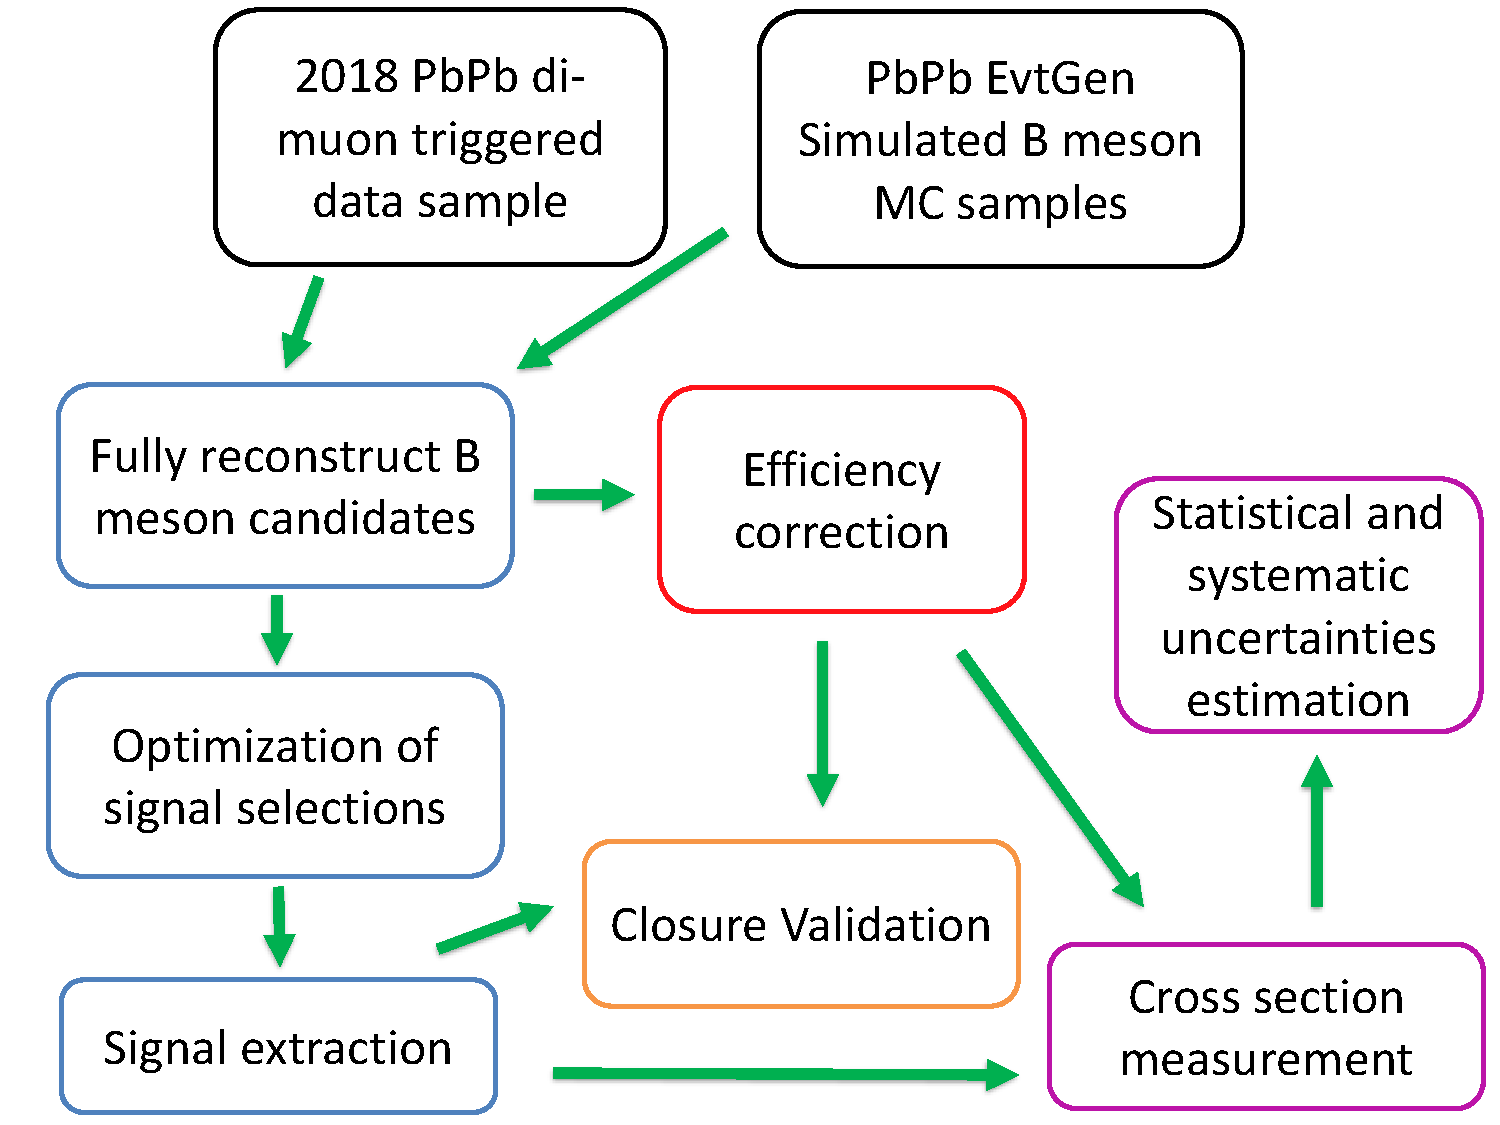
\includegraphics[width=0.75\textwidth]{Figures/Chapter5/BsBPWorkFlow.pdf}
\caption{The block diagram of the workflow with major steps for both B-meson cross section measurements is shown above.}
\label{BsBPWorkFlow}
\end{center}
\end{figure} 

Figure \ref{BsBPRECO} shows pictorially the decay topology of fully reconstructed B meson and our reconstruction strategies

\begin{figure}[hbtp]
\begin{center}
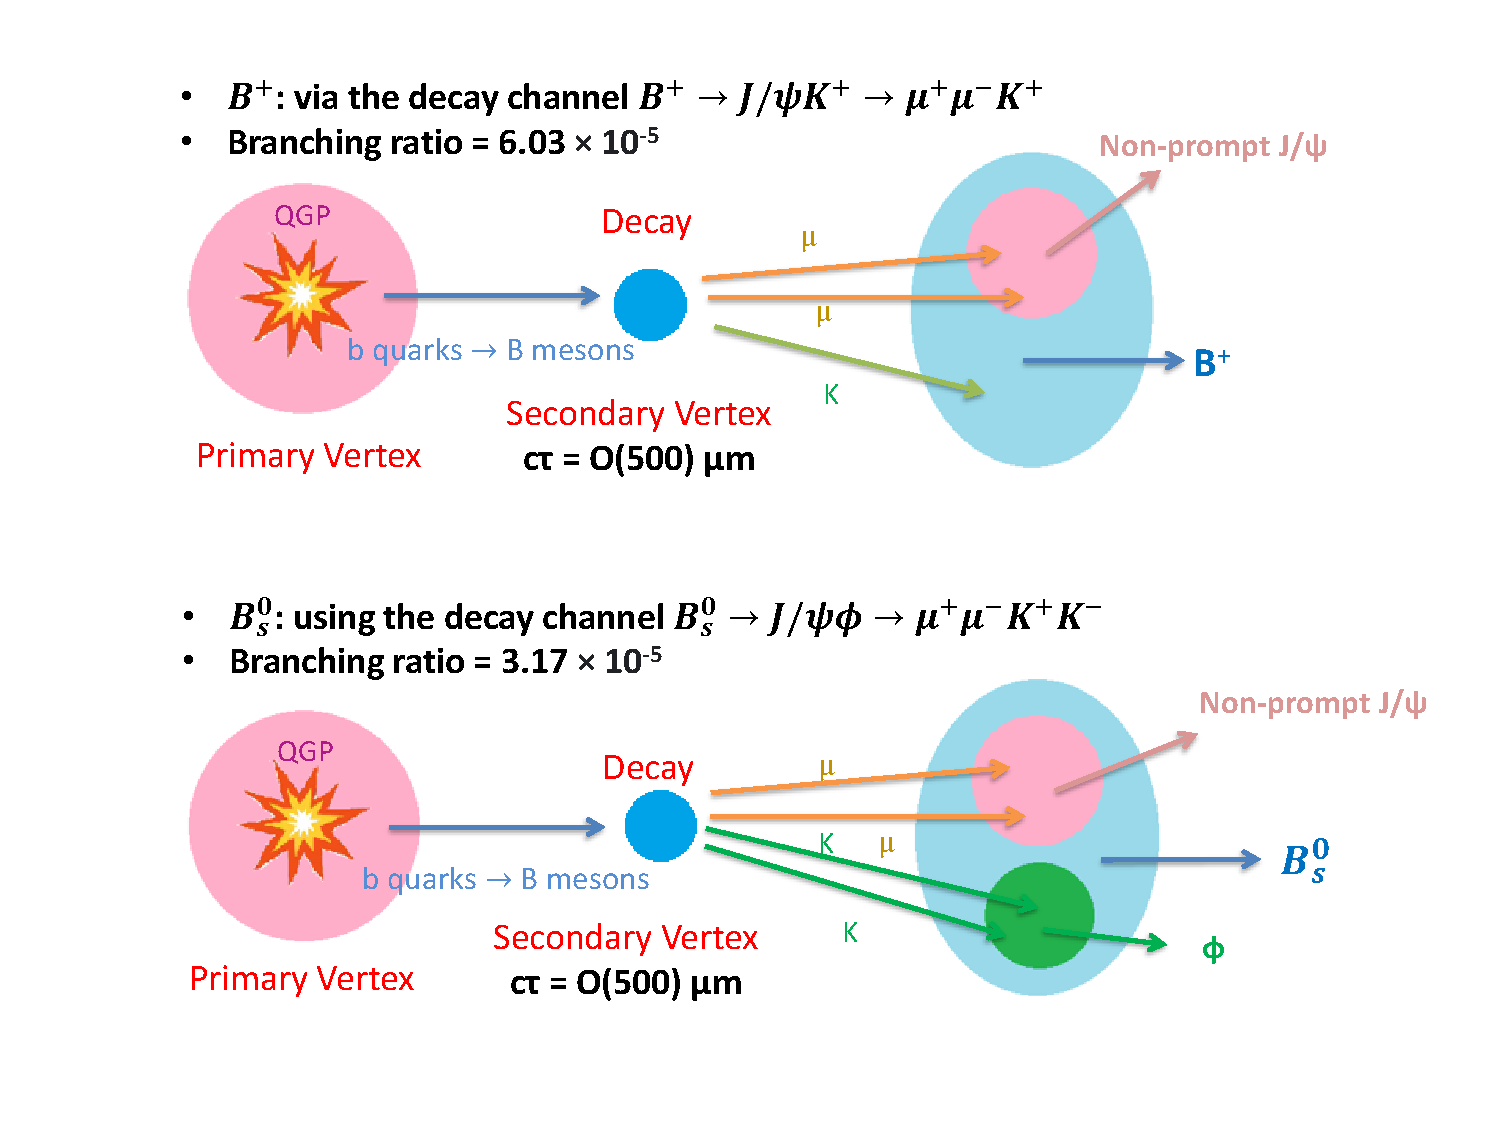
\includegraphics[width=1.05\textwidth]{Figures/Chapter5/BsBPRECO.pdf}
\caption{The strategies to fully reconstruct $B^0_s$ and $B^+$ in the selected exclusive decay modes are shown above.}
\label{BsBPRECO}
\end{center}
\end{figure} 

In this thesis, we propose to measure $B^0_s$ and $B^+$ cross section in the $p_T$ bin of [7, 10, 15, 20, 50] GeV/c within centrality [0, 90] and centrality bin of [0, 30, 90] with $p_T$ [10, 50]. The rapidity range of B-meson measurements is confined in $B |y| < 2.4$.

\subsection{Technical Challenges}

Despite the excellent muon, tracking, vertexing capabilities of the CMS detector, there are still many challenges for the analysis. Below is a list of challenges in the B-meson analysis 

\begin{itemize}
\item The small B-meson decay branching ratio, which on in the order of 10$^{-5}$, and limited luminosity of the sample: $S \downarrow$ 
\item Huge combinatorial background without hadron particle identification, particularly in PbPb collisions and at low $p_T$:  $B \uparrow$ 
\item Low muon acceptance of at very low $p_T$: $S \downarrow$ 
\item High fake track rate with low tracking efficiency at very low $p_T$: $B \uparrow$ 
\end{itemize}

Here, $S$ stands for signal and $B$ stands for background. These factors will all lower the signal-to-background ratio, which makes challenging to fully reconstruct B mesons, particularly at very low $p_T$. In this thesis, to reduce the signal to background ratio and the systematic uncertainties, we will employ a novel machine learning along with a multivariate analysis approach and the elaborated single-particle efficiency correction method to perform the measurements.


\section{Analysis Samples}


\subsection{Dimuon Triggered Datasets}

In this part of the thesis, I focus on studying beauty production and hadronization in QGP. Therefore, this analysis is performed using the 2018 PbPb data at $\sqrt{s_{NN}}$=5.02 TeV, which has an integrated luminosity of 1.7 $nb^{-1}$. 
The analysis uses the dimuon primary datasets (\textit{DoubleMu} PD). The full name of the used datasets and their corresponding luminosity can be found in Table~\ref{tab:lumi}.

\begin{table}[htb]
\begin{center}
\caption{List of PbPb HLT datasets and triggers with the corresponding integrated luminosities used in the analysis.}
\label{tab:lumi}
 \tiny
 \begin{tabular}{ l | l | l | l | }
 System& Primary dataset & Trigger & Luminosity\\
  \hline\hline 
PbPb & \verb#/HIDoubleMuonPsiPeri/HIRun2018A-04Apr2019-v1/AOD# & \verb# HLT_HIL3Mu0NHitQ10_L2Mu0_MAXdR3p5_M1to5_v1 # & 522 $nb^{-1}$\\
  PbPb & \verb#/HIDoubleMuon/HIRun2018A-04Apr2019-v1/AOD # & \verb# HLT_HIL3Mu0NHitQ10_L2Mu0_MAXdR3p5_M1to5_v1 # & 1124 $nb^{-1}$ \\
  \hline
  PbPb & Combined All & & 1.657 ($\sim$ 1.7) $nb^{-1}$ \\
 \end{tabular}
\end{center}
\end{table}

The details of the dimuon trigger selection to collect the data sample are explained in 2.2.5. In addition, a Muon JSON to select good luminosity sections in the PbPb dataset is applied. Both $B^0_s$ and $B^+$ data come from this sample. However, in the later stage, the B-meson candidates are saved in different channels based on the reconstruction.

\subsection{Monte Carlo Simulations Samples}

Dedicated PbPb $B^0_s$ and $B^+$ samples are generated in order to estimate the acceptance and selection efficiencies, to study the background components, and to evaluate systematic uncertainties. {\sc PYTHIA8} Tune CUETPM8~\cite{PYTHIAFrag,PYTHIA2}, set to generate inclusive (all quark/antiquark, as well as gluon initiated) QCD processes, was used to generate at 5.02 TeV the signal. Several preselections at the generation steps are applied in order to optimize the generation process and conserve resources.

For $B^0_s$, only signal events were kept with at least one $B^0_s$ (forced to decay through the channel $B^0_s \rightarrow J/\psi \phi \rightarrow \mu^+\mu^-K^+K^-$ by means of the {\sc evtgen} package~\cite{EvtGen}), with $p_{T}>$ 5.0 GeV/c, and $|\eta|<$ 2.4. In addition, the $J/\psi$ and $\phi$ meson, are forced to decay in the two muons and two kaons respectively. Final state radiations are generated using {\sc photos}~\cite{PHOTOS}. The selected signal B mesons {\sc PYTHIA8} events were embedded into a PbPb background simulated with the {\sc HYDJET}  (version 1.8, tune ``Drum'' for the prompt and non-prompt $J/\psi$ MC and tune "Cymbal5Ev8" for the $B^0_s$ signal MC)~\cite{HYDJET} event generator.

For $B^+$, similar requirements for MC generation are applied except a different decay channel $B^+ \rightarrow J/\psi K^+ \rightarrow \mu^+\mu^-K^+$ is used.

For $B^0_s$ and $B^+$, around fifty thousand events were generated in 5 $\hat{p}_{T}$ bins, with boundaries of $\hat{p}_{T} >$ 0, 5, 15, 30, 50, in both signal only, and embedded samples. The high $\hat{p}_{T}$ selections are used to enrich the high $p_T$ B-meson statistics in order to perform efficiency correction. 

We should note that there are two components in the MC sample. The truth information about the particles generated in the simulation, which is called generated (GEN), and the reconstructed one smeared according to the CMS detector effects, which is called reconstructed (RECO). Due to the nature of MC generation, we will need to reweigh on MC in order to model the data.

In addition to the $B^0_s$ and $B^+$, a sample of inclusive b hadron to $J/\psi$ (non-prompt) MC is also simulated to study the possible background contribution to the B-meson analysis due to 


\subsection{$\hat{p}_{T}$ Reweighing}


As mentioned above, different $\hat{p}_{T}$ cuts are applied to generate the MC samples. When merging the samplings, a  $\hat{p}_{T}$ weight based on beauty production cross section is required to apply to the MC in order to obtain a smooth distribution that can model the real data. Figure \ref{GENPTDIS} shows the generated $p_T$ ($Gp_T$) distribution of $J/\psi$, $B^+$ , and $B^0_s$ before and after applying the $\hat{p}_{T}$ weight:


\begin{figure}[h]
\begin{center}
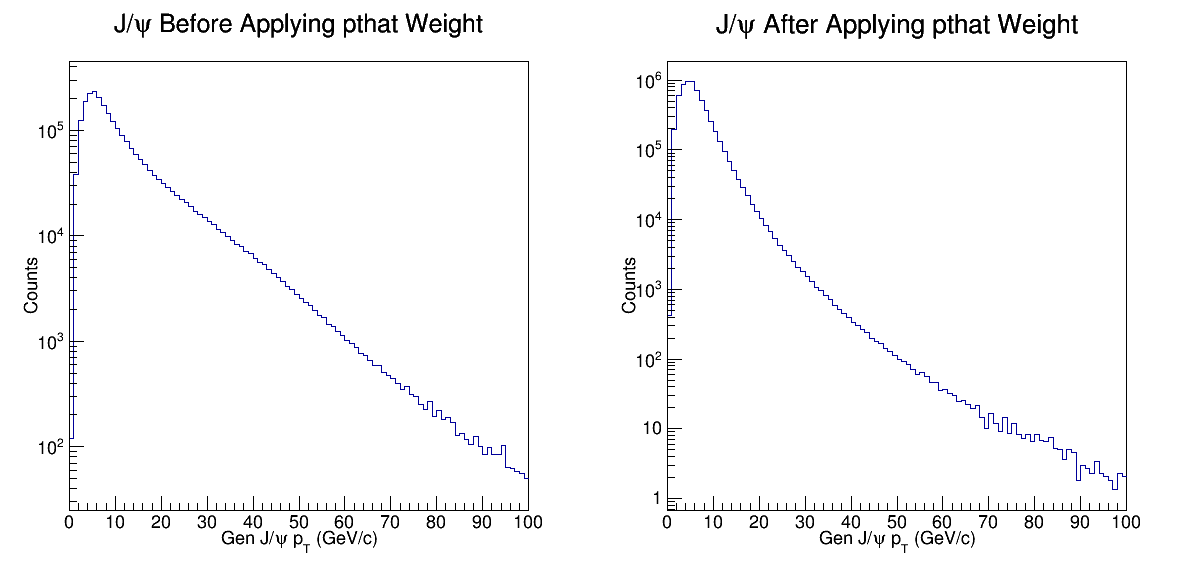
\includegraphics[width= 0.90\textwidth]{Figures/Chapter5/JPsiGenpT.png}
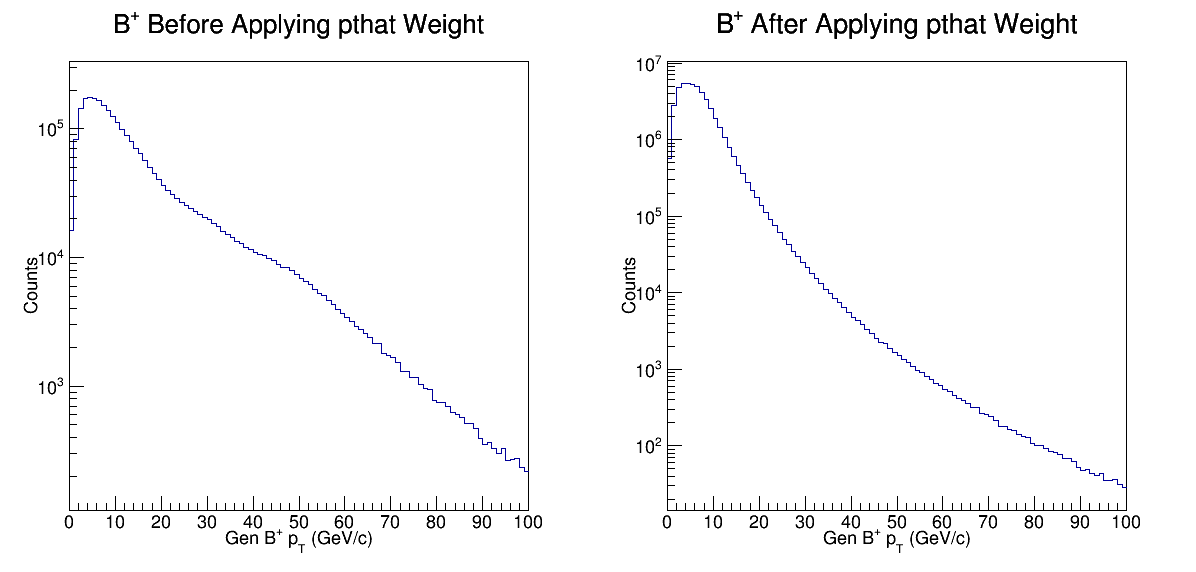
\includegraphics[width= 0.90\textwidth]{Figures/Chapter5/BPlusGenpT.png}
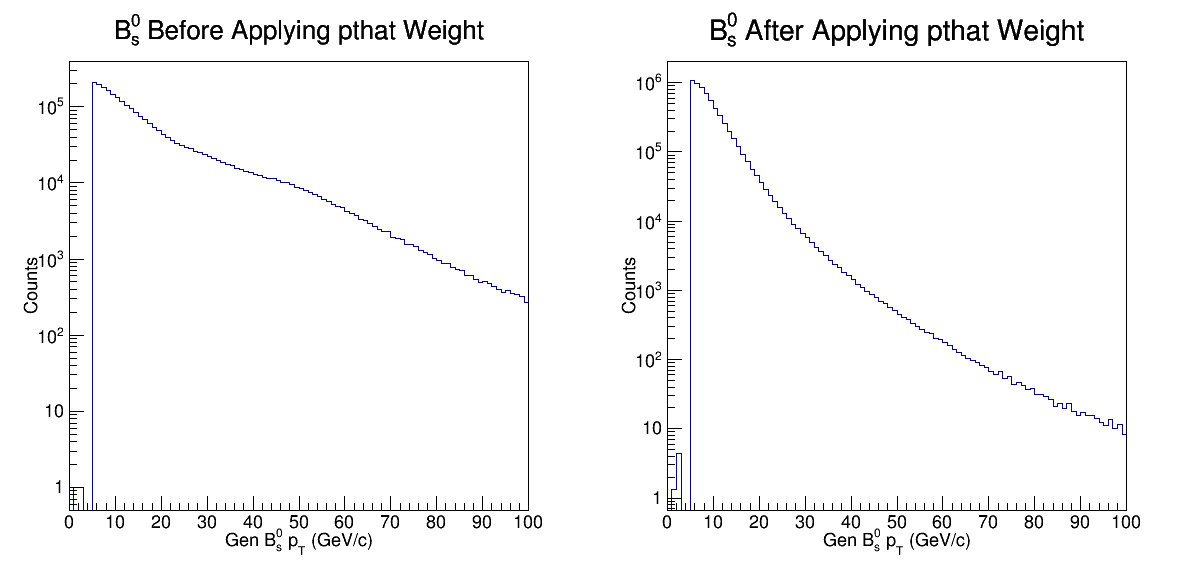
\includegraphics[width= 0.90\textwidth]{Figures/Chapter5/BsGenpT.png}
\caption{ $J/\psi$ generated $p_{T}$ distribution before (upper left) and after (upper right) $\hat p_{T}$ reweighing, $B^+$ generated $p_{T}$ distribution before (middle left) and after (middle right) $\hat p_{T}$ reweighing, and $B_s^0$ generated $Gp_{T}$ distribution before (lower left) and after (lower right) $\hat p_{T}$ reweighing are shown above.}
\label{GENPTDIS}
\end{center}
\end{figure}


\subsection{RECO B-meson ${p}_{T}$ Reweighing}

Then, we also check if this smooth $Gp_T$ shape in fact correspond to a good agreement between the data and MC in the RECO side. Therefore, we take the ratio of the normalized data raw yield to the normalized MC raw yield and perform a variety of functions to fit the distribution. In our studies, we use Linear ($y = p_0 + p_1 x$), Quadratic ($y = p_0 + p_1 x + p_2 x^2$), Linear + Inverse  ($y = p_1 x + \frac{p_2}{x}$), Linear + Square Root ($y = p_0 + p_1 x + p_2 \sqrt{x}$), Linear + Log ($y = p_0 + p_1 x + p_2 \log{x}$). The data vs MC raw yield shape and our fitting results on spectra ratio are show as follows \ref{BsBptWeight} and  \ref{BPBptWeight} for $B^0_s$ and $B^+$ respectfully 



\begin{figure}[h]
\begin{center}
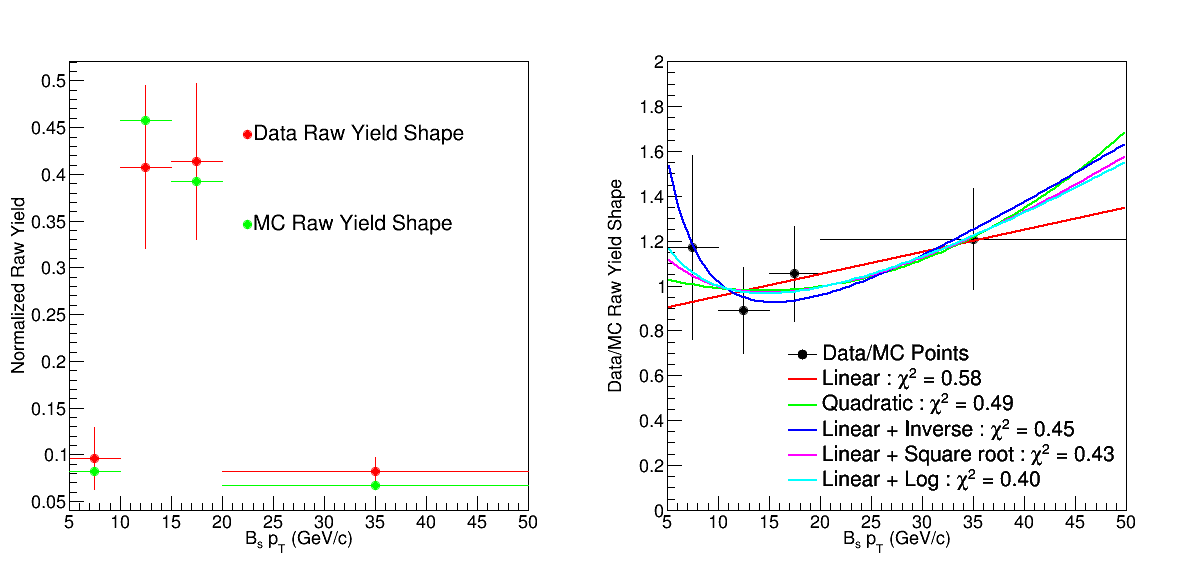
\includegraphics[width= 0.97\textwidth]{Figures/Chapter5/BsBptDataMC.png}
%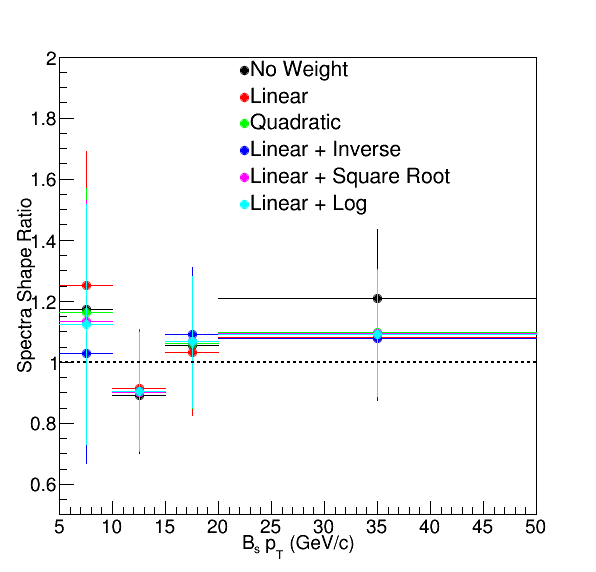
\includegraphics[width= 0.55\textwidth]{Figures/Chapter5/BsBptDataMCAfter.png}
%\caption{ $B^0_s$ $p_T$ normalized raw yields obtained in PbPb MC and Data are shown above on the top left panel. The data/MC ratio and different fitting functions: Linear (Red), Quadratic(Green), Linear + Inverse (Blue), Linear + Square Root (Purple), and Linear + Log (Cyan) and their $\chi^2$ are shown above on the top right panel. The bottom plots are the data/MC reweighed yields with different functions from the fit on the top right panel. We can see that they all get closer to unity compared unweighted MC. The Linear + Log (Cyan) line, which has the smallest $\chi^2$ and is closest to unity after applying the weight to the MC. Hence, Linear + Log function is use as nominal for our $B^0_s$ $p_{T}$ reweighing. All other fitting function are used as reference to calculate the $p_T$ shape systematic uncertainties.}
\caption{ $B^0_s$ $p_T$ normalized raw yields obtained in PbPb MC and Data are shown above on the top left panel. The data/MC ratio and different fitting functions: Linear (Red), Quadratic(Green), Linear + Inverse (Blue), Linear + Square Root (Purple), and Linear + Log (Cyan) and their $\chi^2$ are shown above on the top right panel. The bottom plots are the data/MC reweighed yields with different functions from the fit on the top right panel.}
\label{BsBptWeight}
\end{center}
\end{figure}

\begin{figure}[h]
\begin{center}
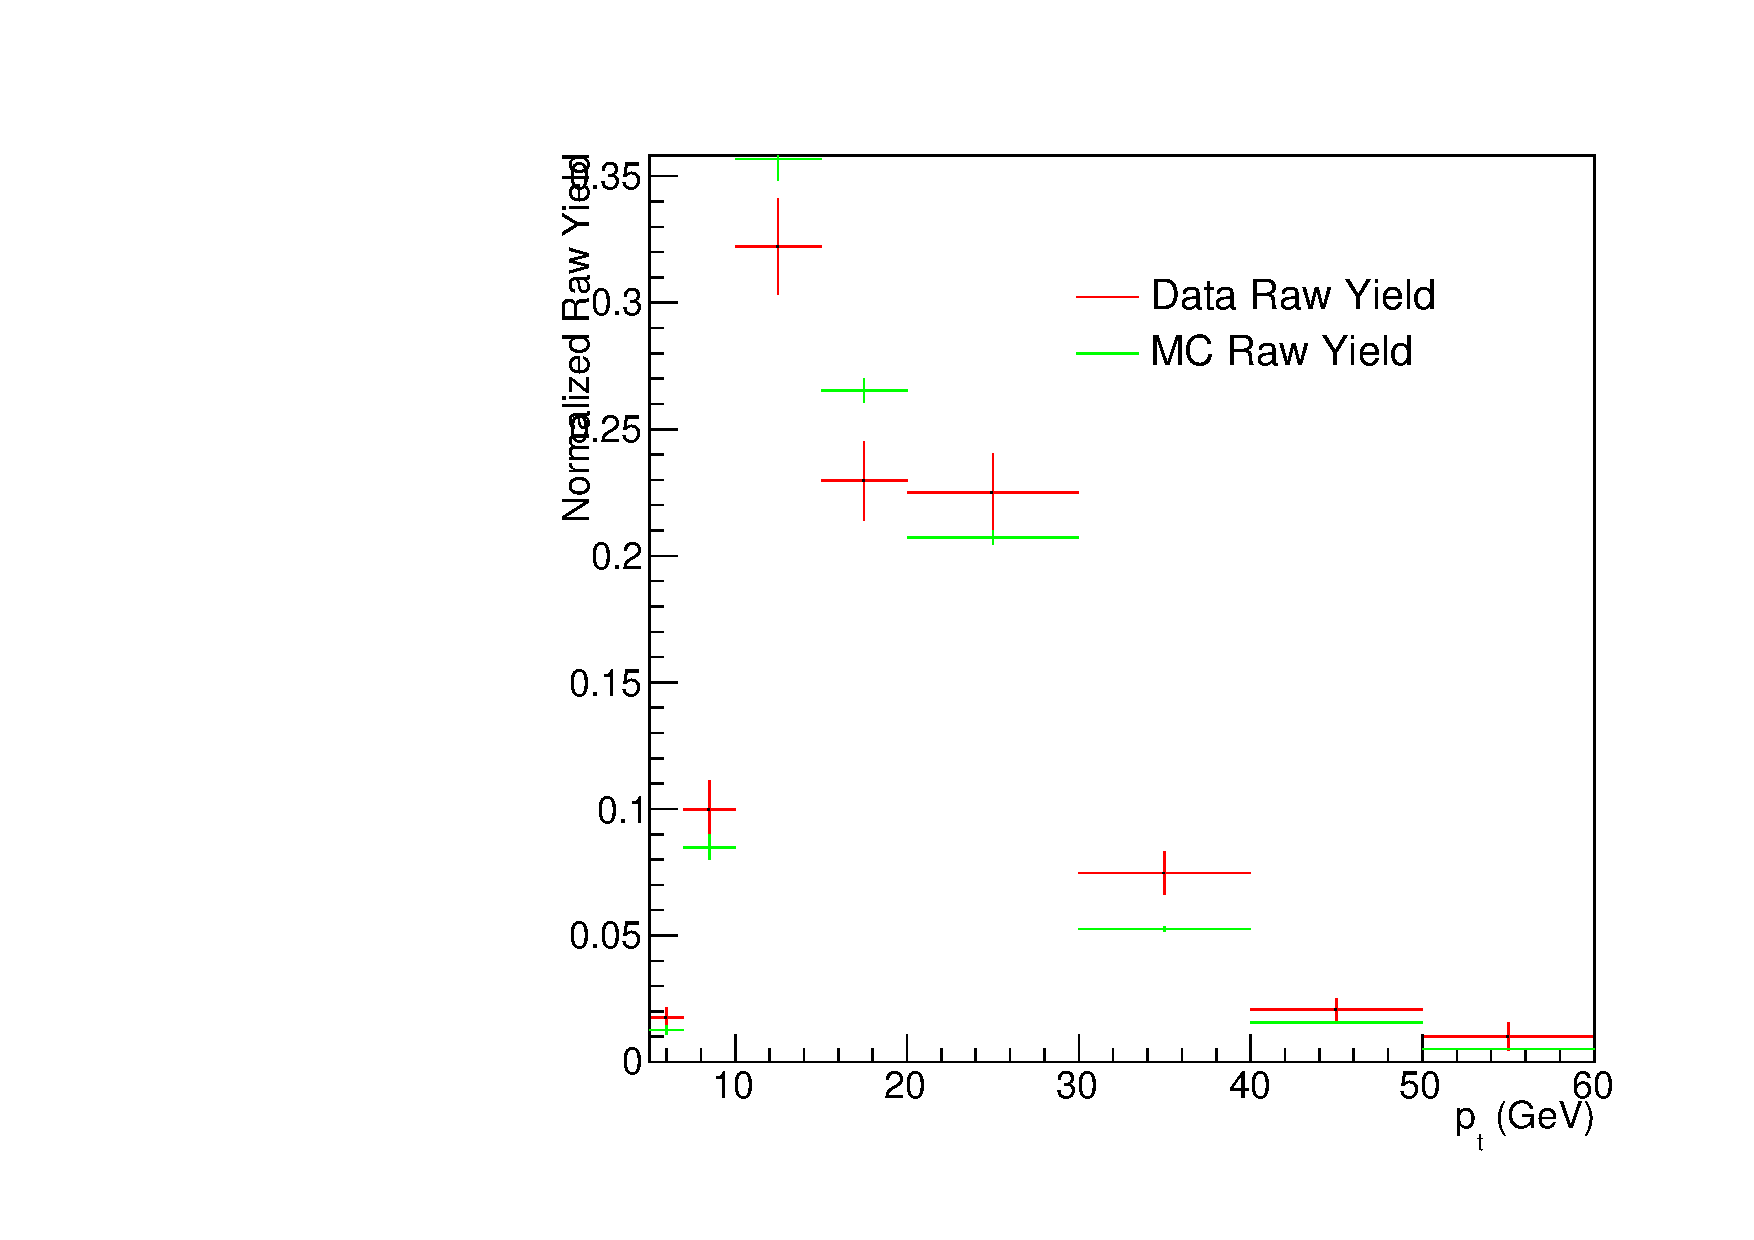
\includegraphics[width= 0.48\textwidth]{Figures/Chapter5/BPBptDataMC1.pdf}
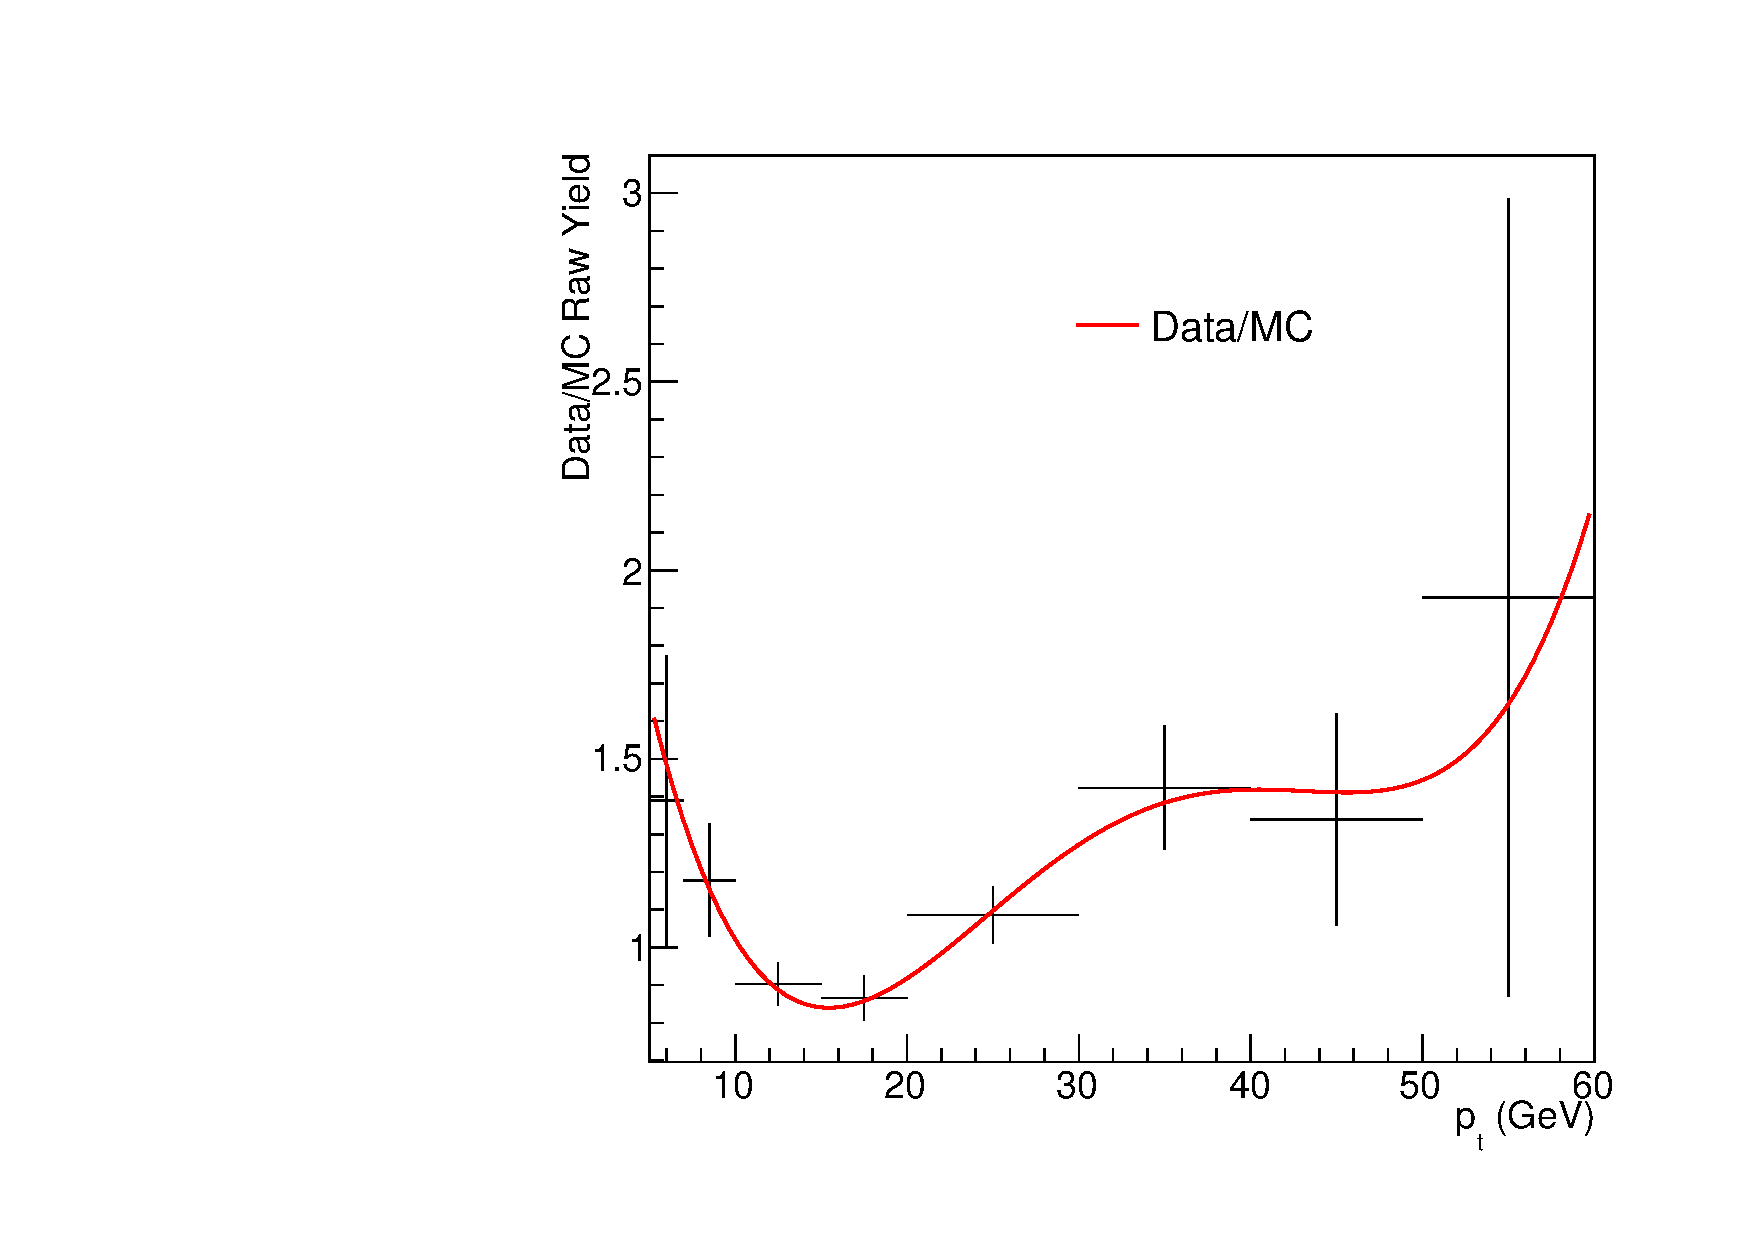
\includegraphics[width= 0.48\textwidth]{Figures/Chapter5/BPBptDataMC2.pdf}
\caption{The normalized $B^+$ raw yield in MC (green) and Data (red) as a function RECO $B^+$ $p_T$ (left) and the fourth-order polynomial fits to their ratio (right) are shown above.}
\label{BPBptWeight}
\end{center}
\end{figure}


\subsection{Centrality Reweighing}

Because the MC simulations employ PYTHIA embedded into a PbPb background simulated, they do not model the centrality of nucleus-nucleus collision well. Therefore, the MC simulations are also reweighed in order to match the centrality distribution in data. In the middle panel of Figure \ref{CentComp}, the centrality distribution of the MC simulation (red) is compared to the one in data (blue), before the re-weighting. Each unit (hiBin) on the x-axis represents 0.5\% centrality. The number of binary collisions $N_{coll}$ was used as the weight to scale the MC centrality, and the distribution presented in the right panel of Figure 4 was obtained. 

\begin{figure}[hbtp]
\begin{center}
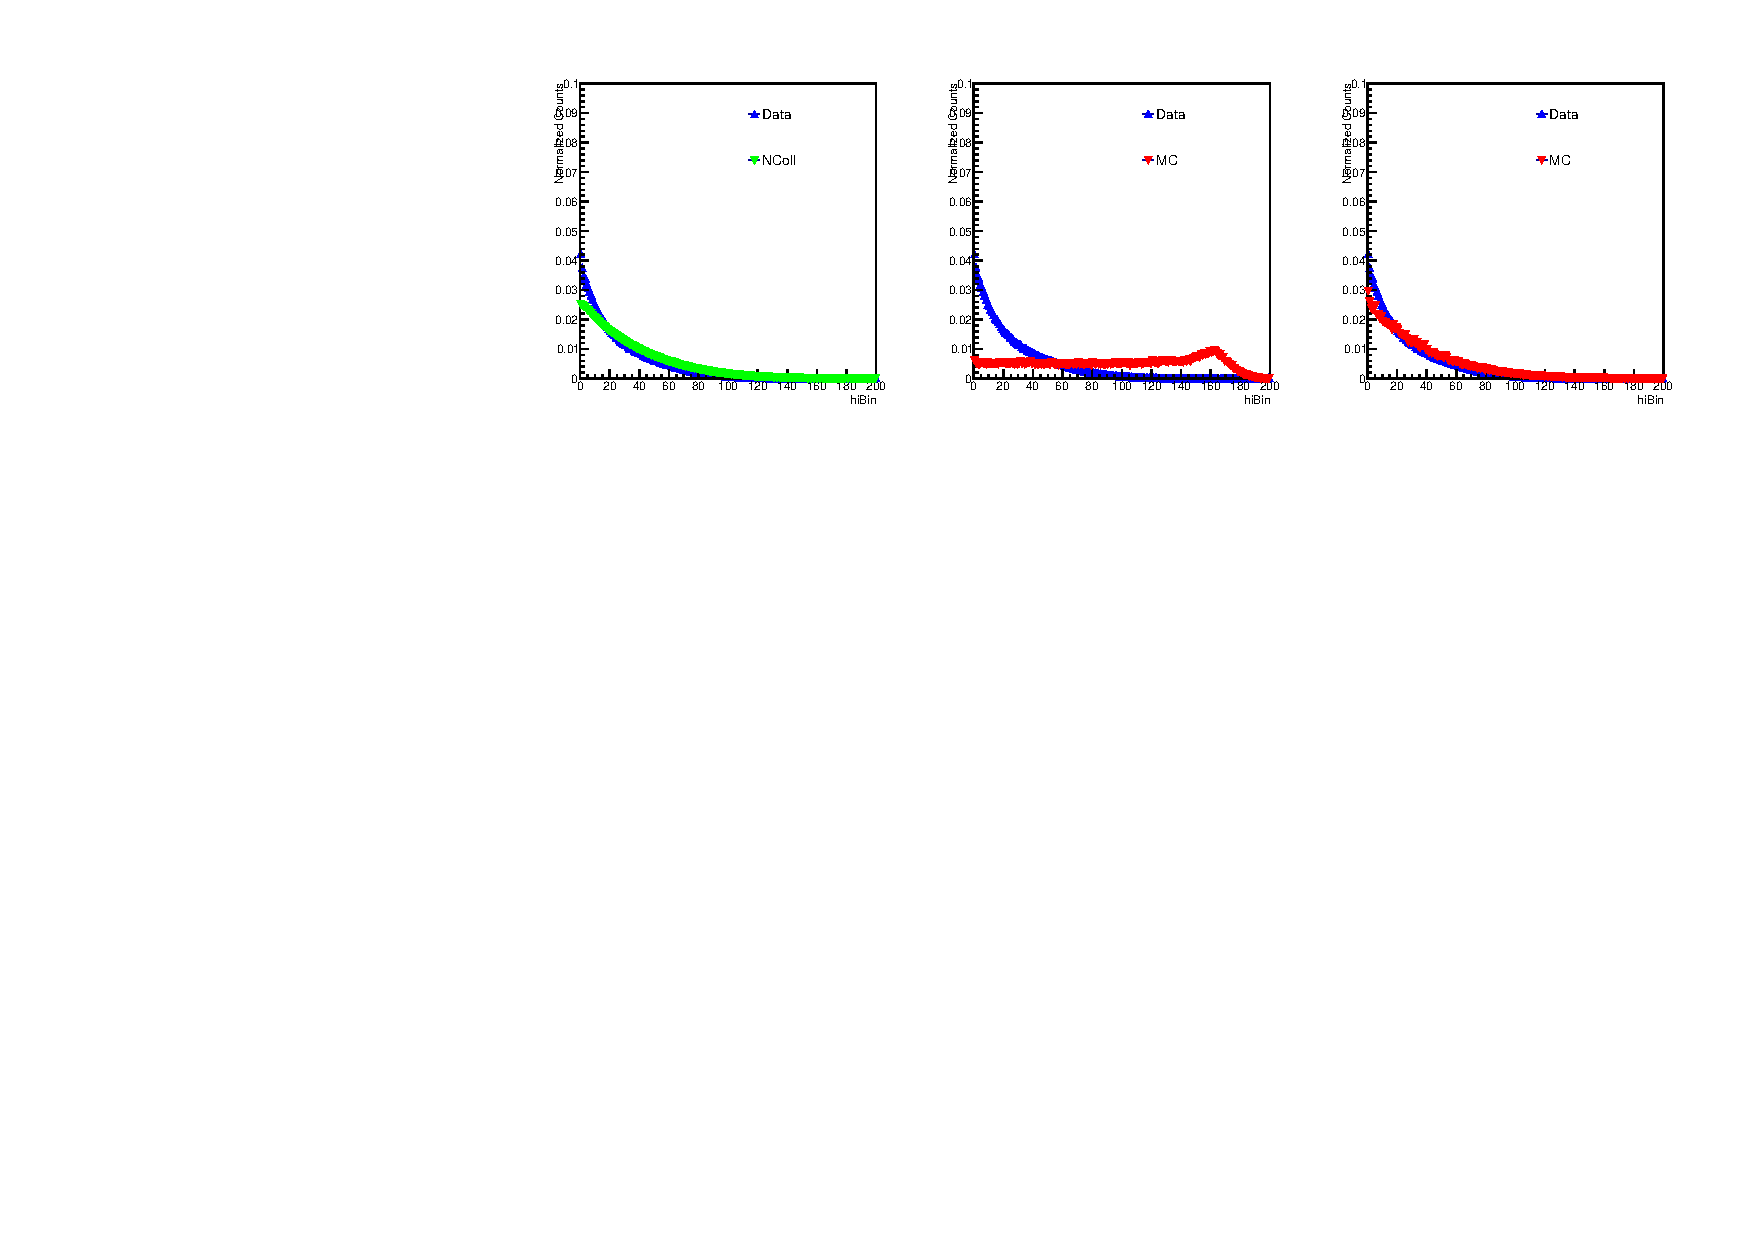
\includegraphics[width=1.10\textwidth]{Figures/Chapter5/CentralityWeight.pdf}
\caption{The comparison between $N_{coll}$ and Data vs hiBin (left), centrality distribution of MC (red) and data (blue) in PbPb collisions in the centrality interval 0-100\% without $N_{coll}$ weight (middle), and with $N_{coll}$ weight (right) are shown above.}
\label{CentComp}
\end{center}
\end{figure} 


A better centrality agreement between the data and the MC is seen after the reweighing process. 

\subsection{PV$_{z}$ Reweighing}


In addition to $p_T$ shape and centrality reweighing, there must be a primary vertex $z$ position (PV$_{z}$) reweighing due to incorrect modeling of the primary vertex location and resolution in the MC simulation. In fact, it is known that the MB samples used to embed for PbPb signal MC samples (with Cymbal5Ev8 tune) have PV$_{z}$ offsets. Also, the offsets between data and MC in the X and Y directions are observed in the 2018 PbPb collisions. To remedy this, a Gaussian fit is applied to both the data and MC PV$_{z}$ distributions, as showed in Fig.~\ref{PVZPlot}. The black markers represent the distribution points for MC (left), and data (right), while the red line represents the fit result. Then, the ratio between the two fit results is taken as the weighting function. The result after this weighting can be found in Fig. \ref{PVZPlot} But we should note that this analysis is not sensitive to the absolute value of the PV position because the reconstruction of the B-meson relies only on the relative distance between PV and B-meson reconstructed vertex which will be presented in the later sections.

\begin{figure}
\begin{center}
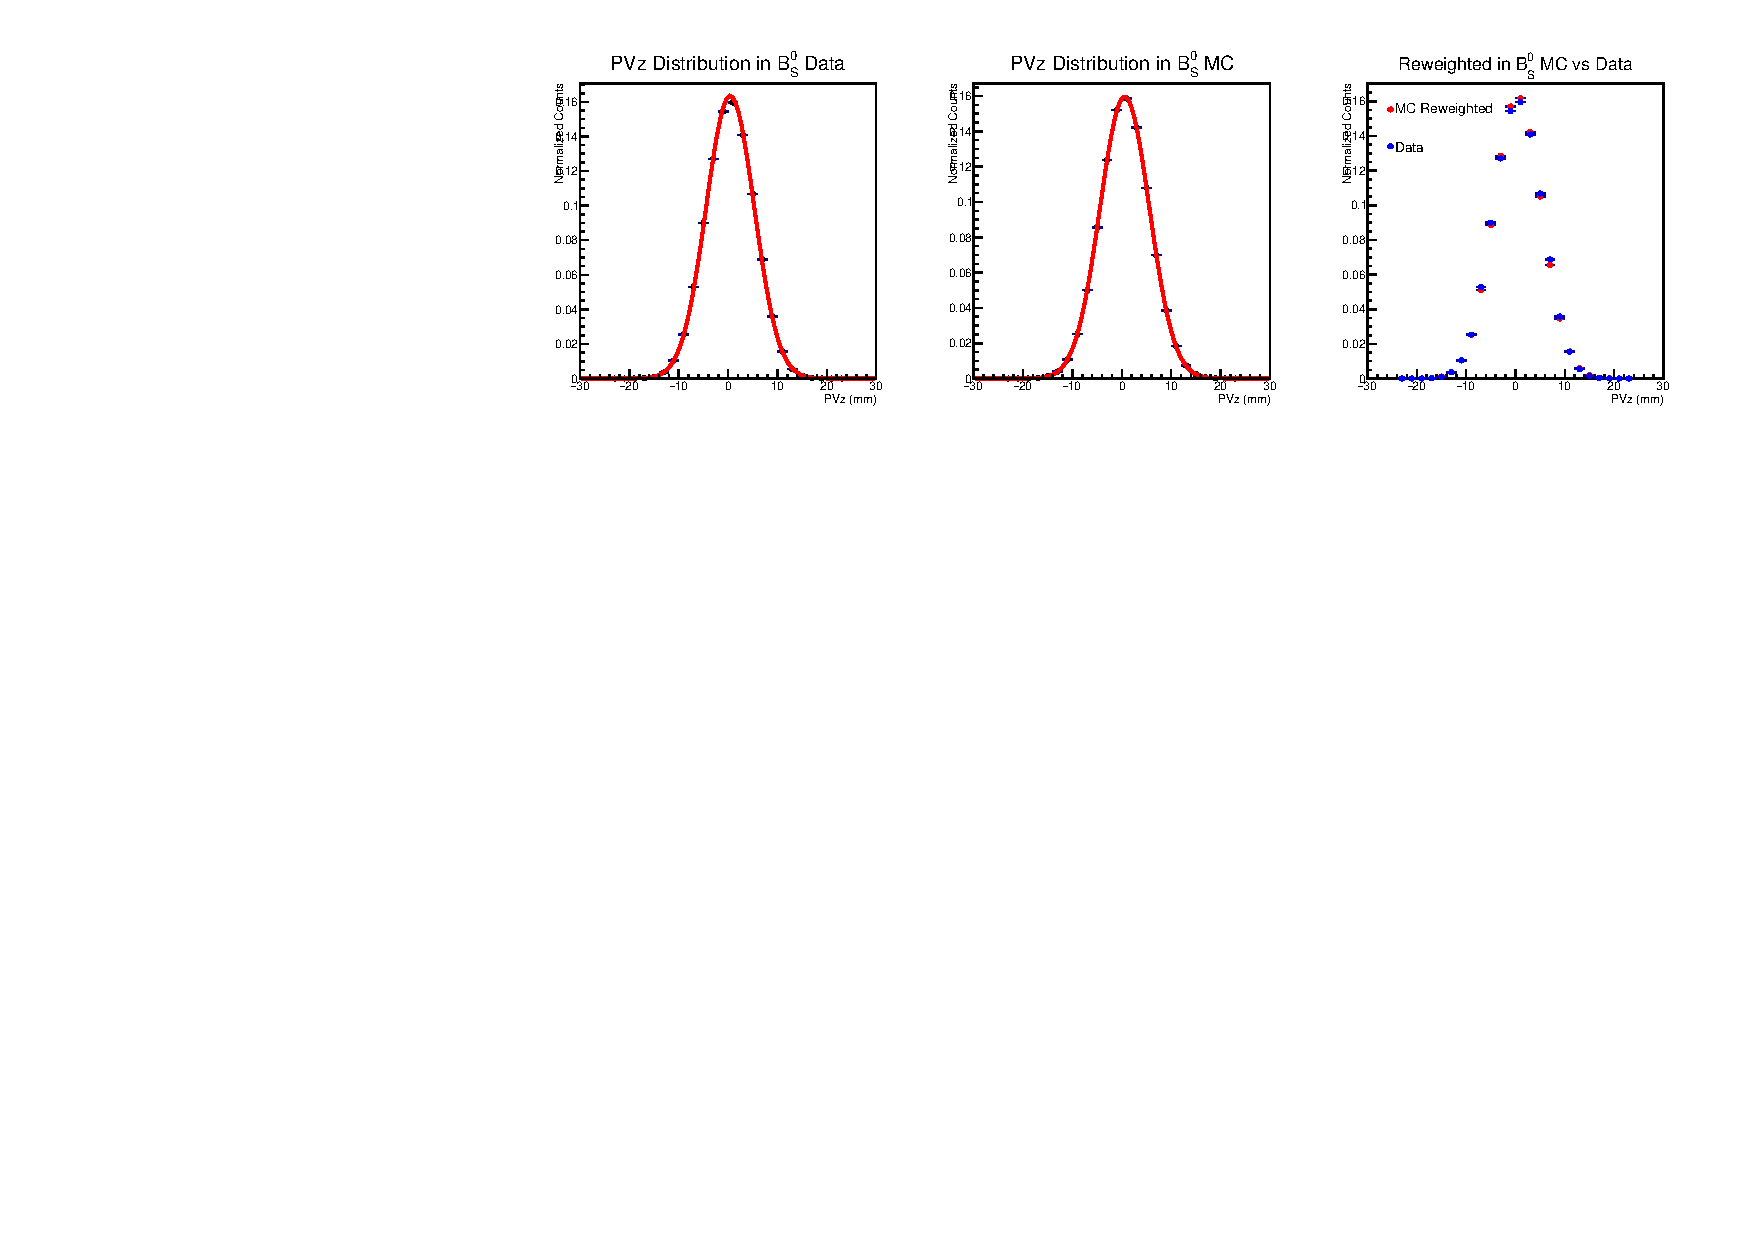
\includegraphics[width= 1.10\textwidth]{Figures/Chapter5/PVzWeightPbPb.pdf}
\caption{PV$_{z}$ distribution, fitted with a gaussian function in PbPb MC simulations (left), in PbPb data (middle), PV$_{z}$ reweighed MC to data with the ratio of data-to-MC Gaussian Fits (right) are shown above. The PV$_z$ distributions are well described by the Gaussian function and reweighing reduces the MC-data discrepancy.}
\label{PVZPlot}
\end{center}
\end{figure}

An almost perfect MC-data agreement after PV$_{z}$ reweighed is observed above. After these standard reweighing procedures, the residue disagreement between MC and data will be considered as a source of systematic uncertainties.


\clearpage

\section{Global Event Observables} 

The global event observables characterize general conditions of heavy-ion collision. In this analysis, we decide to use another set of quantities including the total number of MB events to represent the luminosity and the average number of participants $\langle N_{parts} \rangle$ to represent centrality. In addition, to compare with $pp$ collisions, we also need to scale the cross section in PbPb according to $N_{coll}$. Therefore, we will determine all the global event observables including the total number of minimum bias events ($N_{MB}$), centrality, number of participant nucleons $N_{part}$, number of binary collisions $N_{coll}$, and nuclear overlapping function $T_{AA}$ in dimuon PbPb dataset in the following subsections.

\subsection{Total Number of Events}

As seen in Table \ref{tab:lumi}, the nominal luminosity of the dimuon PbPb dataset 1.7 $nb^{-1}$. However, this nominal luminosity has large uncertainties and should be used in the analysis to measure the cross section. As mentioned previously in Chapter 2.2, the dimuon trigger, based on the MB trigger, will not save events that do not pass trigger selections. Hence, we can use the events of 1 PD MB datasets (PD0) via the following formula to determine the actual number of MB events corresponding to the dimuon PbPb datasets: 


\begin{equation}
N_{MB} = \frac{N^{\mu\mu json}_{MB}}{\mathcal{L}_{MB trigger}^{\mu json}} \mathcal{L}_{\mu\mu trigger}^{\mu\mu json}
\end{equation}

The definition of the variables in the formula are as follows:


\textbf{$N_{MB}$:} The number of minimum bias events in dimuon PD with Muon JSON.

\textbf{$N^{\mu json}_{MB}$:} The number of the event of all MB PDs with Muon JSON. 

\textbf{$\mathcal{L}^{\mu json}_{MB}$:} The luminosity of all MB PDs with Muon JSON.

\textbf{$\mathcal{L}_{\mu\mu trigger}^{\mu\mu json}$:} The luminosity of dimuon PD with Muon JSON.

\iffalse 

To obtain the total number of minimum bias $N_{MB}$, first we process one PD (PD5) minimum bias events and count the total number of events for centrality at 0 - 90\% to obtain $N^{\mu\mu json}_{MB}$. Then, we run the brilcal for MB PD5 and sum the luminosity of HLT MB triggers: 

Trigger 1: ``HLT\_HIMinimumBias\_part0\_v1" 
 
Trigger 2: ``HLT\_HIMinimumBias\_SinglePixelTrack\_part0\_v1"
 
Trigger 3: ``HLT\_HIMinimumBias\_SinglePixelTrack\_NpixBypass\_part0\_v1" 
  
Trigger 4: ``HLT\_HIMinimumBias\_SinglePixelTrack\_NpixGated\_part0\_v1" 
 
to obtain $\mathcal{L}^{\mu\mu json}_{MB}$. 

Trigger 5: ``HLT\_HIL3Mu0NHitQ10\_L2Mu0\_MAXdR3p5\_M1to5\_v1" 

to obtain $\mathcal{L}^{\mu\mu json}_{MB}$. 

Table ~\ref{tab:lumibreadown} shows the luminosity of Trigger 1 -- 5 above. The sum of trigger 1 -- 4 will be $\mathcal{L}^{\mu\mu json}_{MB}$ and trigger 5 will be $\mathcal{L}^{\mu\mu json}_{MB}$.

\begin{table}[h]
\begin{center}
\caption{Summary table of the luminosity of HLT triggers to obtain the number of minimum biased events.}
\vspace{1em}
\label{tab:lumibreadown}
  \begin{tabular}{ |c | c| }
      \hline
   HLT  & Luminosity ($\mu b^{-1}$)  \\
    \hline
    \hline 
 HLT\_HIMinimumBias\_part0\_v1        & 14.8269  \\
 `HLT\_HIMinimumBias\_SinglePixelTrack\_part0\_v1  & 1.3010  \\
HLT\_HIMinimumBias\_SinglePixelTrack\_NpixBypass\_part0\_v1 & 7.9468 \\
HLT\_HIMinimumBias\_SinglePixelTrack\_NpixGated\_part0\_v1 &  \\
    \hline 
Total & 24.0748  \\
    \hline 
HLT\_HIL3Mu0NHitQ10\_L2Mu0\_MAXdR3p5\_M1to5\_v1  & 1657.1320 \\
     \hline
    \hline
\end{tabular}
\end{center}
\end{table}


We have also obtained the number of events by processing one of the MB sample. The total number of events can be found in Table \ref{tab:NMBEventsCent}. 

\begin{table}[h]
\begin{center}
\caption{Summary table of the total number of MB events vs centrality}
\vspace{1em}
\label{tab:NMBEventsCent}
  \begin{tabular}{ |c | c| }
    \hline 
Centrality & $ \mathcal{L}_{\mu\mu trigger}^{\mu\mu json}$ \\
     \hline
         \hline
0-10\% & 18276069  \\
10-20\%& 17680482  \\
20-30\% & 17687566 \\
30-40\% & 17684913 \\
40-50\% & 17685909 \\
50-60\% & 17680807 \\
60-70\% & 17686640 \\
70-80\% & 18375623 \\
80-90\% & 18749965 \\
0-30\% & 53644117 \\
30-90\% & 107863857 \\
0-90\% & 161507974 \\
     \hline
    \hline
\end{tabular}
\end{center}
\end{table}

\fi

For 0 - 90\%, $N_{MB}^{\mu json}$ is 161507974. The number of events can then be computed as follows:

\begin{equation}
N_{MB} = \frac{N^{\mu json}_{MB}}{\mathcal{L}_{MB trigger}^{\mu json}} \mathcal{L}_{\mu\mu trigger}^{\mu json} = \frac{1657.1320 \mu b^{-1}}{24.0748  \mu b^{-1}} \times 161507974 =  1.1823737719 \times 10^{10} \simeq  \textbf{11.82 billion}
\end{equation}

Hence, the number of MB events for the dimuon PbPb data is $N_{MB} = $11.82 billion. Below, in Table \ref{NMBUsedCent}, we compile the number of minimum biased events $N_{MB}$ in 0 - 30\%, 30\% - 90\%, and 0 -90\%. 

\begin{table}[h]
\begin{center}
\caption{Summary table of the total number of MB events and their uncertainties vs centrality}
\vspace{1em}
\label{NMBUsedCent}
  \begin{tabular}{ |c | c| c| }
    \hline 
Centrality & $N_{MB}$ (billion) & Uncertainties  \\
     \hline
         \hline
0-30\% &  3.941 & 1.26\% \\
30-90\% & 7.882 & 1.26\% \\
0-90\% & 11.82 & 1.26\% \\
     \hline
    \hline
\end{tabular}
\end{center}
\end{table}

%According to the official results from the CMS Global Observable Group, the number of events we obtains is about $N_{events} =$ 11968044281 $\simeq$ 12.0 billion for (0 - 90\%) centrality from using the brilcal to evaluate the luminosity and process MB PD0--5 with our muon JSON, which is very close our calculations: $N_{events} =$ 11.82 billion. Here, we will use the official results

\subsection{Centrality Definition}

For the 2018 PbPb dataset, the centrality is given in hiBin with a 0.5\% increment. The hiBin is defined based on the HF response (hiHF). According to the Global observable, \ref{hiHFvsCent} is the hiHF as a function of centrality with uncertainties.


\begin{figure}[h]
\begin{center}
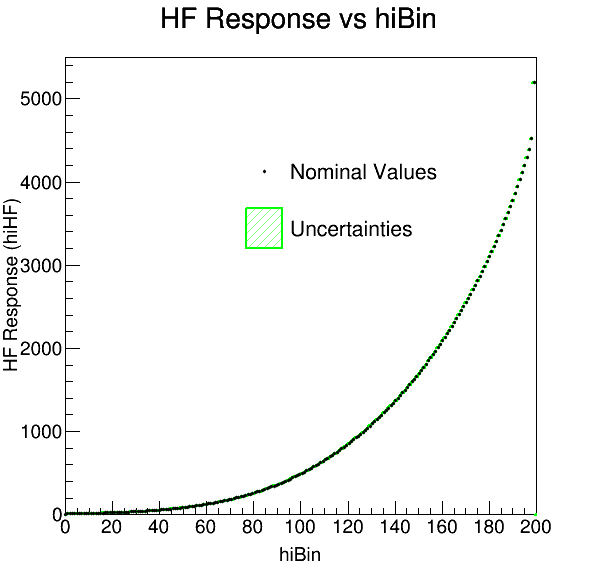
\includegraphics[width= 0.48\textwidth]{Figures/Chapter5/hiHFvsCent.png}
\caption{The nominal (black) and uncertainties band (green) hiHF vs hiBin for CMS 2018 PbPb dataset are shown above.}
\label{hiHFvsCent}
\end{center}
\end{figure}


We can compute the percent deviation nom of final results to estimate systematics due to uncertainties of centrality. 


\subsection{$\langle N_{part} \rangle$, $\langle N_{coll} \rangle$, $\langle T_{AA} \rangle$ vs Centrality}

As we discussed in the Glauber Model \cite{CentPlot,Glauber} section 1.5.7, the number of participant nucleons $N_{part}$, the number of binary nucleon-nucleon collisions, and nuclear overlap function $T_{AA}$ are all functions of the event centrality. The CMS Global Observable group has computed the average $N_{part} $, $N_{coll} $, $T_{AA}$, and their uncertainties  for different centrality bins based on the Glauber Model. The selected results are shown in Table \ref{GOvsCent} below


\begin{table}[h]
\begin{center}
\caption{A summary table of the total number of MB events vs centrality is shown below. The uncertainties are represented in terms of percentage in the parenthesis.}
\vspace{1em}
\label{GOvsCent}
  \begin{tabular}{ |c | c| c| c|}
    \hline 
Centrality &  $\langle N_{part} \rangle$ &$\langle N_{coll} \rangle$  & $\langle T_{AA} \rangle$  \\
     \hline
         \hline
0-30\% &  269.1 (0.39\%)  &  1042 (2.0\%) &	15.42 (2.0\%)   \\
30-90\% & 54.45 (1.5\%)   & 115.2 (3.6\%)  &   1.704 (3.6\%)  \\
0-90\% & 126.0 (0.67\%)   &  424.1(2.2\%)  &    6.274 (2.2\%)  \\
     \hline
    \hline
\end{tabular}
\end{center}
\end{table}

The global observables $N_{MB}$, $N_{part}$, $N_{coll}$, and $T_{AA}$ will be used as input for our B-meson analysis. 

\iffalse

\subsection{Number of Participant Nucleons}

\subsection{Number of Binary Collisions}


\fi

\subsection{Event Multiplicity}

Aside from $N_{MB}$, $N_{part}$, $N_{coll}$, and $T_{AA}$, event multiplicity is also an event observable. We count the number of tracks in each event with some track quality selections and use it to interpret the event multiplicity, which characterizes the event activity. The following is the selection criteria for 

Nevertheless, the event multiplicity is not used in PbPb analysis. It will be used in $pp$ analysis to study the $B^0_s/B^+$ ratio as a function of event multiplicity in $pp$ collisions.

%\section{Monte Carlo Simulations} 

%The Monte Carlo (MC) simulation on the B meson decay is essential to the analysis. It will plays an important role in both the signal extraction and efficiency correction.

%\subsection{PYTHIA}

%\subsection{Hydjet Embedding}

%\subsection{EvtGen Package}

%\subsection{MC reweighing}

\section{B-meson Reconstruction} 

Now we look into each event of the PbPb dimuon dataset. It turns out that there is no PU in any event. Therefore, only one primary vertex for each event. We can then reconstruct the B-meson candidates according to the final state muons and kaons tracks. In CMS, a dedicated software named ``\textit{Bfinder}'' is developed to perform B-meson reconstruction. Figure \ref{BsRECOWF} and Figure \ref{BPRECOWF} show the workflow to fully reconstruct \textit{Bfinder} for $B^0_s$ and $B^+$ respectfully.


\begin{figure}[h]
\begin{center}
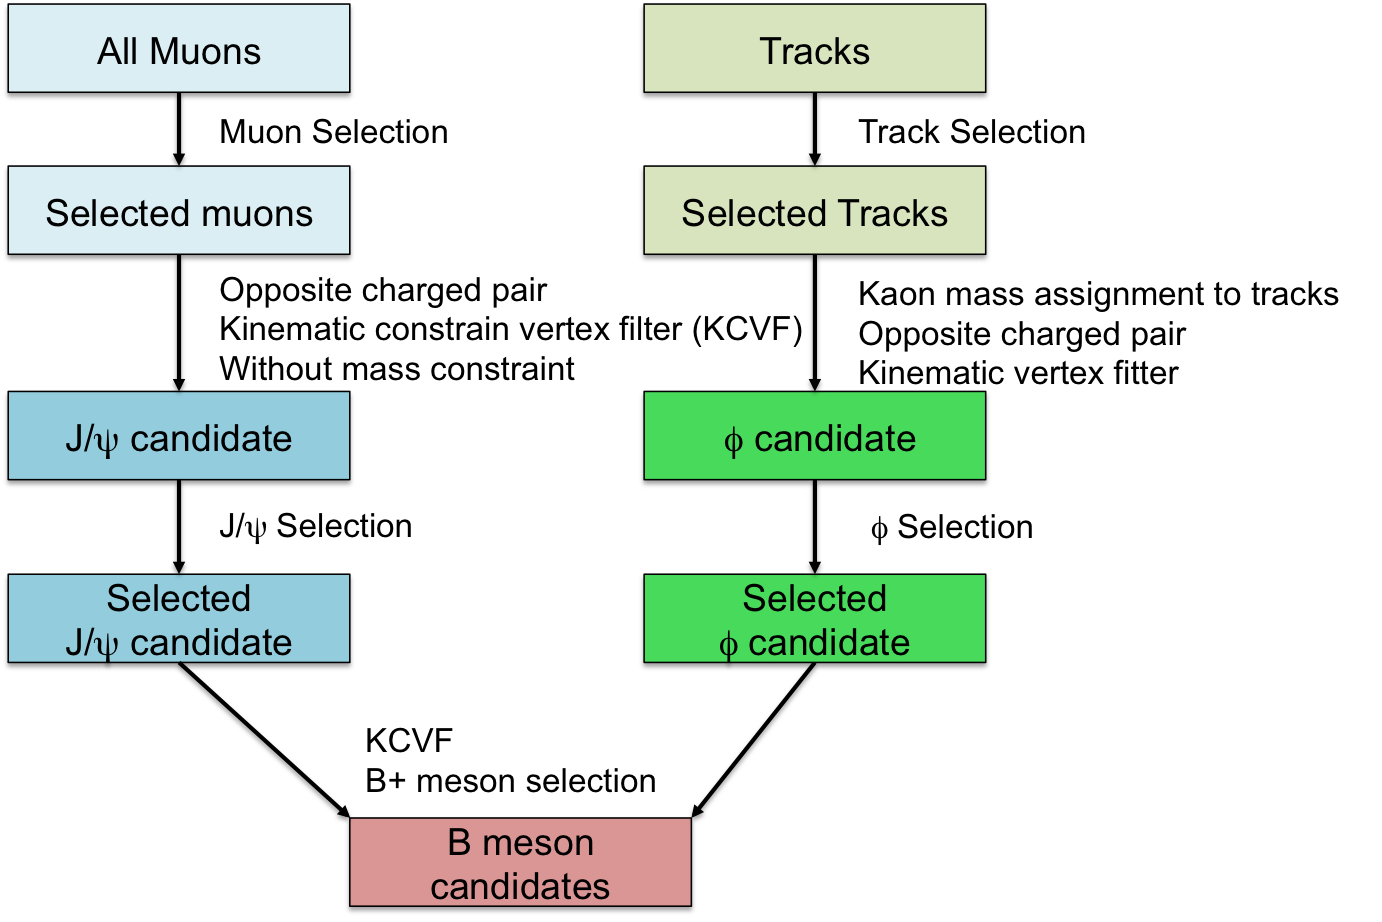
\includegraphics[width= 0.98\textwidth]{Figures/Chapter5/BsmesonWorkflow.png}
\caption{The schematic block diagram of the full reconstruction workflows for $B^0_s$ via the decay channel of $B_s^0 \rightarrow J/\psi \phi \rightarrow \mu^+\mu^- K^+K^-$ in the \textit{Bfinder} is shown above.}
\label{BsRECOWF}
\end{center}
\end{figure}

\begin{figure}[h]
\begin{center}
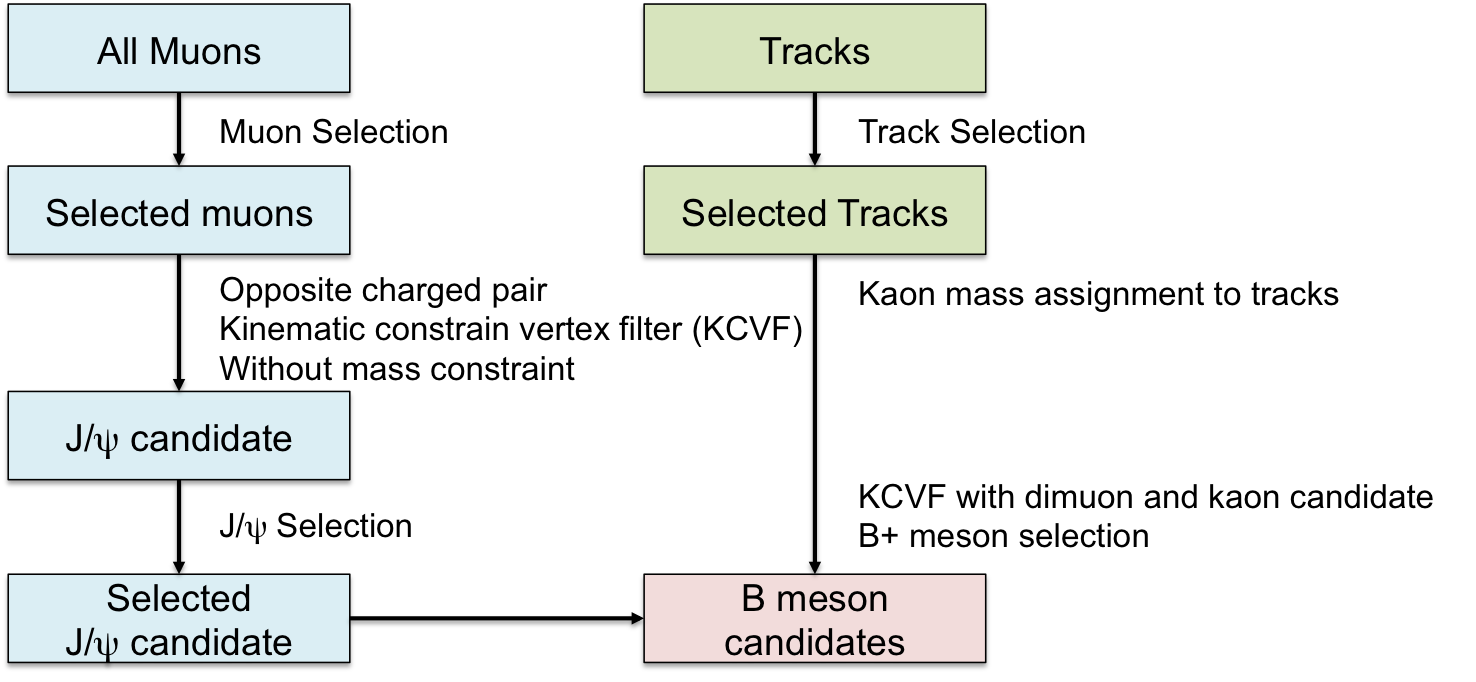
\includegraphics[width= 0.98\textwidth]{Figures/Chapter5/BPmesonWorkflow.png}
\caption{The schematic block diagram of the full reconstruction workflows for $B^+$ via the decay channel of $B^+ \rightarrow J/\psi K^+ \rightarrow \mu^+\mu^- K^+$ in the \textit{Bfinder} is shown above.}
\label{BPRECOWF}
\end{center}
\end{figure}

Here, we should note that since we do not have hadronic PID for the kaons, we assume the track to be kaons and assume the charged kaon PDG mass to the tracks \cite{AlphaTheoEx} to the tracks. Also, the invariant mass of the muon pair is constrained to the nominal $J/\psi$ meson PDG mass ($m_{J/\psi}$ = 3.096916 GeV/c$^2$) \cite{AlphaTheoEx} instead of a distribution of the dimuon mass $m_{\mu\mu}$. The output file format of \textit{Bfinder} is an Ntuple. Finally, we do not distinguish particles and anti-particles during the B-meson reconstruction. Therefore, both $B^0_s$ and $\bar{B^0_s}$ as well as $B^+$ and $B^-$ are reconstructed. Here, for simplicity, we only mention the $B^0_s$ and $B^+$ throughout the thesis. Each event will have multiple B-meson candidates \ref{BCand}.

\begin{figure}[h]
\begin{center}
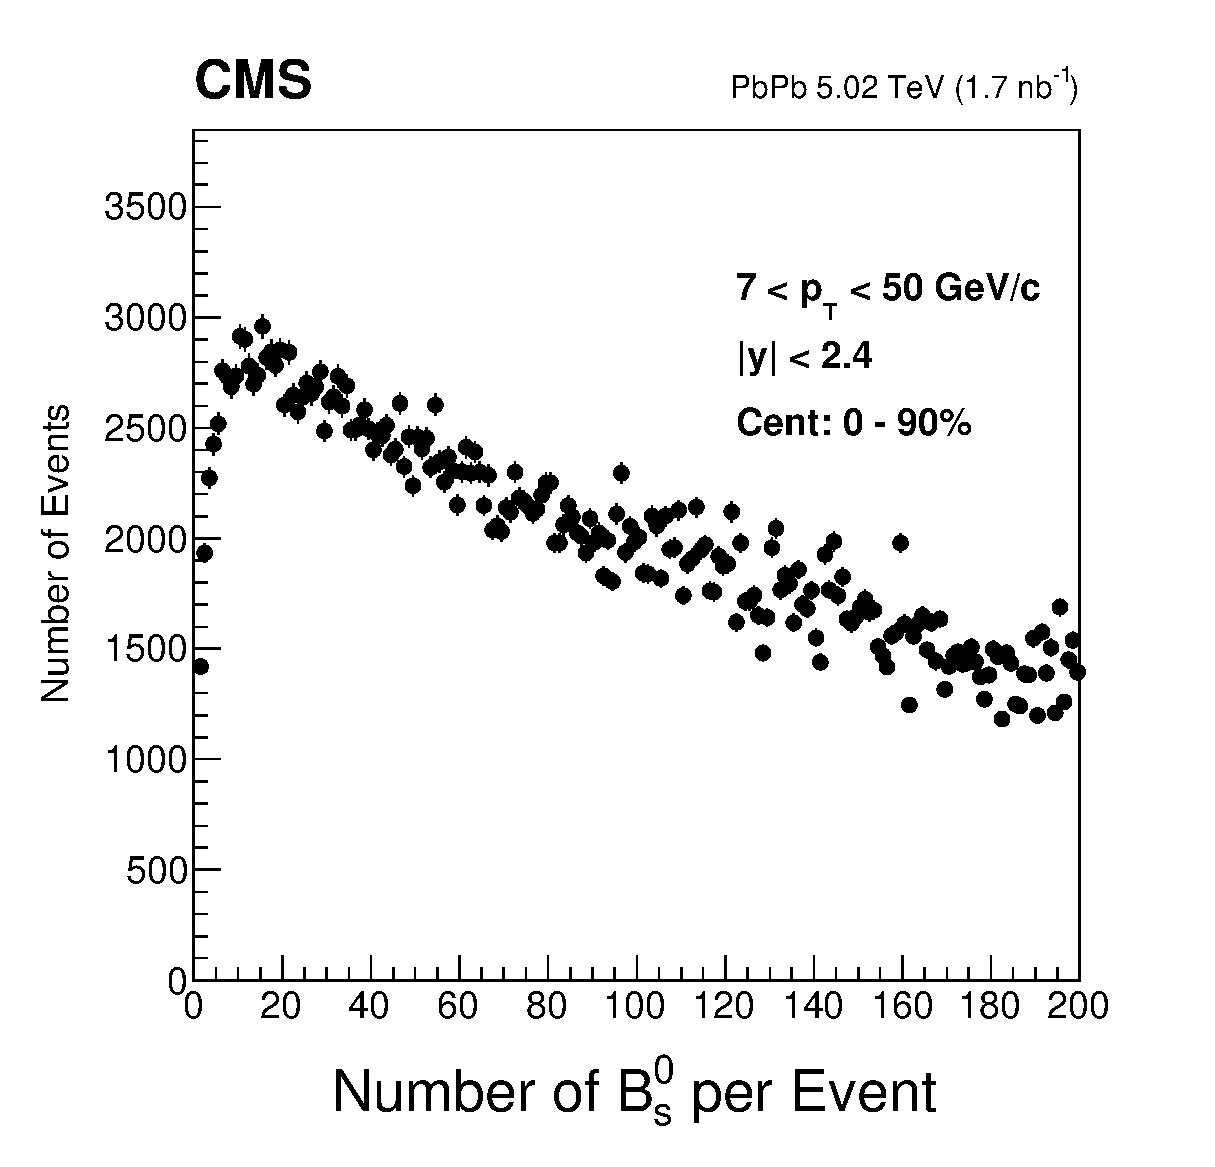
\includegraphics[width= 0.48\textwidth]{Figures/Chapter5/BsSize.eps}
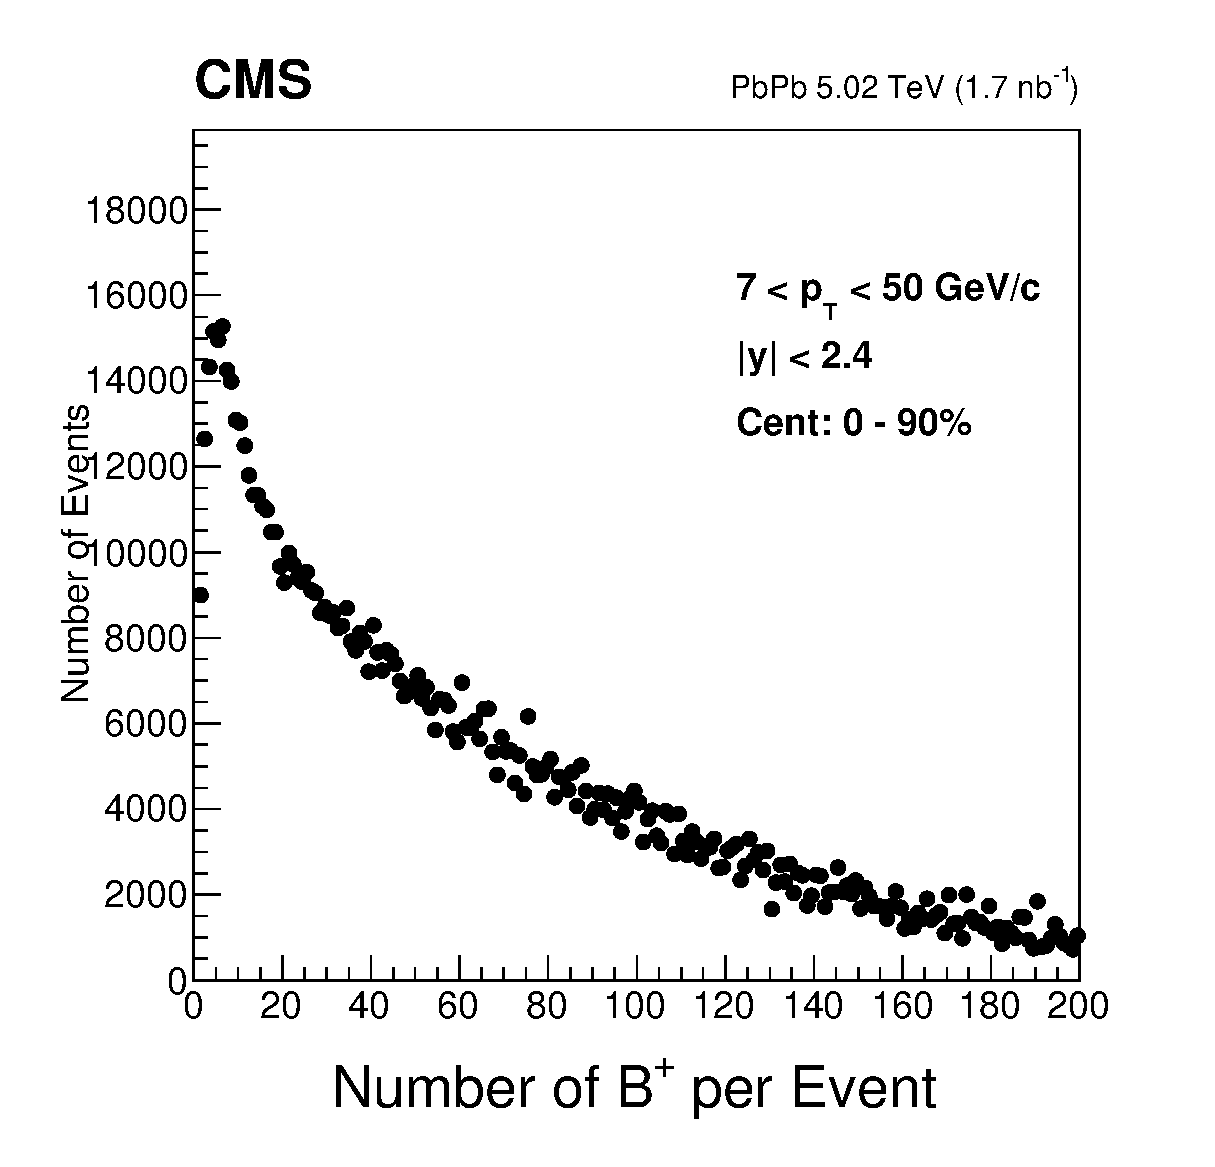
\includegraphics[width= 0.48\textwidth]{Figures/Chapter5/BPSize.eps}
\caption{The number of reconstructed B-meson candidates per event distribution in the dimuon PbPb dataset for $B^0_s$ (left) and $B^+$ (right) are shown above. Multiple B-meson candidates are reconstructed in one event.}
\label{BCand}
\end{center}
\end{figure}


Their information, including invariant mass, $p_T$, and $y$ as well as their daughter particles kinematics such as $p_T$ and $\eta$, is saved as a form of vector in each event. In this thesis, we use B-meson Ntuples to perform our analysis.


%\subsection{Decay Channels}


\subsection{Event Selections}

To ensure the quality of inelastic hadronic collisions events for B-meson reconstruct, we apply the following selections


\begin{itemize}
\item At least one reconstructed primary interaction vertex, formed by two or more tracks
\item The longitudinal distance from the center of the nominal interaction region of less than 15 cm along the beam axis: $|$PV$_{z}$$| < $ 15
\item Compatible shapes of the clusters in the pixel detector with those expected from particles produced by a PbPb collision \cite{EvtSel}
\item At least two towers in each of the HF detectors with energy deposits of more than 4GeV per tower  
\end{itemize}

\subsection{Track Selections}

In addition to event selection, we also apply track selections to improve the quality of the tracks and reject fake tracks. For $B^+$ we have the following selections

\begin{itemize}
\item General Tracks passing high purity selection (describe in section 3.4.2)
\item $|\eta| < 2.4$ and $p_T > 1$ GeV/c
\item $p_T$ momentum resolution: $\frac{\sigma_{p_T}}{p_T} < 0.1$
\item At least 10 hits in the pixel + strip tracker layers: $N_{hit} > 10$
\item (Track $\chi^2/ndf$)/(pixel + strip hits) > 0.18
\item Vertex probability > 0.05
\end{itemize}

For $B^0_s$, since we expect it to have a $\phi$ resonance in the decay chain, we require the mass of the reconstructed dikaon candidate $|p_{K^+} + p_{K^-}| = m_{KK}$ to be 0.015 GeV/c$^2$ within the $\phi$ meson PDG mass ($m_\phi$ = 1.019455 GeV/c$^2$): $|m_{KK} - m_\phi| < 0.015$ GeV/c$^2$

\subsection{Muon Selections}

The muon candidates are selected according to the \textit{hybrid-soft muon} selection, developed for the muon analysis using CMS 2012 7 TeV $pp$ data \cite{SoftMuon}. It is adapted from the soft-muon ID developed in the BPH group, with two modifications: a) the purity selection is removed, and b) the muon is required to be also \textit{global}. This selection will be updated for the one developed in 2018. The \textit{hybrid-soft muon} selection includes the following cuts:


\begin{itemize}
\item Require to be Global Muon and Tracker Muon (described in section 3.4.3)
\item At least one good muons 
\item Transverse impact parameter $D_{xy}$ < 0.3 cm
\item Longitudinal impact parameter $D_{z}$ < 20 cm
\item At least 1 muon hits on pixel tracker layers and 5 hits on both the pixel + strip tracker layers 
\end{itemize}

In addition, a muon acceptance selection to ensure the muon candidate to have a total efficiency: $\epsilon^\mu > 10\%$. Table \ref{MuonAccCut} shows acceptance cuts, designed by the CMS muon analysis group, are also applied:

\begin{table}[h]
\begin{center}
\caption{Summary table of the muon acceptance selection for muon: $|\eta^\mu|$ as a function $p_T^\mu$.}
\vspace{1em}
\label{MuonAccCut}
  \begin{tabular}{ |c | c| c| c|}
    \hline 
Centrality &  $\langle N_{part} \rangle$ &$\langle N_{coll} \rangle$  & $\langle T_{AA} \rangle$  \\
     \hline
         \hline
 $|\eta^\mu|$ & 0 -- 1.2   & 1.2 -- 2.1  &  2.1 -- 2.4   \\
$p_T^\mu$ (GeV/c) &  > 3.5 &  > 5.47 - 1.89 & $\eta$  > 1.5   \\
     \hline
    \hline
\end{tabular}
\end{center}
\end{table}

Table \ref{MuonAccCut} comes from the muon analysis in the 2018 PbPb dataset. Figure \ref{MuonAccPlot} shows the muon reconstruction, identification, and trigger efficiency as a function of $p_T^\mu$ and $\eta^{\mu}$ \cite{MuonAccRef}

\begin{figure}[h]
\begin{center}
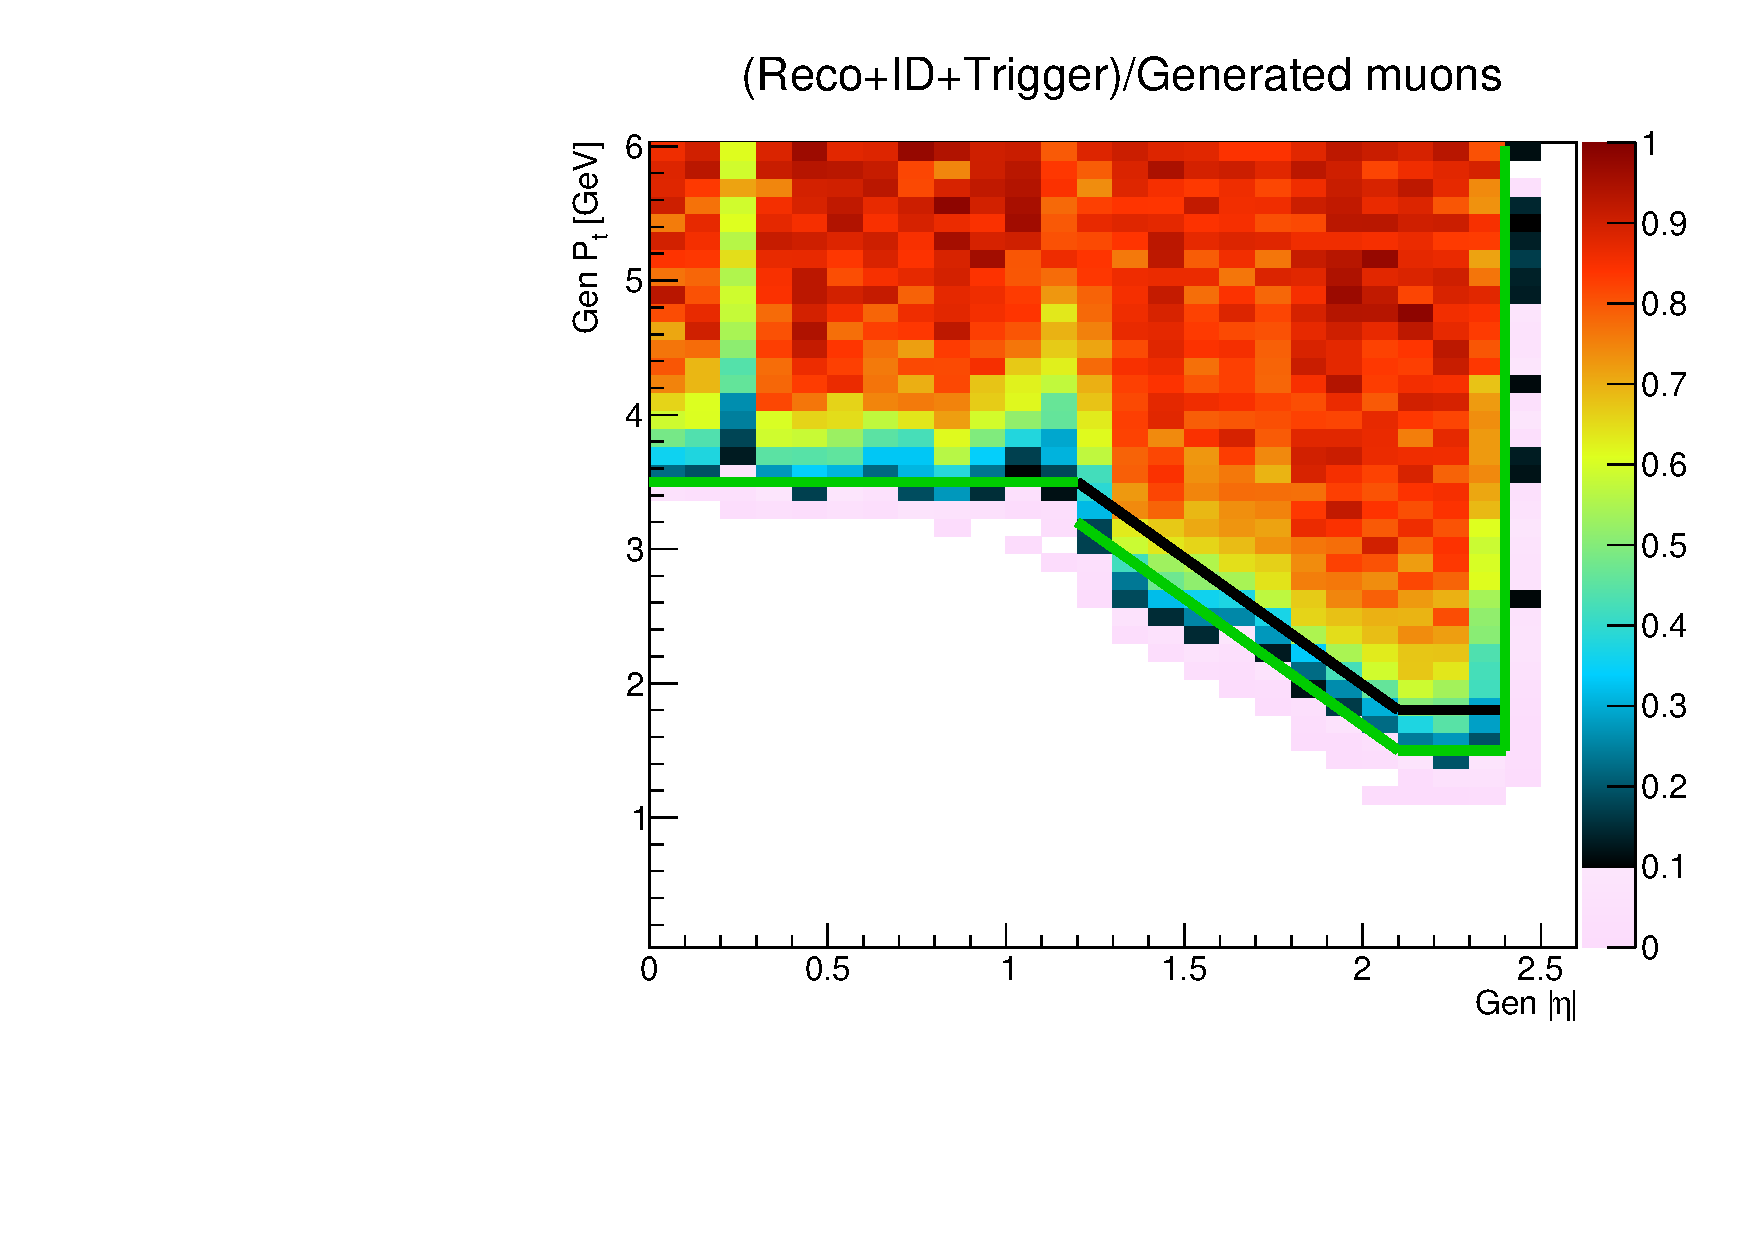
\includegraphics[width= 0.48\textwidth]{Figures/Chapter5/MuonAccPbPb.pdf}
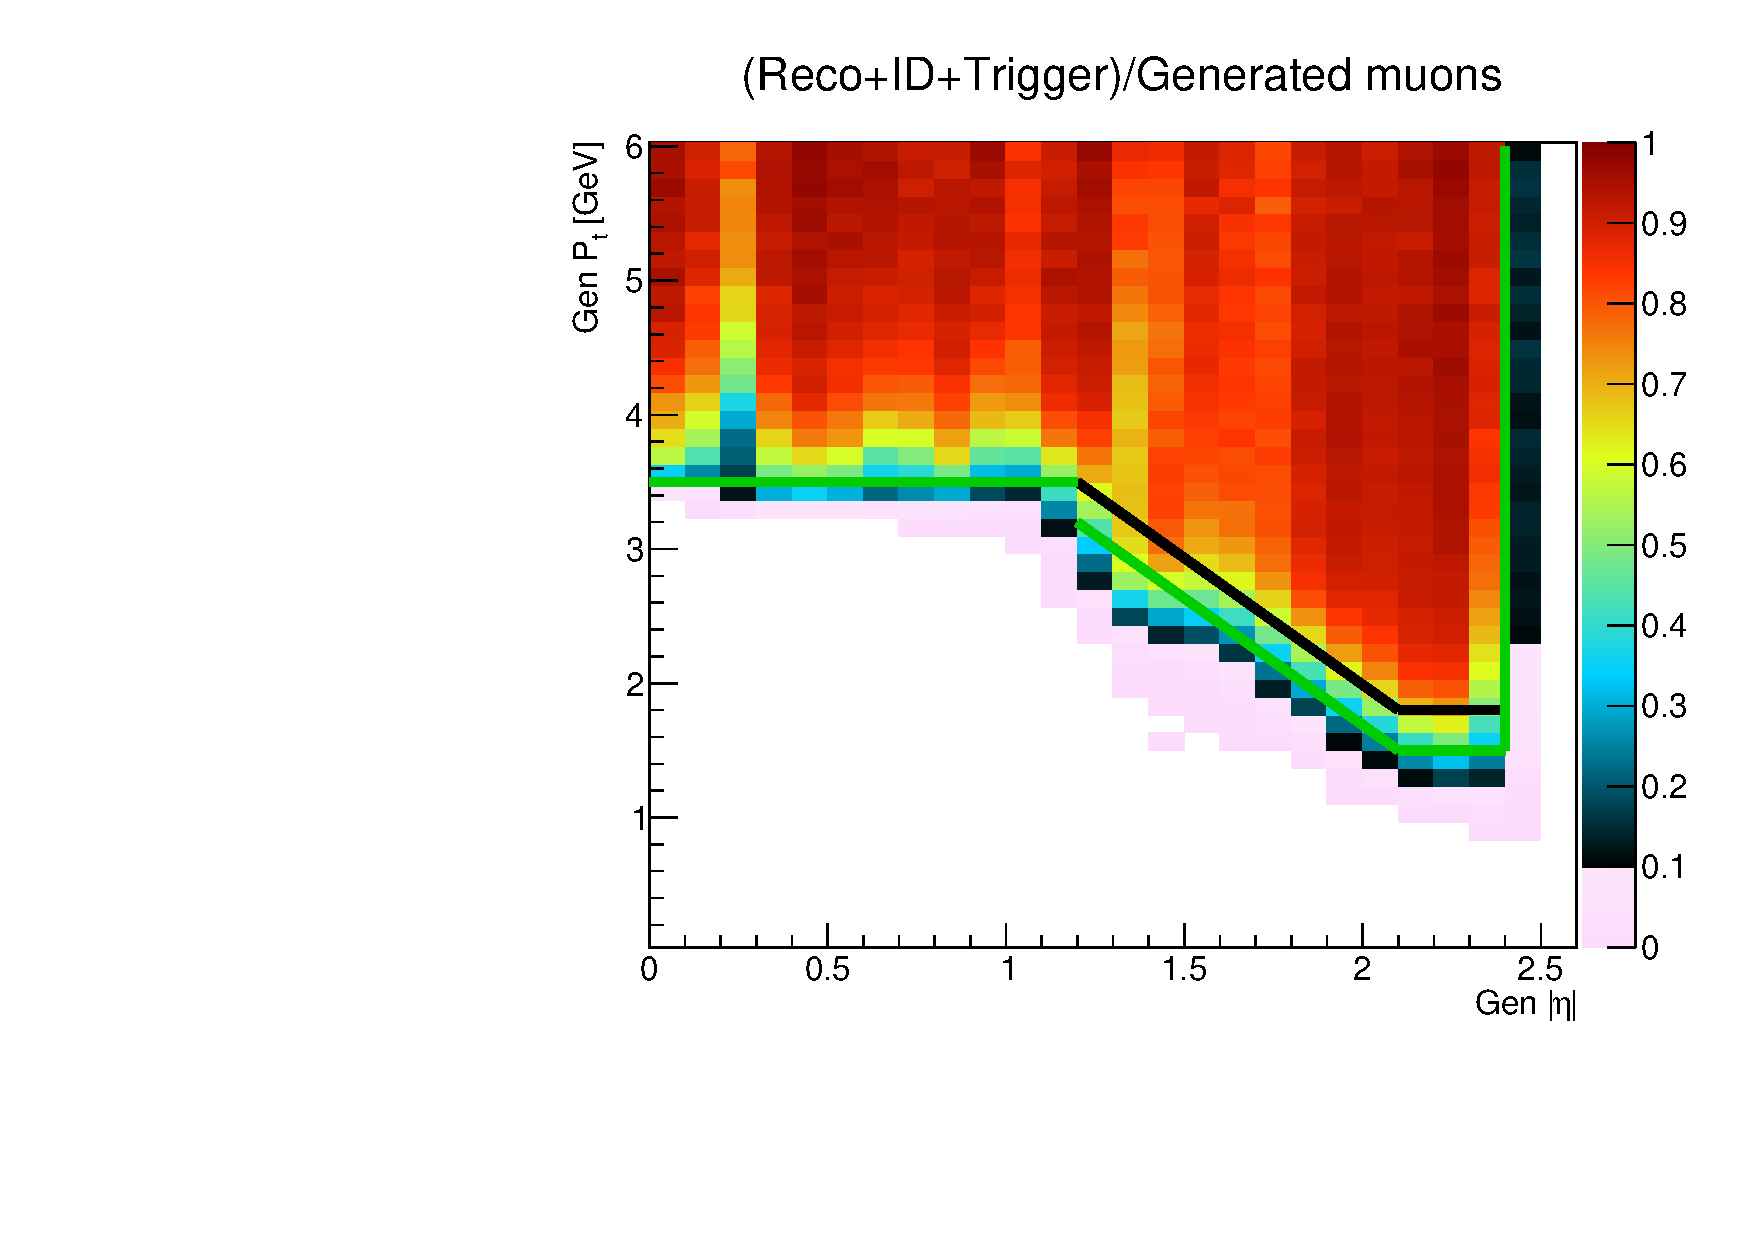
\includegraphics[width= 0.48\textwidth]{Figures/Chapter5/MuonAccPP.pdf}
\caption{The total efficiency, including reconstruction, identification, and trigger, of a single muon in 2018 PbPb (left) and 2017 $pp$ (right) are shown above. The black curve is the 2015 PbPb and $pp$ 90\% muon efficiency boundary while the green curve is the 2017 $pp$ and 2018 PbPb 90\% muon efficiency boundary. The green boundary is translated to numerical values in Table \ref{MuonAccCut}}
\label{MuonAccPlot}
\end{center}
\end{figure}

We should note that there is a discontinuity of the muon acceptance selection at $|\eta| = 1.2$. Aside from the single muon selections, the following selections are applied to the reconstructed dimuon candidates


\begin{itemize}
\item Two muons have opposite charges 
\item Two muons are tracker muons
\item Dimuon invariant mass about 0.15 GeV/c$^2$ near the $J/\psi$ PDG mass ($m_{J/\psi}$ = 3.096916 GeV/c$^2$): $|m_{\mu\mu} - m_{J/\psi}| < 0.15$ GeV/c$^2$
\item One muon is L2 muon and the other one is L3 muon (described in section 2.25)
\item Probability of the two muon tracks to originate from the same decay vertex $>$ 1\%
\end{itemize}


In addition, a B-meson invariant mass window of $4 < m_B < 6$ GeV/c$^2$ is applied since the $B^0_s$ mass is $m_{B^0_s} = $ 5.367 GeV/c$^2$ and the $B^0_s$ mass is $m_{B^+} = $ 5,279 GeV/c$^2$ \cite{AlphaTheoEx}. Anything far away from the mass window should not be considered. After applying all these preliminary selections to improve the quality of our dataset for the analysis, we are ready to perform cut optimization to further reject background candidates based on the decay topology of the $B^0_s$ and $B^+$ decay chains.


\section{Cut Optimization} 


Given the high combinatorial background, particularly in PbPb collision where we have thousands of tracks per event \cite{PbPbMulti}, it is not possible to observe B-meson resonance by simply applying the preselection presented in the previous section. Figure \ref{BMassPreCut} shows the invariant mass distribution of fully reconstructed $B^0_s$ and $B^+$ at $7 < p_T < 50$ GeV/c after the event, track, and muon selections.

\begin{figure}[h]
\begin{center}
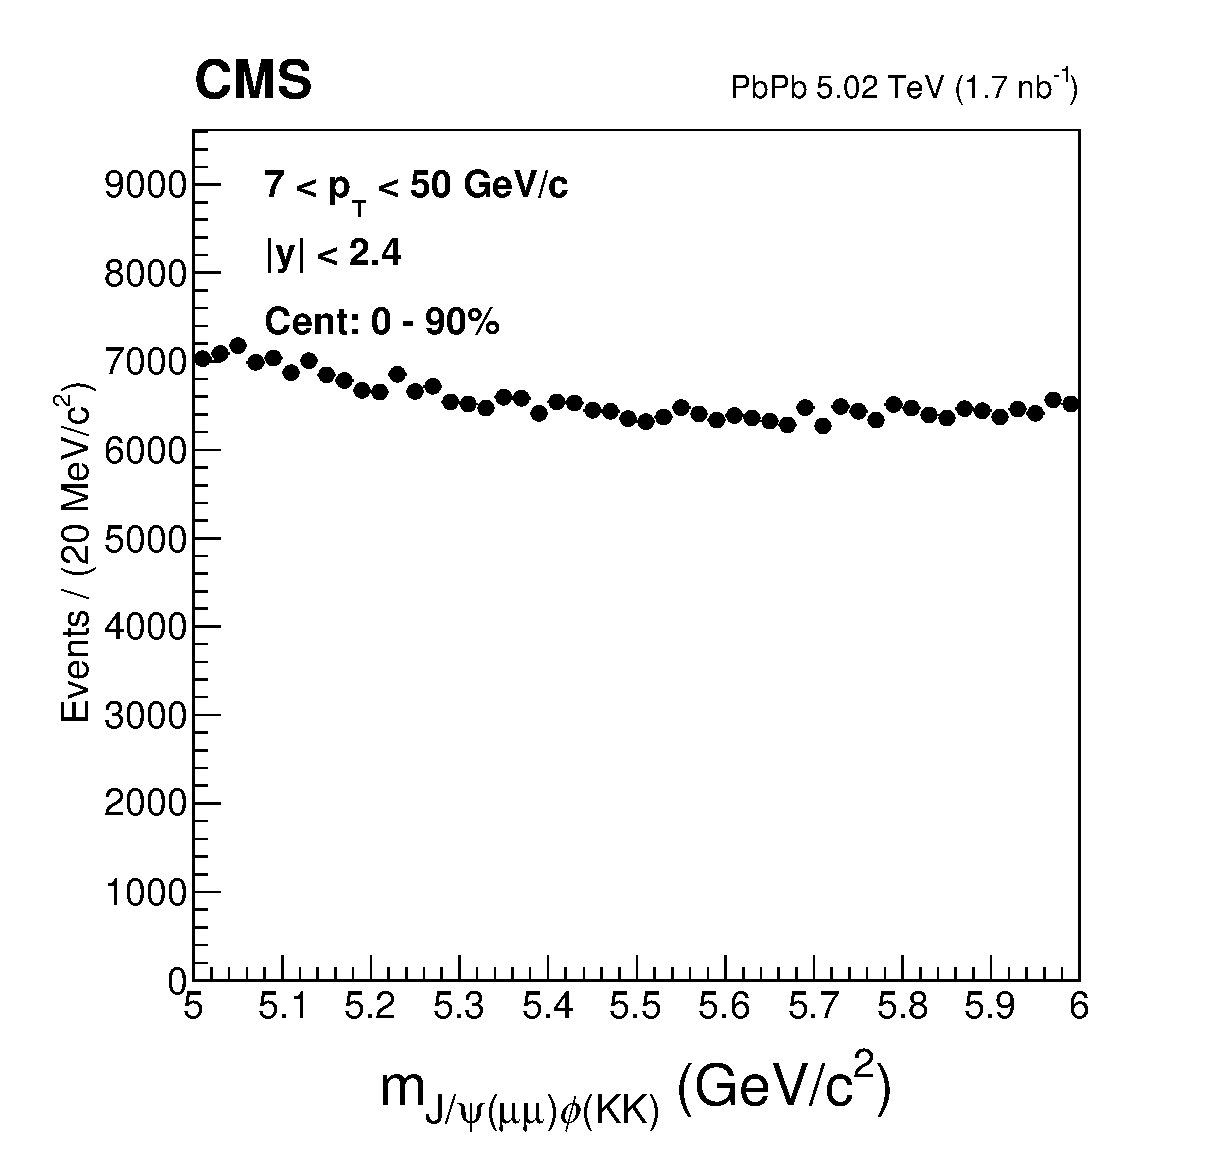
\includegraphics[width= 0.48\textwidth]{Figures/Chapter5/BsMassPreCut.eps}
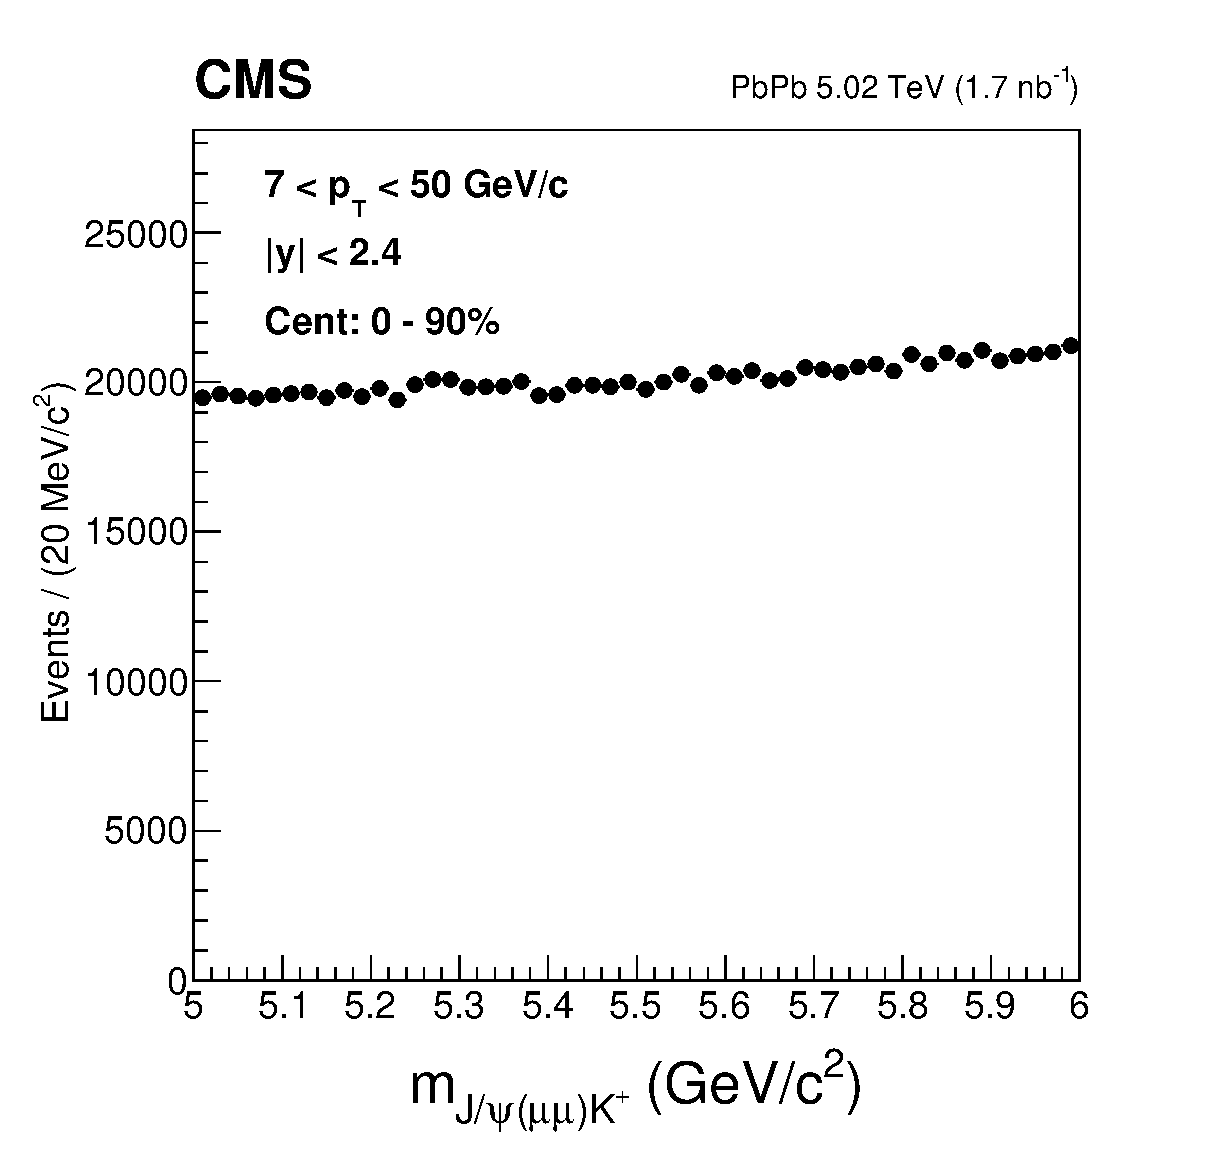
\includegraphics[width= 0.48\textwidth]{Figures/Chapter5/BPMassPreCut.eps}
\caption{The invariant mass distributions of fully reconstructed $B^0_s$ (left) and $B^+$ (right) after preselection are shown above.}
\label{BMassPreCut}
\end{center}
\end{figure}


No B-meson signal is observed in the data. Therefore, aside from the preselections, a multivariate analysis (MVA) approach \cite{MVARef} is thus conducted in order to develop an optimal selection to separate signal B mesons from the background and reconstruct a significant resonance in the invariant mass distribution in the data. The fitting performance is further related to both the amount of signal and background presented in the mass spectrum. 


\subsection{Topological Variables}


By an MVA analysis, one can then find the proper selection criteria which is optimized for this purpose. Several variables related to kaon tracks and B mesons decay topology are applied in order to reduce the combinatorial background that arises from a random combination of tracks and muons. The topological variables used in B-meson analyses to be optimized by  are listed as follows:

\textbf{Topological Variables for $B^0_s$:}
\begin{itemize}
\item Kaon track $p_T$
\item Kaon track transverse distance to closest approach (DCA) significance: $DCA_{xy}/\sigma_{DCA_{xy}}$ 
\item Kaon track longitudinal distance to closest approach (DCA) significance: $DCA_{z}/\sigma_{DCA_{z}}$
\item Dikaon invariant mass distance to the $\phi$ meson PDG mass: $|m_{KK} - m_{\phi}|$
\item The $B^0_s$ meson decay length [or the distance between primary vertex (PV) and secondary vertex (SV)] significance: $|\vec{D}(SV,DV)|/|\sigma_{\vec{D}(SV,DV)}|$
\item The open angle between the B-meson decay length vector and its three momentum: $\alpha: \cos(\alpha) = \frac{\vec{D}(SV,DV) \cdot \vec{p}}{|\vec{D}(SV,DV)||\vec{p}|}$
\item The cosine angle of the opening angle in the transverse direction:  $\theta_B: \cos(\theta_B) = \frac{\vec{D(SV,DV)_{xy} \cdot \vec{p_T}}}{|\vec{D(SV,DV)_{xy}}||\vec{p_T}|}$
\item Vertex fitting probability: the $\chi^2$ value of the vertex fitting
\end{itemize}

For $B^+$, we also apply some addition rectangular selections before cut optimization

\textbf{Topological Variables for $B^+$:}
\begin{itemize}
\item Kaon track $p_T$
\item Kaon track $|\eta|$
\item Kaon track transverse distance to closest approach (DCA) significance: $DCA_{xy}/\sigma_{DCA_{xy}}$ 
\item The $B^+$ meson decay length [or the distance between primary vertex (PV) and secondary vertex (SV)] significance: $|\vec{D}(SV,DV)|/|\sigma_{\vec{D}(SV,DV)}|$
\item The open angle between the B-meson decay length vector and its three momentum: $\alpha: \cos(\alpha) = \frac{\vec{D}(SV,DV) \cdot \vec{p}}{|\vec{D}(SV,DV)||\vec{p}|}$
\item The cosine angle of the opening angle in the transverse direction:  $\theta_B: \cos(\theta_B) = \frac{\vec{D(SV,DV)_{xy} \cdot \vec{p_T}}}{|\vec{D(SV,DV)_{xy}}||\vec{p_T}|}$
\item Vertex fitting probability: the $\chi^2$ value of the vertex fitting
\end{itemize}

Figure \ref{DecayTopoBs} and \ref{DecayTopoBP} show the definition of topological variables of $B^0_s$ and $B^+$ decay chains respectfully 

\begin{figure}[h]
\begin{center}
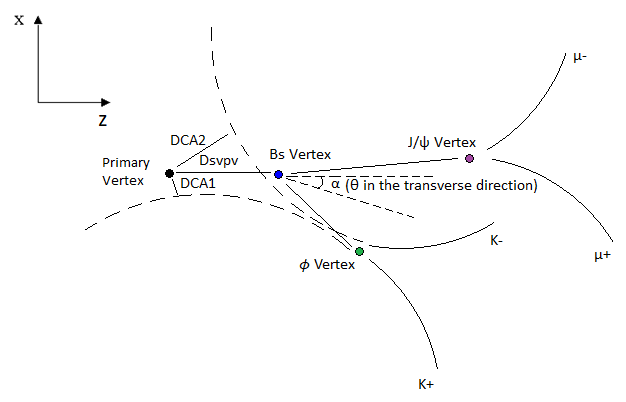
\includegraphics[width= 0.98\textwidth]{Figures/Chapter5/BsDecay.png}
\caption{The definition of topological variables in the decay of $B^0_s \rightarrow J/\psi \phi \rightarrow \mu^+\mu^- K^+K^-$ (left) are schematically shown above.}
\label{DecayTopoBs}
\end{center}
\end{figure}


\begin{figure}[h]
\begin{center}
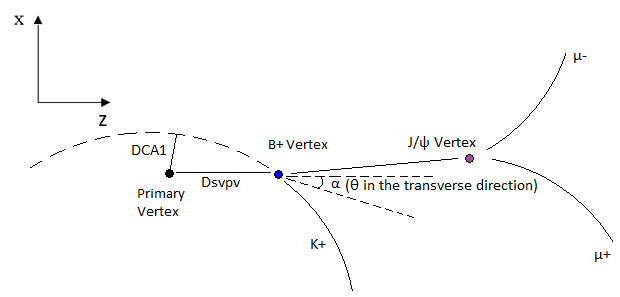
\includegraphics[width= 0.98\textwidth]{Figures/Chapter5/BPDecay.png}
\caption{The definition of topological variables in the decay of $B^+ \rightarrow J/\psi K^+ \rightarrow \mu^+\mu^- K^+ $ are schematically shown above.}
\label{DecayTopoBP}
\end{center}
\end{figure}

These topological variables will become the inputs to the multivariate analysis to optimize the signal significance.

\subsection{Multivariate Analysis}

In statistics, many data analysis techniques only focus on one or two variables individually. Multivariate analysis (MVA) analyzes more than two variables simultaneously to improve the data analysis. Figure \ref{MVADemo} shows schematically the advantages of MVA to traditional statistical techniques in data analysis to separate the signal from the background with two variables. 




\begin{figure}[h]
\begin{center}
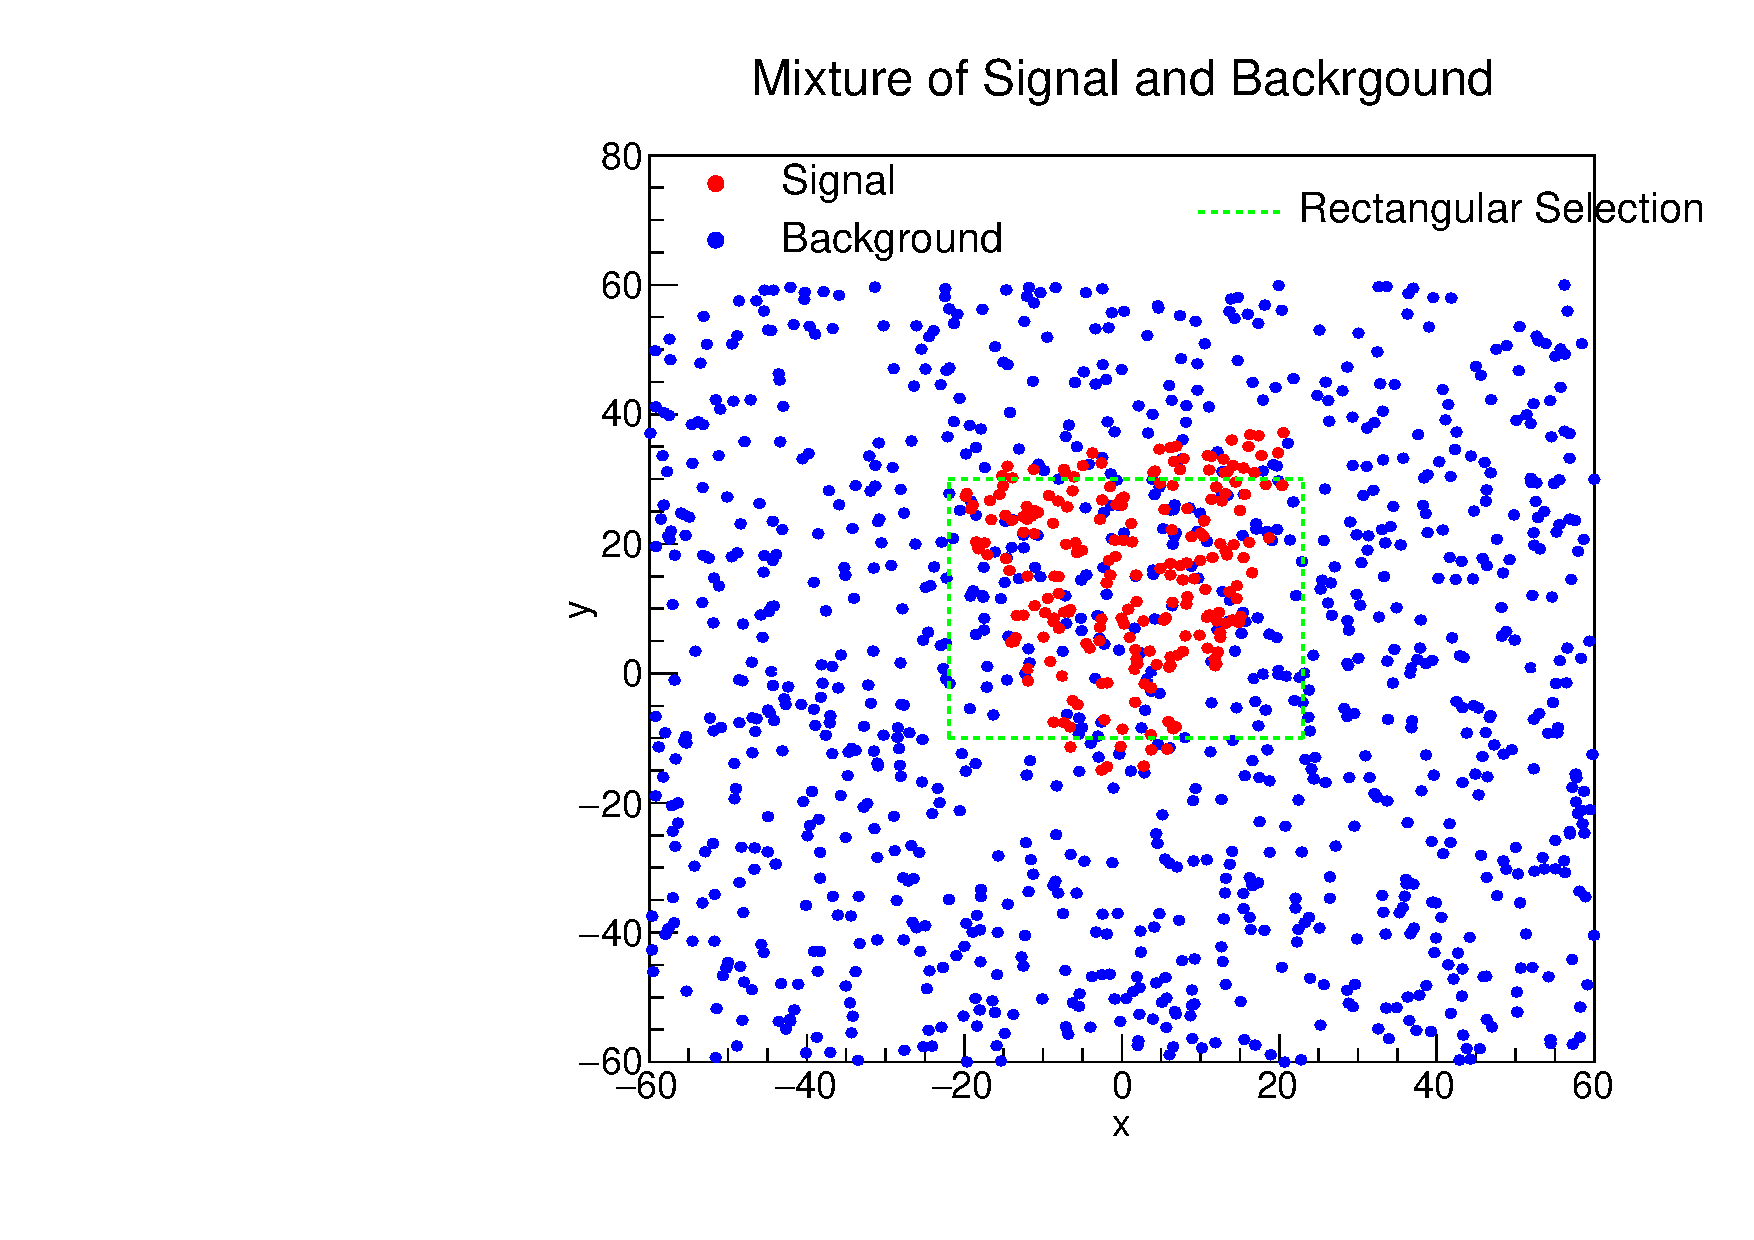
\includegraphics[width= 0.48\textwidth]{Figures/Chapter5/Rectangular.pdf}
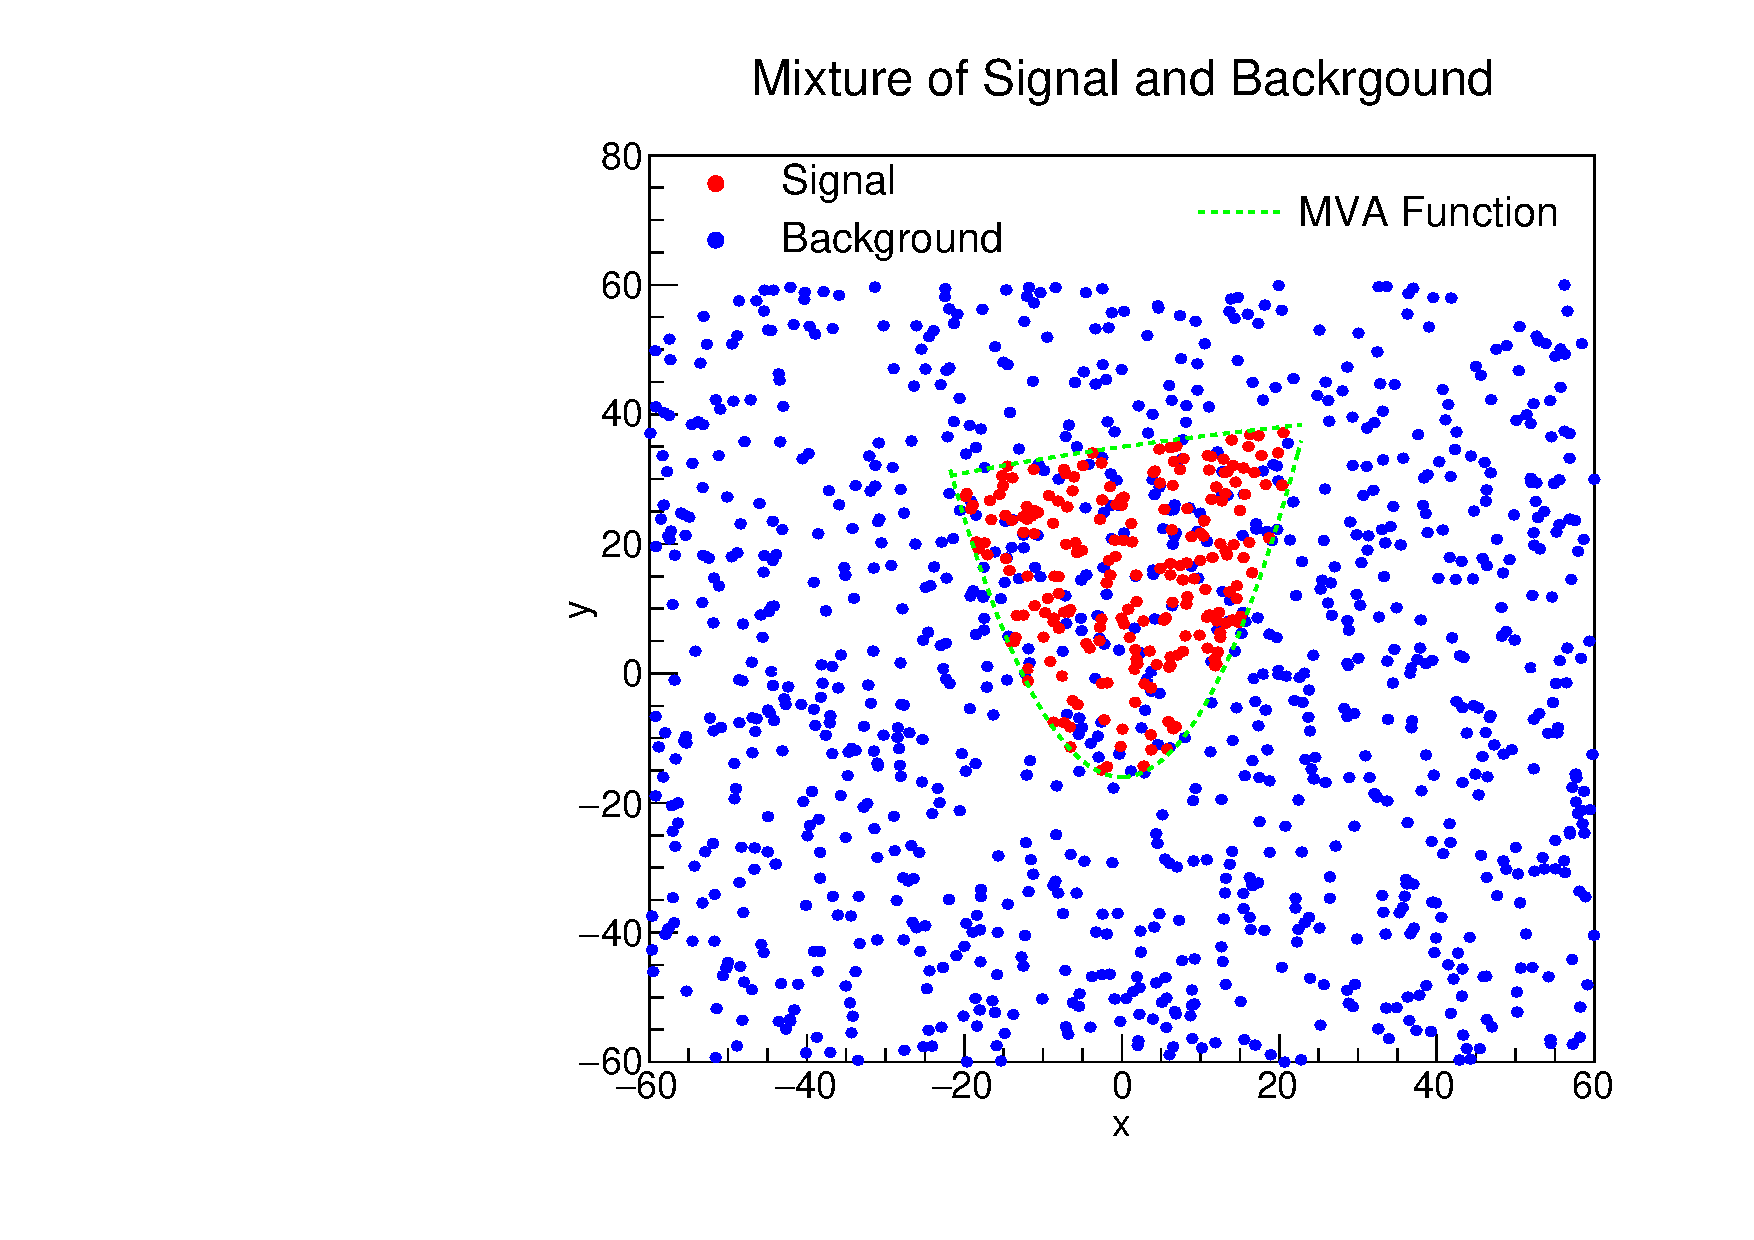
\includegraphics[width= 0.48\textwidth]{Figures/Chapter5/MVA.pdf}
\caption{The performance of traditional rectangular selection with a range of $x$ and $y$ (left) compared to the MVA method of a curve as a function of X and Y (right) are shown above. Here, we have the total signal S = 215 and the background B =  1000.}
\label{MVADemo}
\end{center}
\end{figure}

We can see that in multivariate analysis, an MVA value as a function of two independent variables $x$ and $y$: $MVA = f(x,y)$ is able to select signal out from the background with higher purity (larger S/B ratio) than the rectangular selection function $x_1 < x < x_2$ and $y_1 < y < y_2$. Table \ref{MVAvsRec} shows the performance of MVA and traditional rectangular selections

\begin{table}[h]
\begin{center}
\caption{The numerical values of comparison between the traditional rectangular selections and MVA.}
\vspace{1em}
\label{MVAvsRec}
  \begin{tabular}{ |c | c| c| c|}
    \hline 
Analysis Techniques &  S & B & S/B \\
     \hline
Rectangular & 174 & 135 & 1.29  \\
         \hline
MVA &   215  & 114  & 1.89  \\
     \hline
    \hline
\end{tabular}
\end{center}
\end{table}


\subsection{Machine Learning Techniques}

Machine learning, as a branch of artificial intelligence, is the science that gets computers to learn what human beings do. It is an automating data analysis method for the model building to solve practical problems. Figure \ref{MLProblem} demonstrates the data analysis problems including classification, regression, and clustering, where machine learning could be applied.

\begin{figure}[h]
\begin{center}
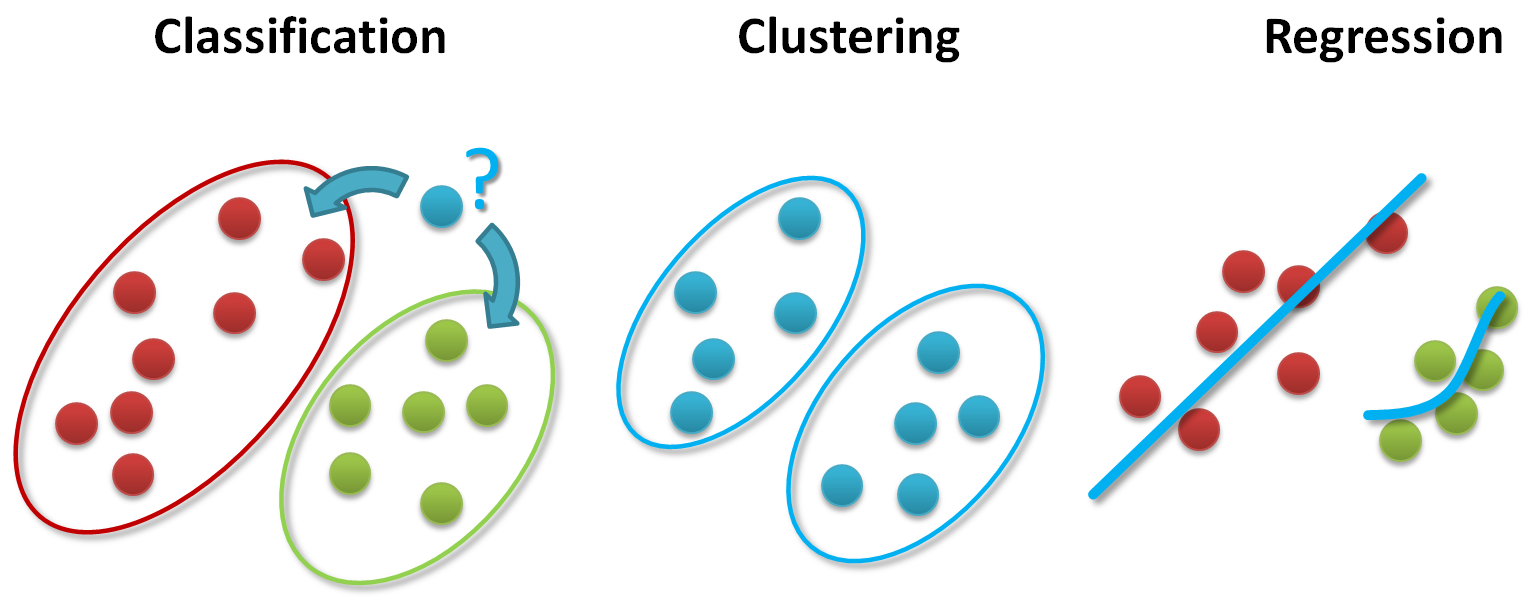
\includegraphics[width= 0.85\textwidth]{Figures/Chapter5/MLProblemsNew.png}
\caption{The solutions to classification, regression, and clustering problems with supervised and unsupervised machine learning approaches are shown schematically above.}
\label{MLProblem}
\end{center}
\end{figure}

In this analysis, our goal is to separate B-meson signal out of the background. Therefore, it is a classification problem. Therefore, machine learning can be a powerful tool to solve our problems. We apply supervised machine learning to train the computer and let them find the optimal selections for B-meson analyses.   


\subsection{Terminologies}

The following list explains the technical jargon of machine learning techniques along with MVA that may be mentioned later in this thesis:


\begin{itemize}
\item \textbf{Training samples:} the input samples including both background and signal to train the computer. In this thesis, we use the B mesons candidates coming from our chosen B-meson decay channels (GEN Matched) in MC as the signal input and the B mesons candidates from the invariant mass sideband region with a distance of greater than 0.2 GeV/c$^{2}$ to the PDG mass of B mesons as background input to the \textit{TMVA} 
\item \textbf{Testing samples:} the samples including both background and signal going to be tested with the output from the training. The testing sample should not be the same as the training sample.
\item \textbf{Correlation matrix:} the linear correlation between the input variables for training 
\item \textbf{ROC curve:} the curve of signal efficiency as a function of the background rejection (= 1 $-$ background efficiency) for a given MVA value. Here the efficiency is defined as: efficiency = the number of candidates with the given MVA cut/ number of candidates without the MVA cut.
\item \textbf{Overtraining:} A Kolmogorov-Smirnov test \cite{KSTest} to compare the shape of the MVA distributions of training and test samples. It returns probabilities for both signal and background between 0 and 1. The closer to 0, the poor the matching, the more the overtraining will be.  
\end{itemize}


Figure \ref{SigBackRegion} shows the definition of signal and background regions in $B^0_s$ and $B^+$ invariant mass plot. 

\begin{figure}[h]
\begin{center}
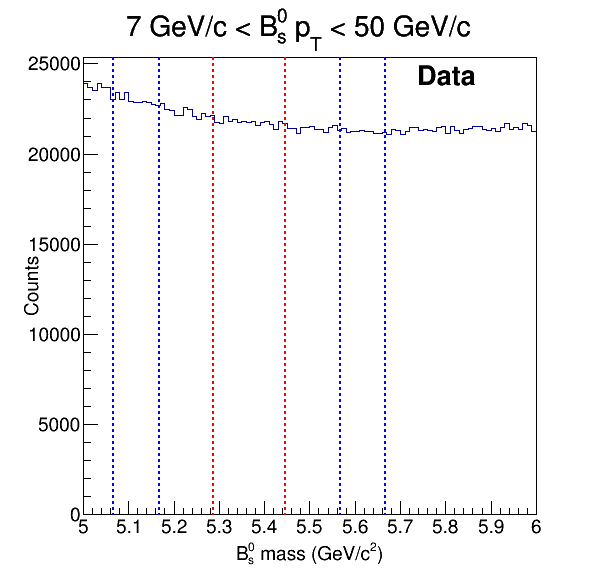
\includegraphics[width= 0.48\textwidth]{Figures/Chapter5/BsData.png}
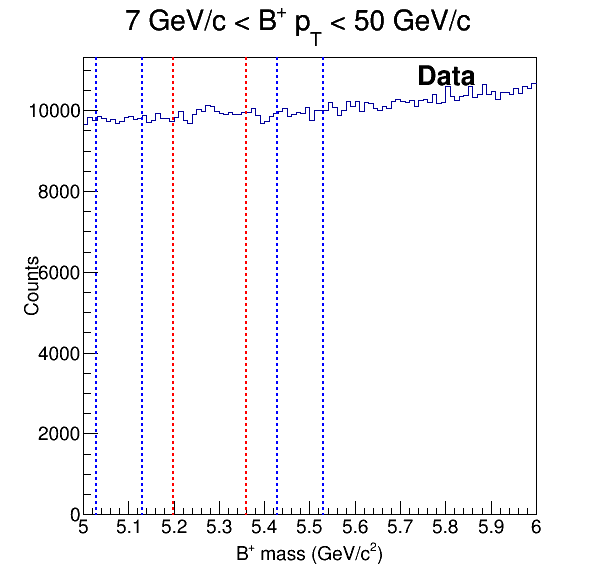
\includegraphics[width= 0.48\textwidth]{Figures/Chapter5/BPData.png}
\caption{The definitions of signal (red band) and background region (blue band) in the fully reconstructed B-meson invariant distribution for $B^0_s$ (left) and $B^+$ (right) are shown above.}
\label{SigBackRegion}
\end{center}
\end{figure}

The signal region is $|m_B - m_B^{PDG}| < 0.08$ GeV/c and the background region is $0.20 < |m_B - m_B^{PDG}| < 0.30$ GeV/c$^2$ for $B^0_s$ and $0.15 < |m_B - m_B^{PDG}| < 0.25$ GeV/c$^2$  for $B^+$.


\subsection{Boosted Decision Tree Algorithm}

Nowadays, machining learning has become sophisticated. There are many well developed machining learning algorithms such as Rectangular Cut (CutsSA) Linear Discriminant (LD), Boosted Decision Tree (BDT), neutral network feed-forward Multilayer Perceptrons with recommended ANN with BFGS training method and bayesian regulator (MLPBNN), and Deep Learning in the market. Here, I will give a brief introduction about the BDT algorithm in terms of \textit{Boosted} and \textit{Decision Tree}

\textbf{Boosted:} Boosted here refers to the ``boosting'' factor $\alpha$ in the hypothesis function to let the machine learn and correctly model the actual curve \cite{BoostingRef}. According to supervised machine learning, in order to use the boosting method, we first assign an ensemble of many weak learners to create a strong learner. The idea of boosting is to keep reweighing the function to enhance the classification and regression and performance by applying an MVA algorithm subsequently to the reweighed version of the training data in a sequential matter. Eventually, the hypothesis will converge a function that can describe the actual data. Figure \ref{Boosting} below shows schematically the boosting scheme 


\begin{figure}[h]
\begin{center}
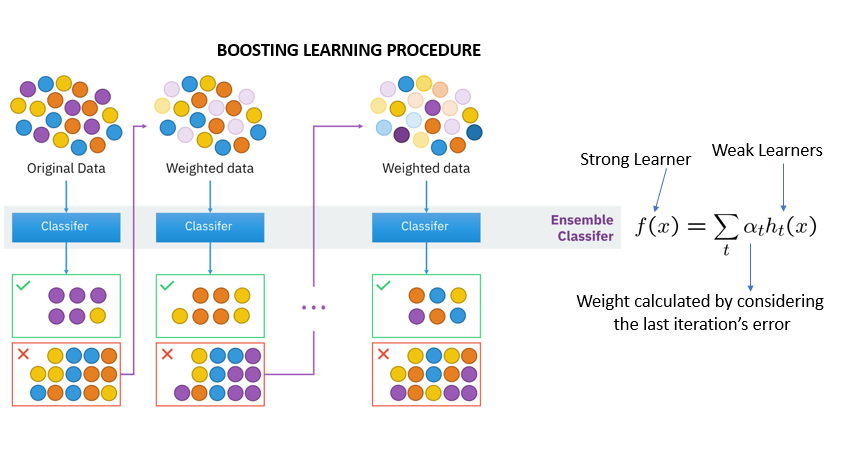
\includegraphics[width= 0.85\textwidth]{Figures/Chapter5/Boosting.jpg}
\caption{The schematic illustration of boosting procedures in machine learning is shown above.}
\label{Boosting}
\end{center}
\end{figure}


\textbf{Decision Tree:} A decision tree, sometimes called a regression tree, is a binary decision support tool using a tree-like model of decisions and list their possible consequences. Starting from a sample to analyze, it sets up criteria for selections to decide the likelihood of signal and background based on the pure signal and background input samples. Then, it makes binary decisions (Yes/No), in each branch to select a subset of samples out of the current sample, can be sequentially or in parallel. It will then iterate multiple times until the subsamples are considered as signal or background. In TMVA machinery, the number of iteration is called \textit{NTree}. Figure \ref{DecisionTree} is a schematic demonstration of a decision tree with NTree = 4

\begin{figure}[h]
\begin{center}
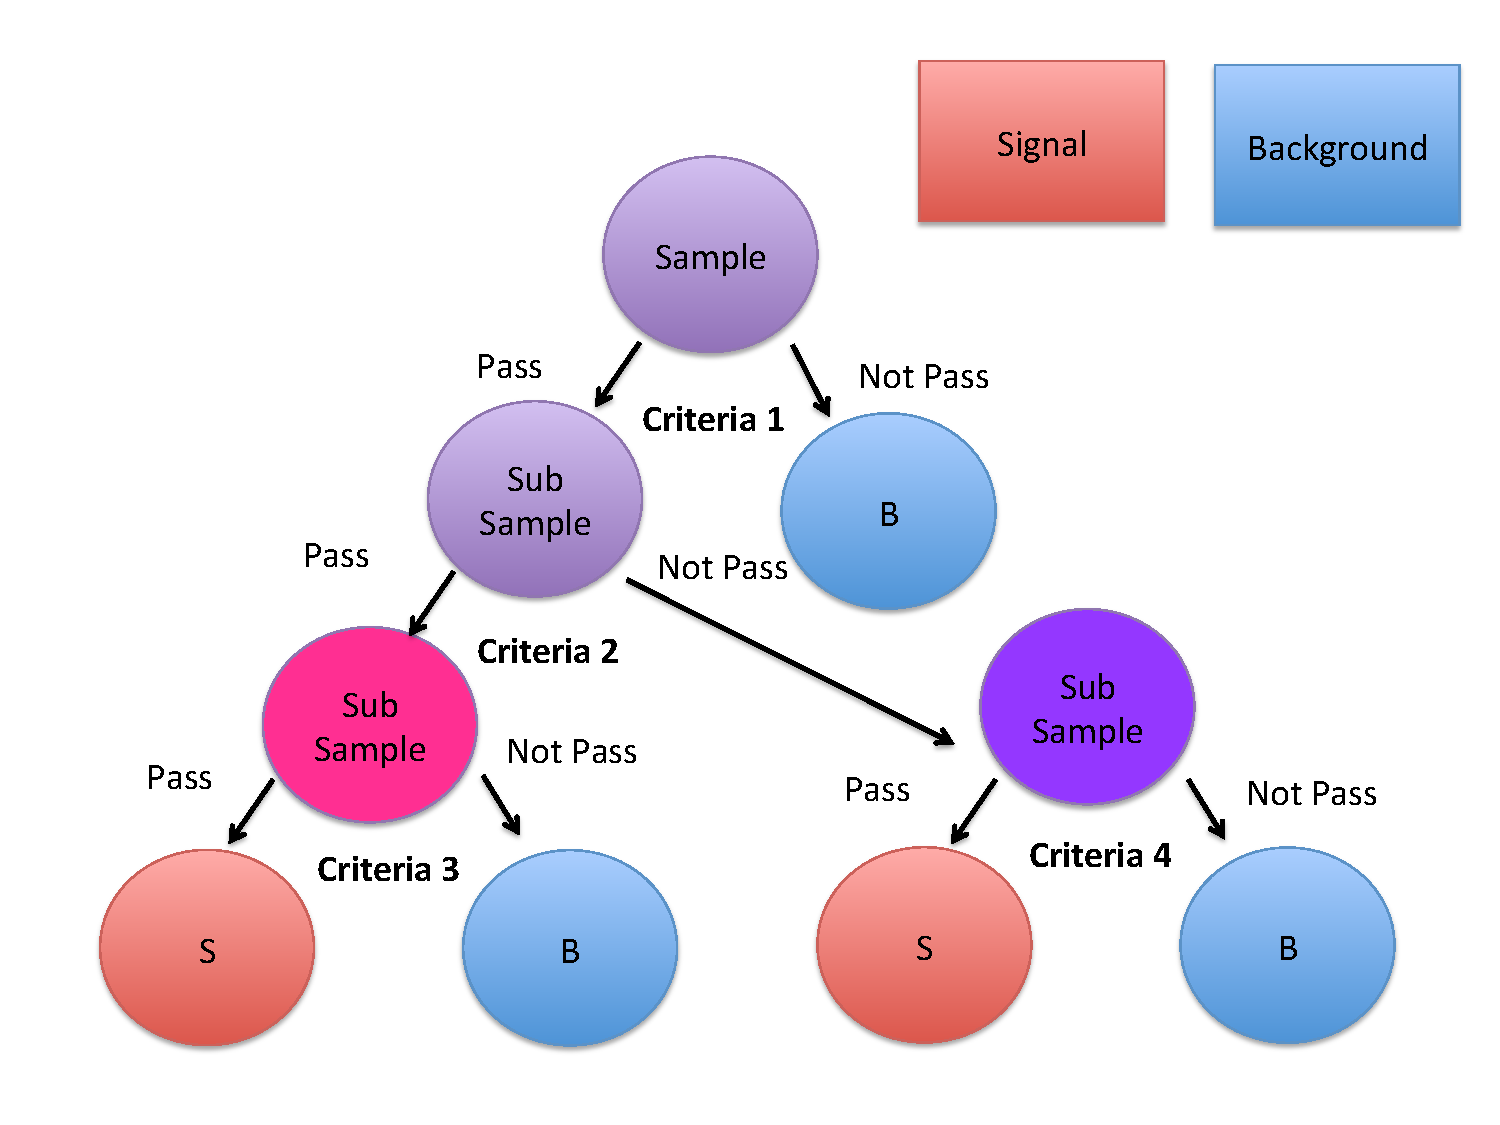
\includegraphics[width= 0.85\textwidth]{Figures/Chapter5/DecisionTree.pdf}
\caption{The schematic block diagram of a binary decision tree with NTree = 4 to separate signal and background in a training sample.}
\label{DecisionTree}
\end{center}
\end{figure}

In general, the performance of BDT will improve as NTree become larger. However, we should note that normally NTree is required to be smaller than the sample statistics. Otherwise, overtraining may occur and could induce biases in the data analysis. We should note that the BDT score range from -1 to 1. 



\subsection{TMVA Training}


To perform machine learning, I use the Toolkit for Multivariate Data Analysis with ROOT (\textit{TMVA}) \cite{TMVA}, a dedicated ROOT base machine learning software framework on C++ programing language, to train the computer to find the optimal MVA value as a function of the topological variables in our B-meson analyses. We propose to optimize $B^0_s$ in the $p_T$ binning of [7, 10, 15, 20, 50] GeV/c and $B^+$ in the $p_T$ binning of [5, 7, 10, 15, 20, 30, 40, 50, 60] individually. The following procedures are carried out:

Step 1: identify sufficient signal and background samples to train the computer within \textit{TMVA} machinery. 

Step 2: choose the training algorithms to use. Here, we choose CutsSA, CutsGA, BDT, MLP, and MLPBNN2 algorithms

Step 3: decide the training parameters for each training algorithm. 

Step 4: run the TMVA machinery and generate the performance plots 

Step 5: choose the best algorithm according to the performance


\subsection{Training Performance}

After finishing the TMVA training procedure, we are ready to look at the training performance. First, we the correlation between the input topological variables. Figure \ref{CorrMatrix} shows the correlation matrices of $B^0_s$ and $B^+$ topological variables for B-meson $10 < p_T < 15$ GeV/c.

\begin{figure}[h]
\begin{center}
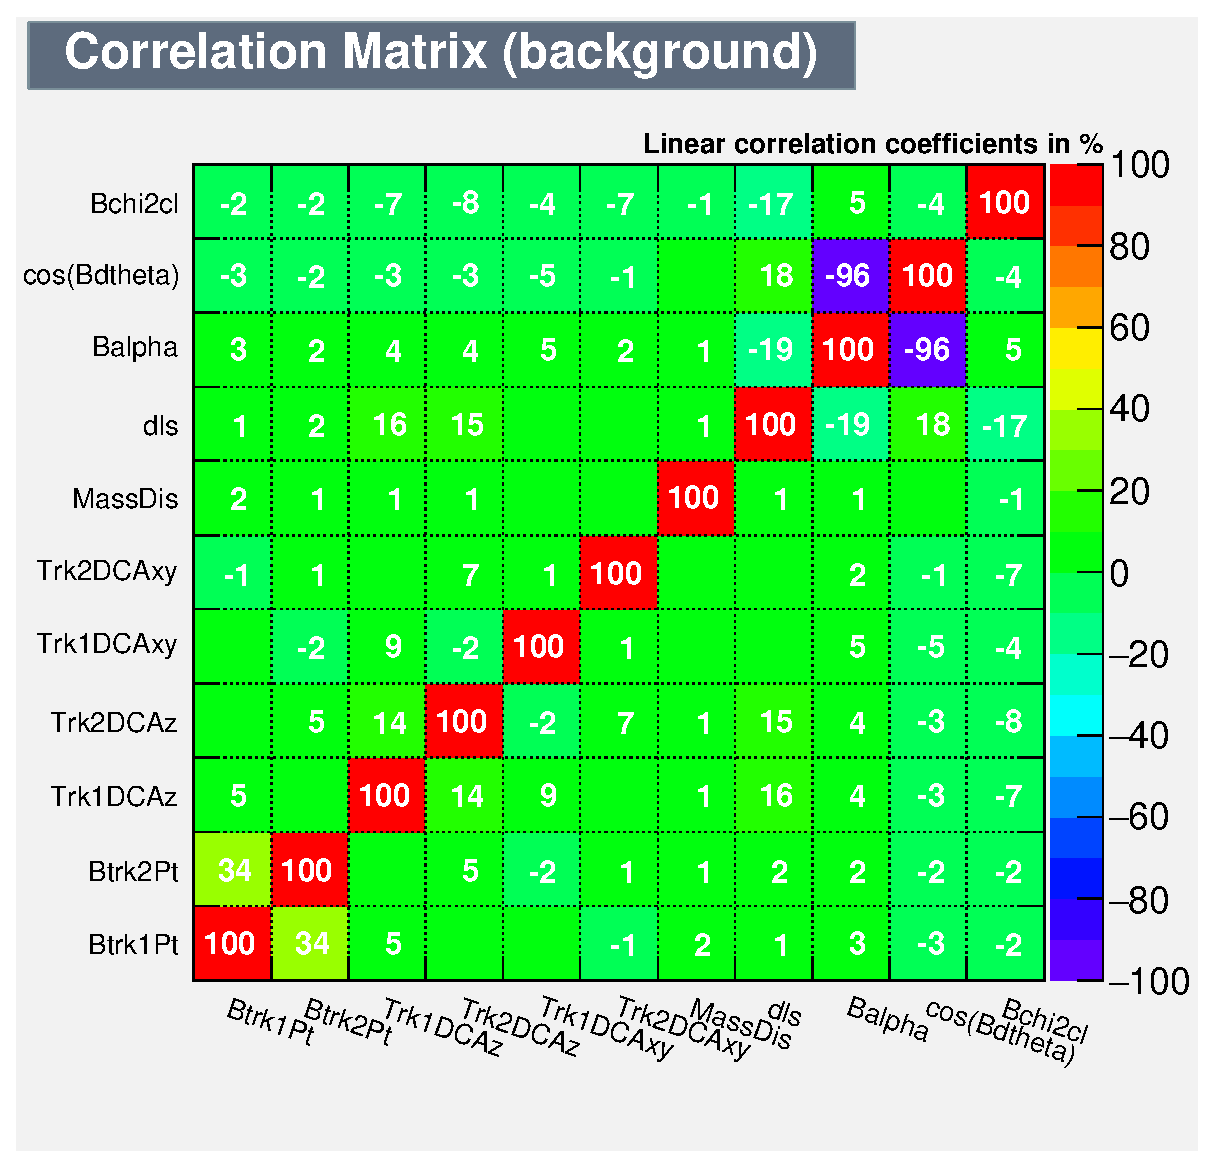
\includegraphics[width= 0.48\textwidth]{Figures/Chapter5/BsCorr_10_15.eps}
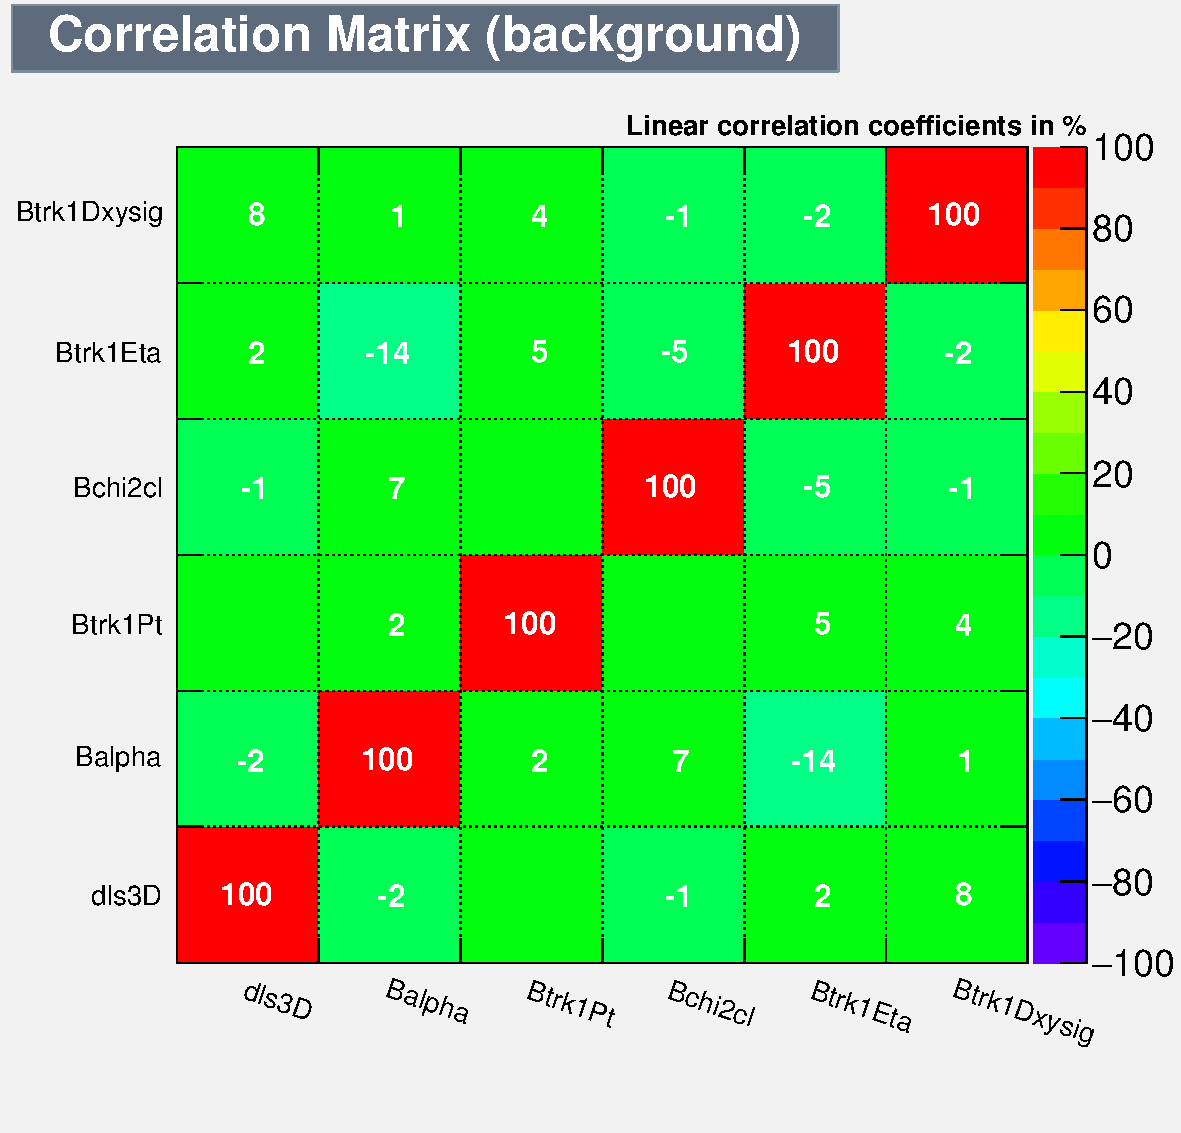
\includegraphics[width= 0.48\textwidth]{Figures/Chapter5/BPCorr_10_15.pdf}
\caption{The correlation matrices of $B^0_s$ (left) and $B^+$ (right) in data at $10 < p_T < 15$ GeV/c are shown above.}
\label{CorrMatrix}
\end{center}
\end{figure}

We can see that there are no significant correlation among the topological variables except for the opening angle $\alpha$ and the cosine its transverse projection $ \cos\theta$, which is known to be correlated. Therefore, the variable sets we input to the \text{TMVA} training are good.  

Next, we compare the overall performance of the algorithms. Figure \ref{ROCAll} below shows the ROC curves for $B^0_s$ \textit{TMVA} training at 10 $< p_T < $ 15 GeV/c.

\begin{figure}[h]
\begin{center}
%\includegraphics[width= 0.80\textwidth]{Figures/Chapter5/BsROC.png}
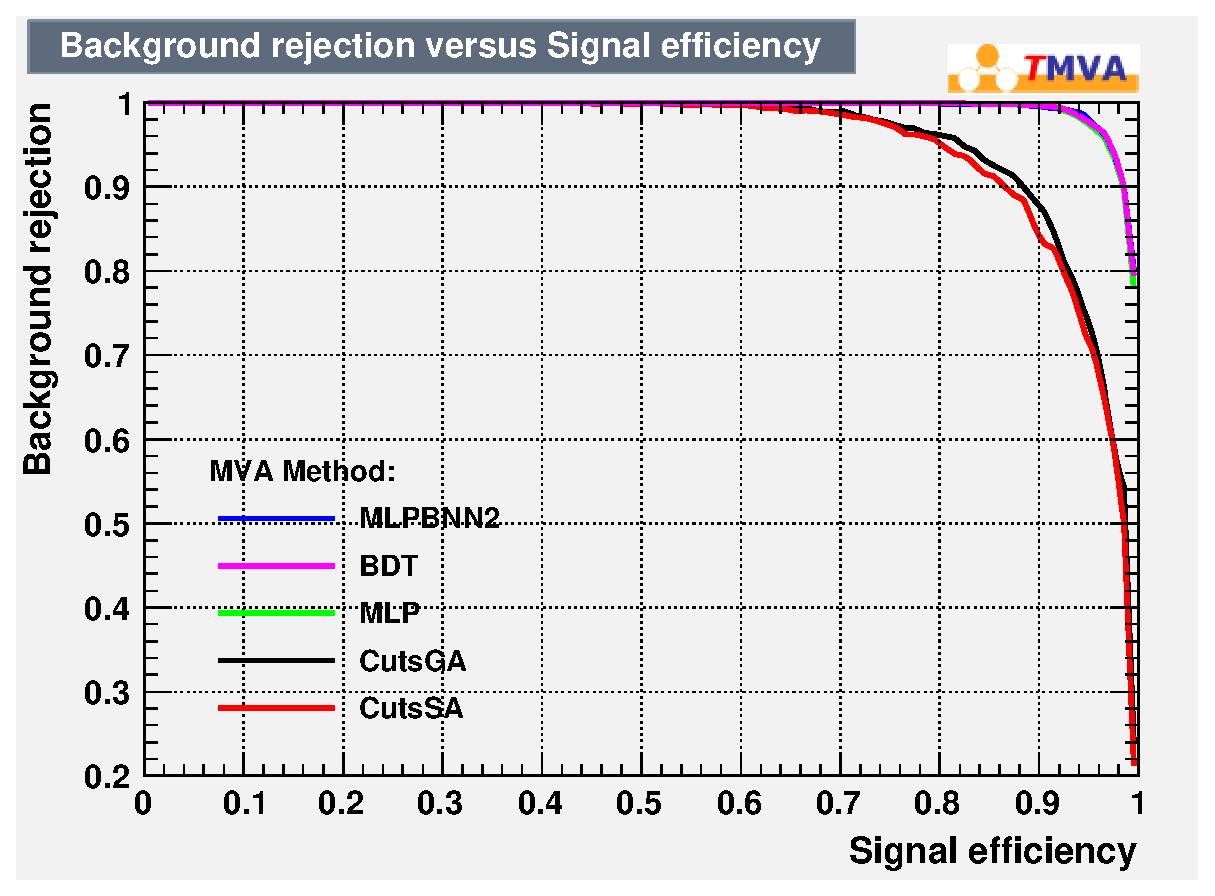
\includegraphics[width= 0.48\textwidth]{Figures/Chapter5/BsROC1015.eps}
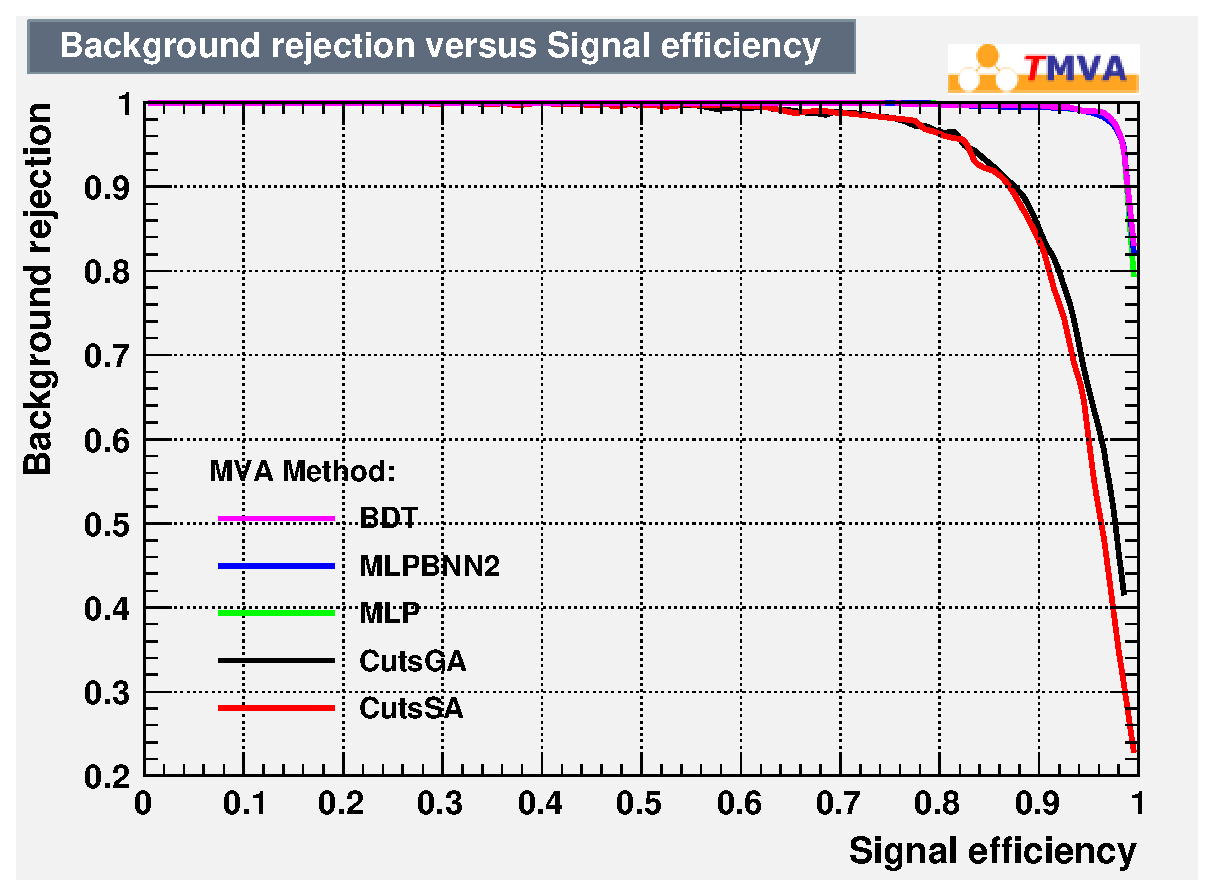
\includegraphics[width= 0.48\textwidth]{Figures/Chapter5/BsROC1520.eps}
\caption{The $B^0_s$ ROC curves of CutsSA, CutsGA, BDT, MLP, and MLPBNN2 algorithms are shown above.}
\label{ROCAll}
\end{center}
\end{figure}

We should note that the number of trees for BDT here is NTree = 2000. From Figure \ref{ROCAll}, we can see that BDT has the best performance compared to other algorithms in the given parameter settings. Basically, for a given background rejection efficiency, the BDT curve has the highest signal efficiency. Or, in order words, the area of BDT ROC curve is the largest among all other algorithms, demonstrating that BDT has the best performance among all other machine learning algorithms. It is closer to the upper right corner, where the best algorithm lies. Therefore, we decide to use the BDT algorithm to look for the optimal selections in all $p_T$ bins in both $B^0_s$ and $B^+$ analysis.


Finally, before, implementing the BDT algorithm to the analysis, we also check the overtraining and make sure that no significant overtraining is observed. Figure \ref{OverTraining} show the overtraining test for both $B^0_s$ and $B^+$ BDT at 10 $< p_T < $ 15 GeV/c. 


\begin{figure}[h]
\begin{center}
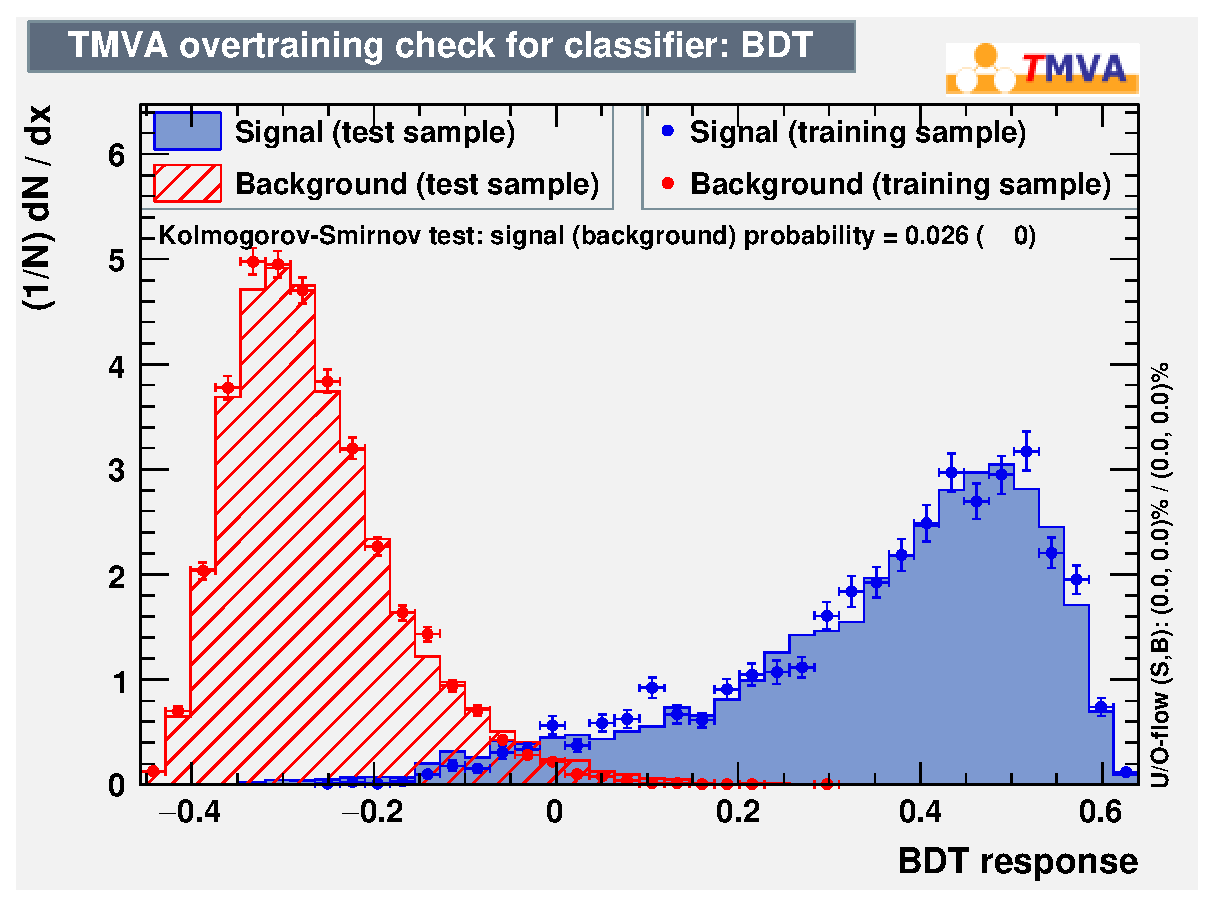
\includegraphics[width= 0.48\textwidth]{Figures/Chapter5/BsOT.eps}
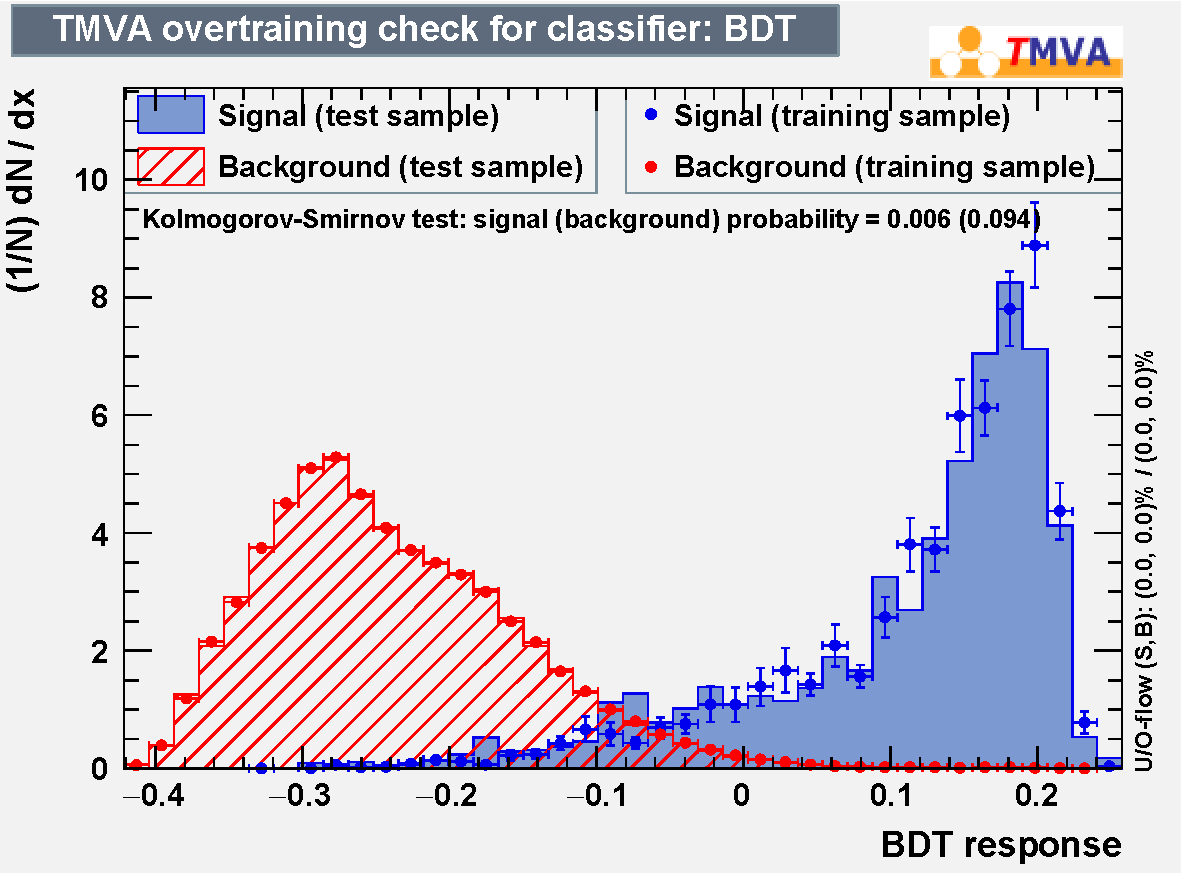
\includegraphics[width= 0.48\textwidth]{Figures/Chapter5/BPOT.pdf}
\caption{The Kolmogorov-Smirnov overtraining tests on the signal (blue) and background (red) in $B^0_s$ (left) and $B^+$ (right) at $10 < p_T < 15$GeV/c are shown on the right. It looks like they both pass the tests.}
\label{OverTraining}
\end{center}
\end{figure}

According to Figure \ref{OverTraining}, neither signal nor background of $B^0_s$ and $B^+$ BDT is vanishing. Hence, no significant overtraining is observed. The BDT training is valid to use in the $B^0_s$ and $B^+$ analysis.


\subsection{Working Point Determination}

Now with the BDT training results, next step is to choose the BDT selection that can give us the best analysis results. We decide to use the statistical significance, which is as follows

\begin{equation}
Sig = \frac{S}{\sqrt{S+B}}
\end{equation}

as the figure of merit. We estimate $S$ and $B$ for a set of BDT cuts and choose the BDT scores that return to the maximum statistical significance in each $p_T$ bin. We can directly estimate the background $B$ according to the data sideband region width scaled to the signal region band width

\begin{equation}
B = \frac{w_{S}}{w_{B}} N_{B} \epsilon_{B}
\end{equation}

To determine the signal $S$, we do not directly look at the data. Instead, we use FONLL cross section \cite{FONLLCal} shown in \ref{FONLL} and the MC to determine the signal $S$ as follows

\begin{equation}
S = 2 R_{AA}^{2015Ref} L \sigma_{FONLL}^{pp\rightarrow b\bar b} \epsilon_{pre} \epsilon_{S} f(b\rightarrow B) BR
\end{equation}

We know that since $B^+$ is more abundantly produced with large reconstructed efficiency since it has only one kaon track compared to $B^0_s$. Therefore, the $B^0_s$ signal statistics is more limited. Table \ref{BsSBCal} summarizes our calculations of $B^0_s$ $S$, $B$, and $S/B$ after the event, track, and muon pre-selections.  


\begin{table}[h]
\begin{center}
\caption{The summary table signal and background estimation of $B^0_s$ in each $p_T$ and centrality bin in the analysis.}
\vspace{1em}
\label{BsSBCal}
  \begin{tabular}{ |c|c|c|c|c|}
    \hline 
Centrality (\%) & $B^0_s$ $p_T$ (GeV/c) & Signal ($S$) & Background ($B$) & $S/B$ Ratio \\
     \hline
0 -- 90 & 7 -- 10 & 12 & 24234 & 0.000495  \\
0 -- 90 & 10 -- 15 & 47 &14230  & 0.00330 \\
0 -- 90 & 15 -- 20 &24 & 2457 & 0.00977 \\
0 -- 90 & 20 -- 50 & 25 & 698 & 0.0358 \\
0 -- 30 & 10 -- 50 & 64 &  16697 & 0.00383 \\
30 -- 90 & 10 -- 50 &32 & 688 & 0.0465 \\
0 -- 90 & 10 -- 50 & 96 &17385  &  0.00552\\
     \hline
    \hline
\end{tabular}
\end{center}
\end{table}



Now, we scan through a series of BDT values from -1 to 1 and compute their corresponding statistical significance. Figure \ref{WorkingPoint} shows the statistical significance as a function of BDT for $B^0_s$ and $B^+$ at $10 < p_T <  15$ GeV/c

\begin{figure}[h]
\begin{center}
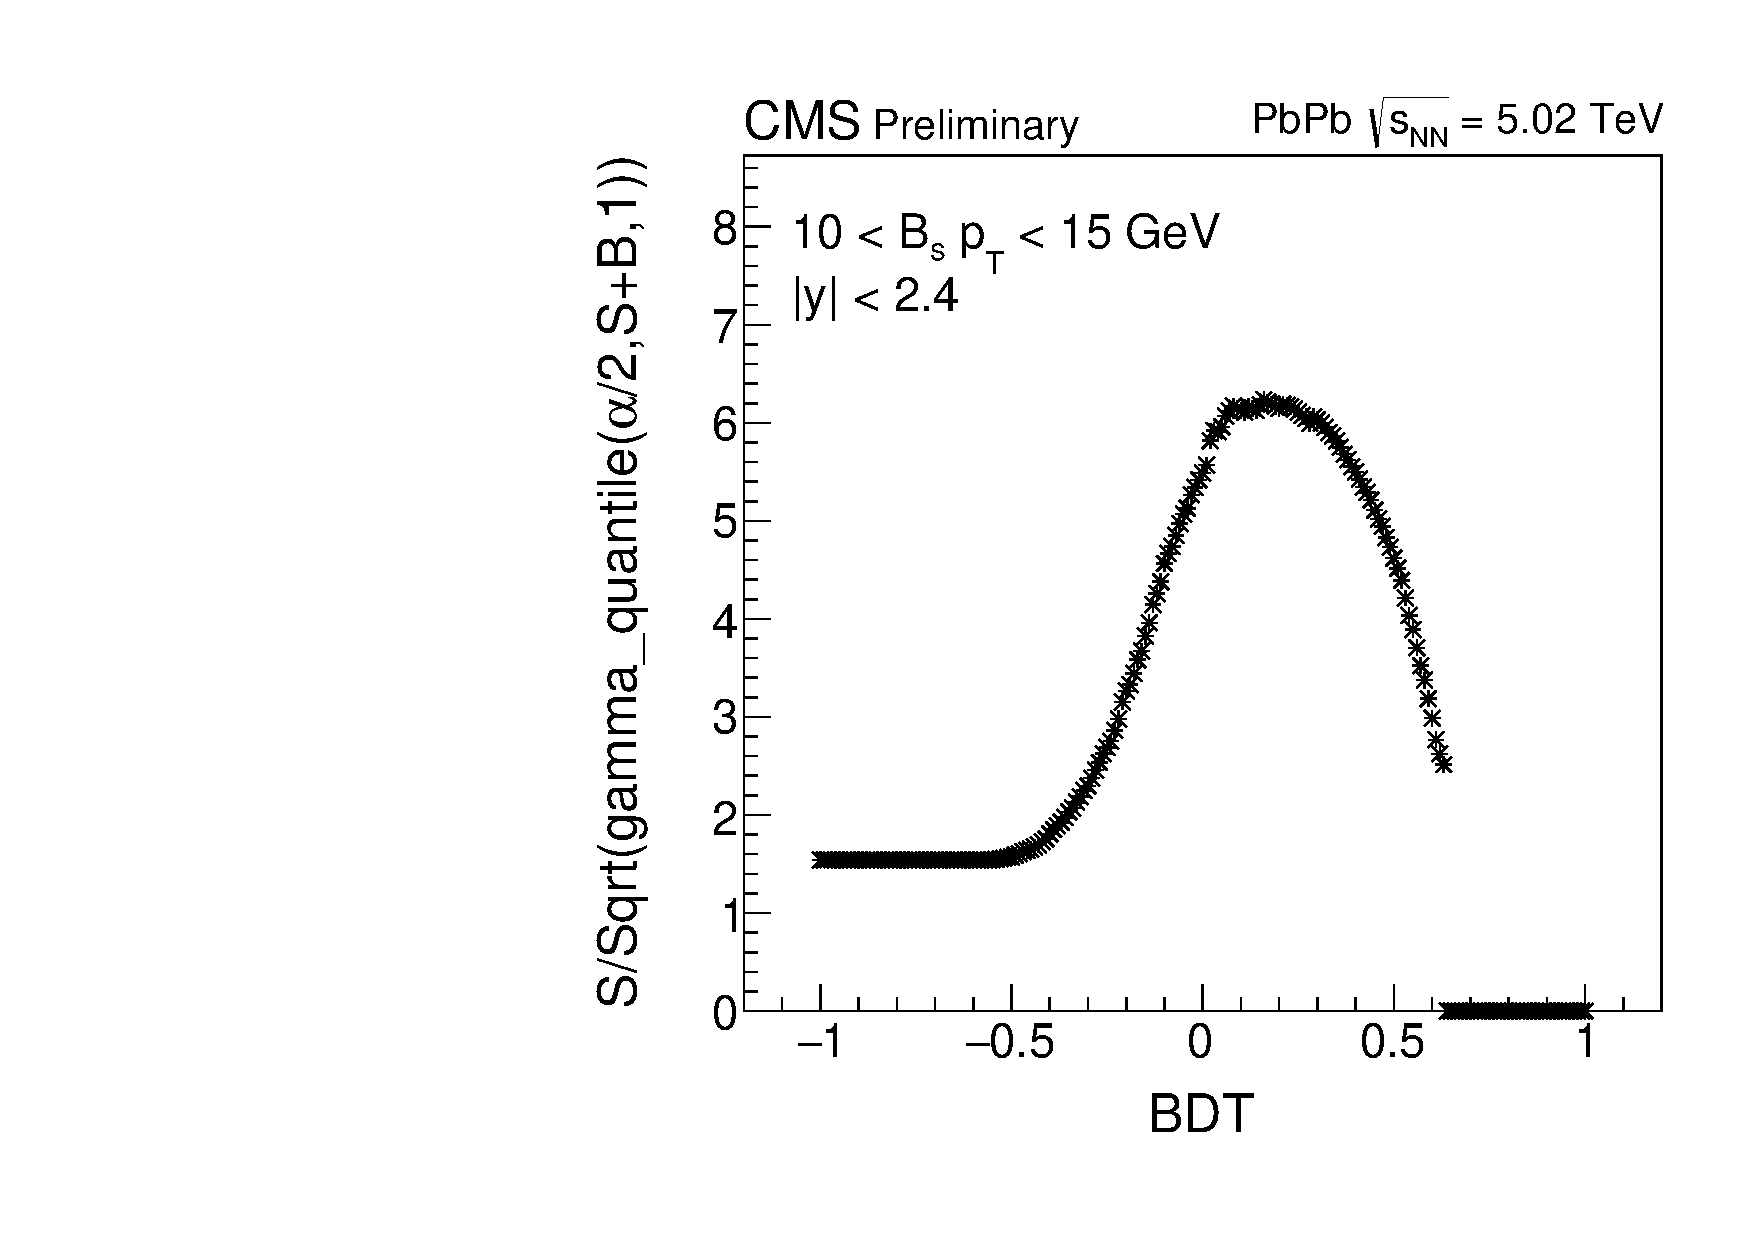
\includegraphics[width= 0.40\textwidth]{Figures/Chapter5/BsSig_10_15.pdf}
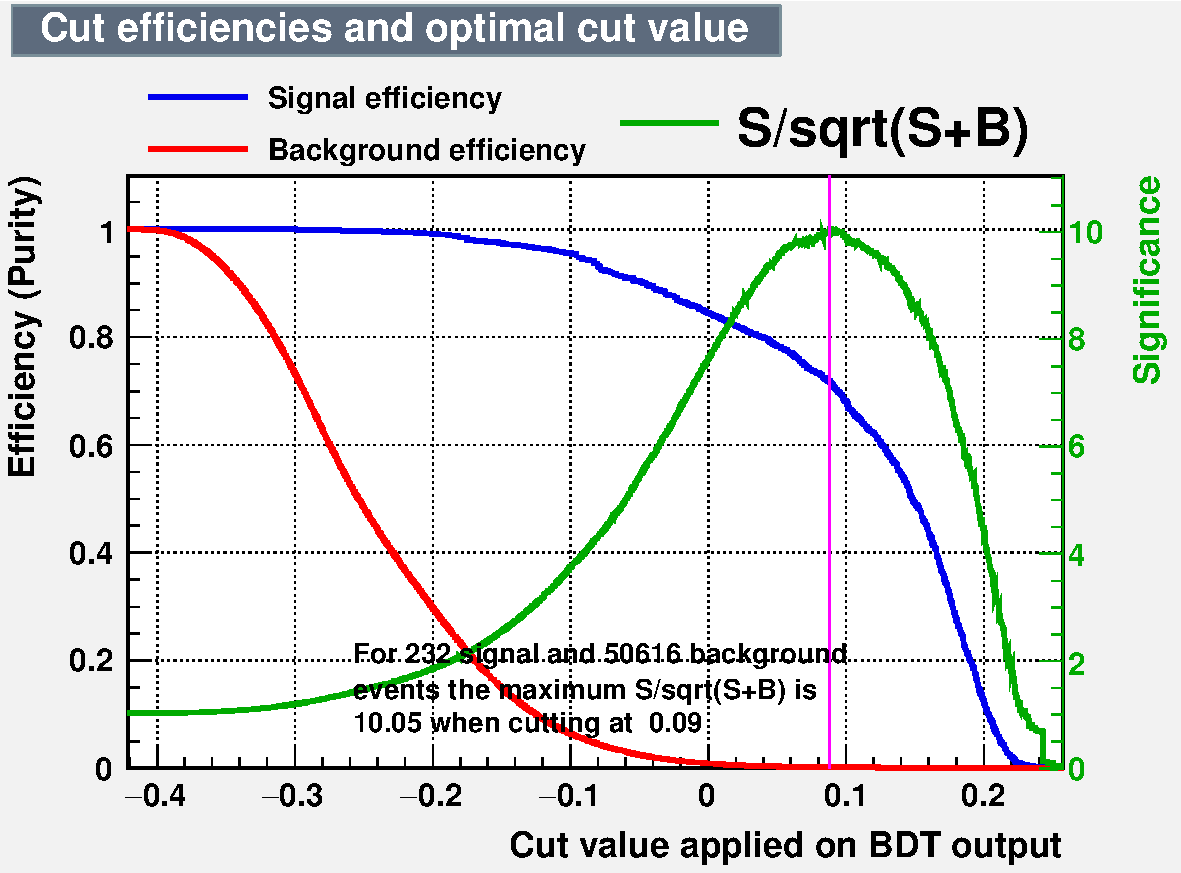
\includegraphics[width= 0.53\textwidth]{Figures/Chapter5/BPSig_10_15.pdf}
\caption{The significance: $Sig = \frac{S}{\sqrt{S+B}}$ as a function of BDT in $B^0_s$ at $10 < p_T <  15$ GeV/c are shown above. We can see that $B^0_s$ BDT peaks near 0.32 while $B^+$ peaks near 0.09.}
\label{WorkingPoint}
\end{center}
\end{figure}

For $B^0_s$  Our optimal selection returns us with an S = 38 and B = 5, which has a remarkable background-to-signal rejection of more than $10^3 : 1$.



Table \ref{BsSig} and \ref{BPSig} document the optimal BDT selections maximizing the statistical significance in each $p_T$ bin for $B^0_s$ and $B^+$ respectfully.

\begin{table}[h]
\begin{center}
\caption{The summary of optimal BDT selection maximizing the $B^0_s$ statistical significance.}
\vspace{1em}
\label{BsSig}
  \begin{tabular}{ |c | c| c| c| c|}
    \hline 
$B^0_s$ $p_T$ (GeV/c) & 5 -- 10 & 10 -- 15 & 15 -- 20 &  20 -- 50\\
     \hline
 BDT Cut Values & $>$ 0.32 & 0.29  & 0.35 & 0.33  \\
     \hline
    \hline
\end{tabular}
\end{center}
\end{table}

\begin{table}[h]
\begin{center}
\caption{The comparison of the traditional rectangular selections to MVA for Figure \ref{MVADemo}.}
\vspace{1em}
\label{BPSig}
  \begin{tabular}{ |c | c| c| c| c| c| c| c| c|}
    \hline 
$B^+$ $p_T$ (GeV/c) & 5 -- 7 & 7 -- 10 & 10 -- 15 & 15 -- 20 & 20 -- 30 & 30 -- 40 & 40 -- 50 & 50 -- 60\\
     \hline
 BDT Cut Values & $>$ 0.02  & 0.03  & 0.09 & 0.07  & 0.10 & 0.16 & 0.20 & 0.27  \\
     \hline
    \hline
\end{tabular}
\end{center}
\end{table}


\subsection{Optimal Selection Performance}

To check the performance BDT selections, we look at the dimuon and dikaon invariant mass distributions to see if $J/\psi$ and $\phi$ resonance are observed. Figure \ref{mesonpeak} shows the after applying the selections


\begin{figure}[h]
\begin{center}
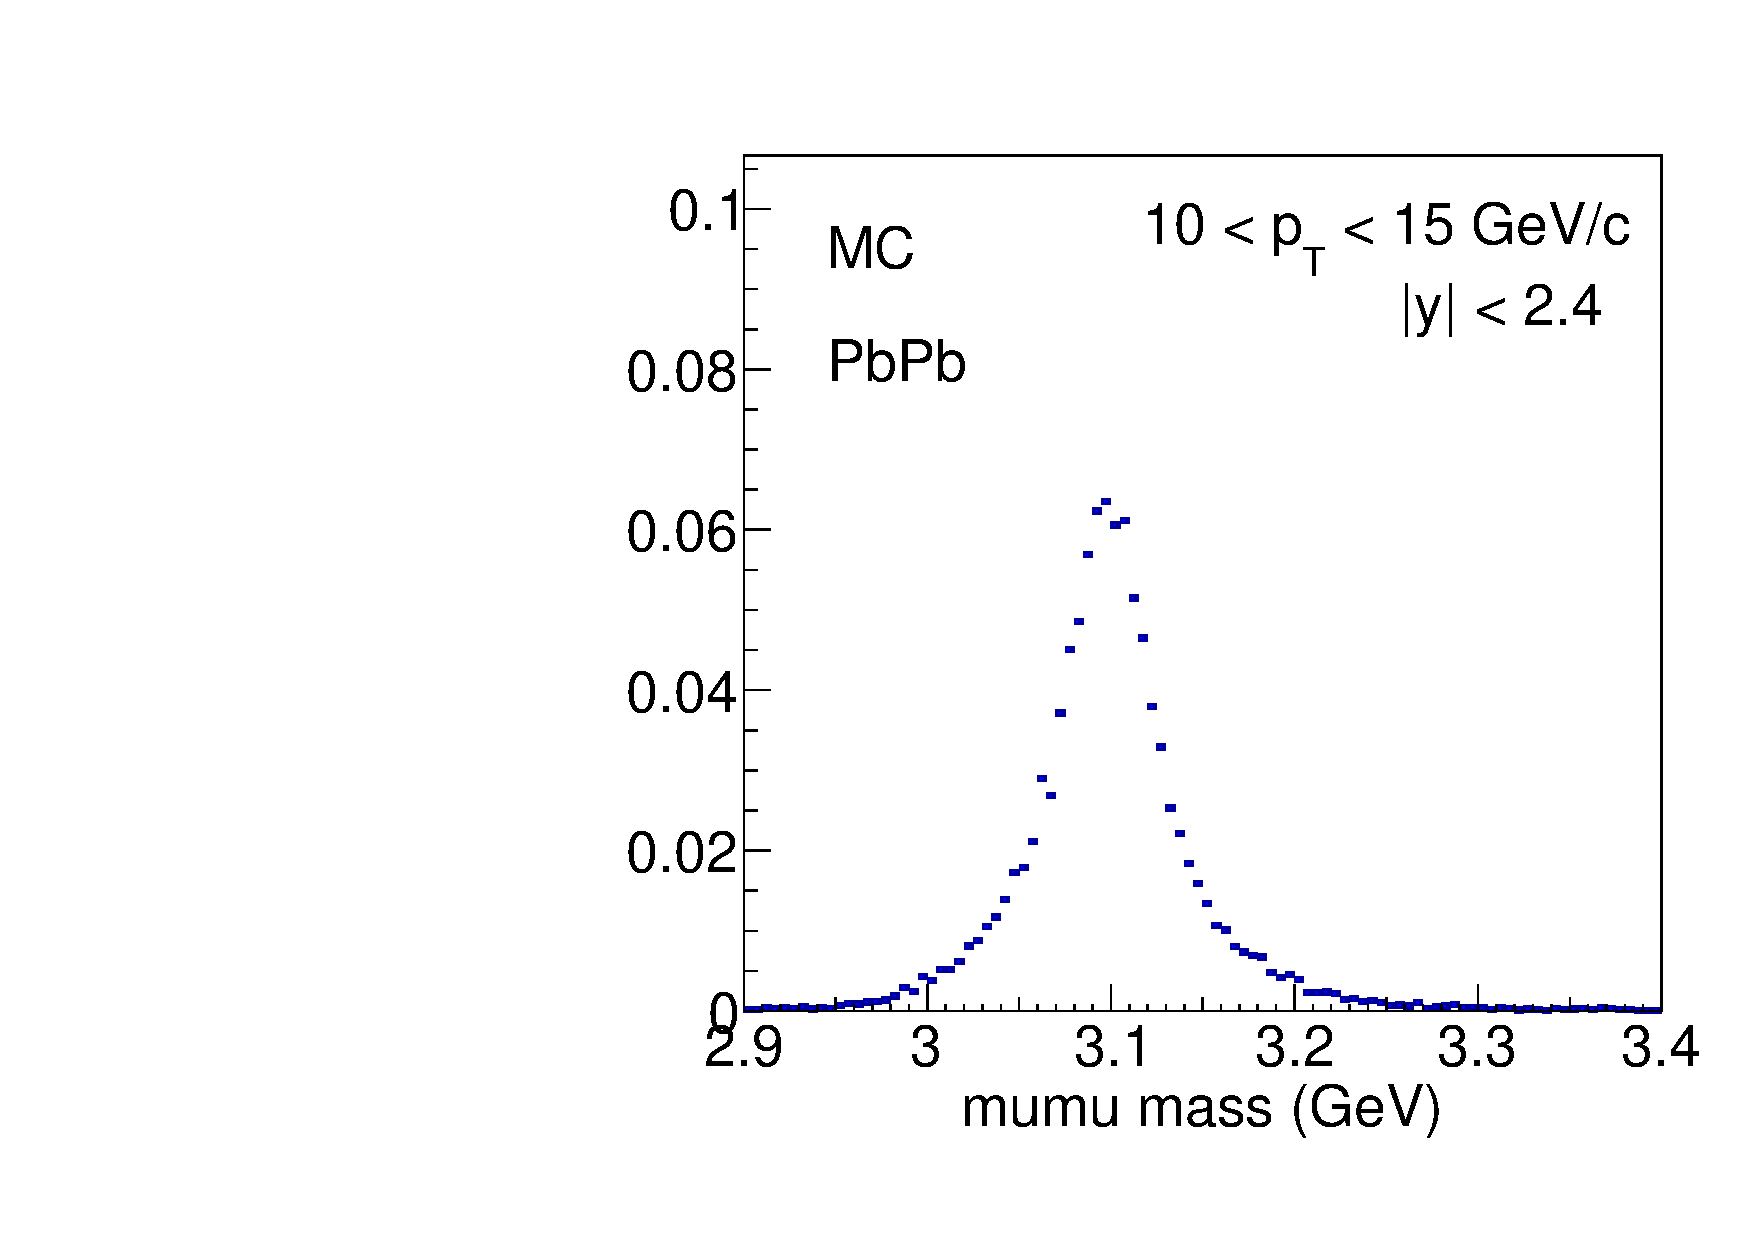
\includegraphics[width=0.42\textwidth]{Figures/Chapter5/mc_PbPb_1_Bmumumass.pdf}
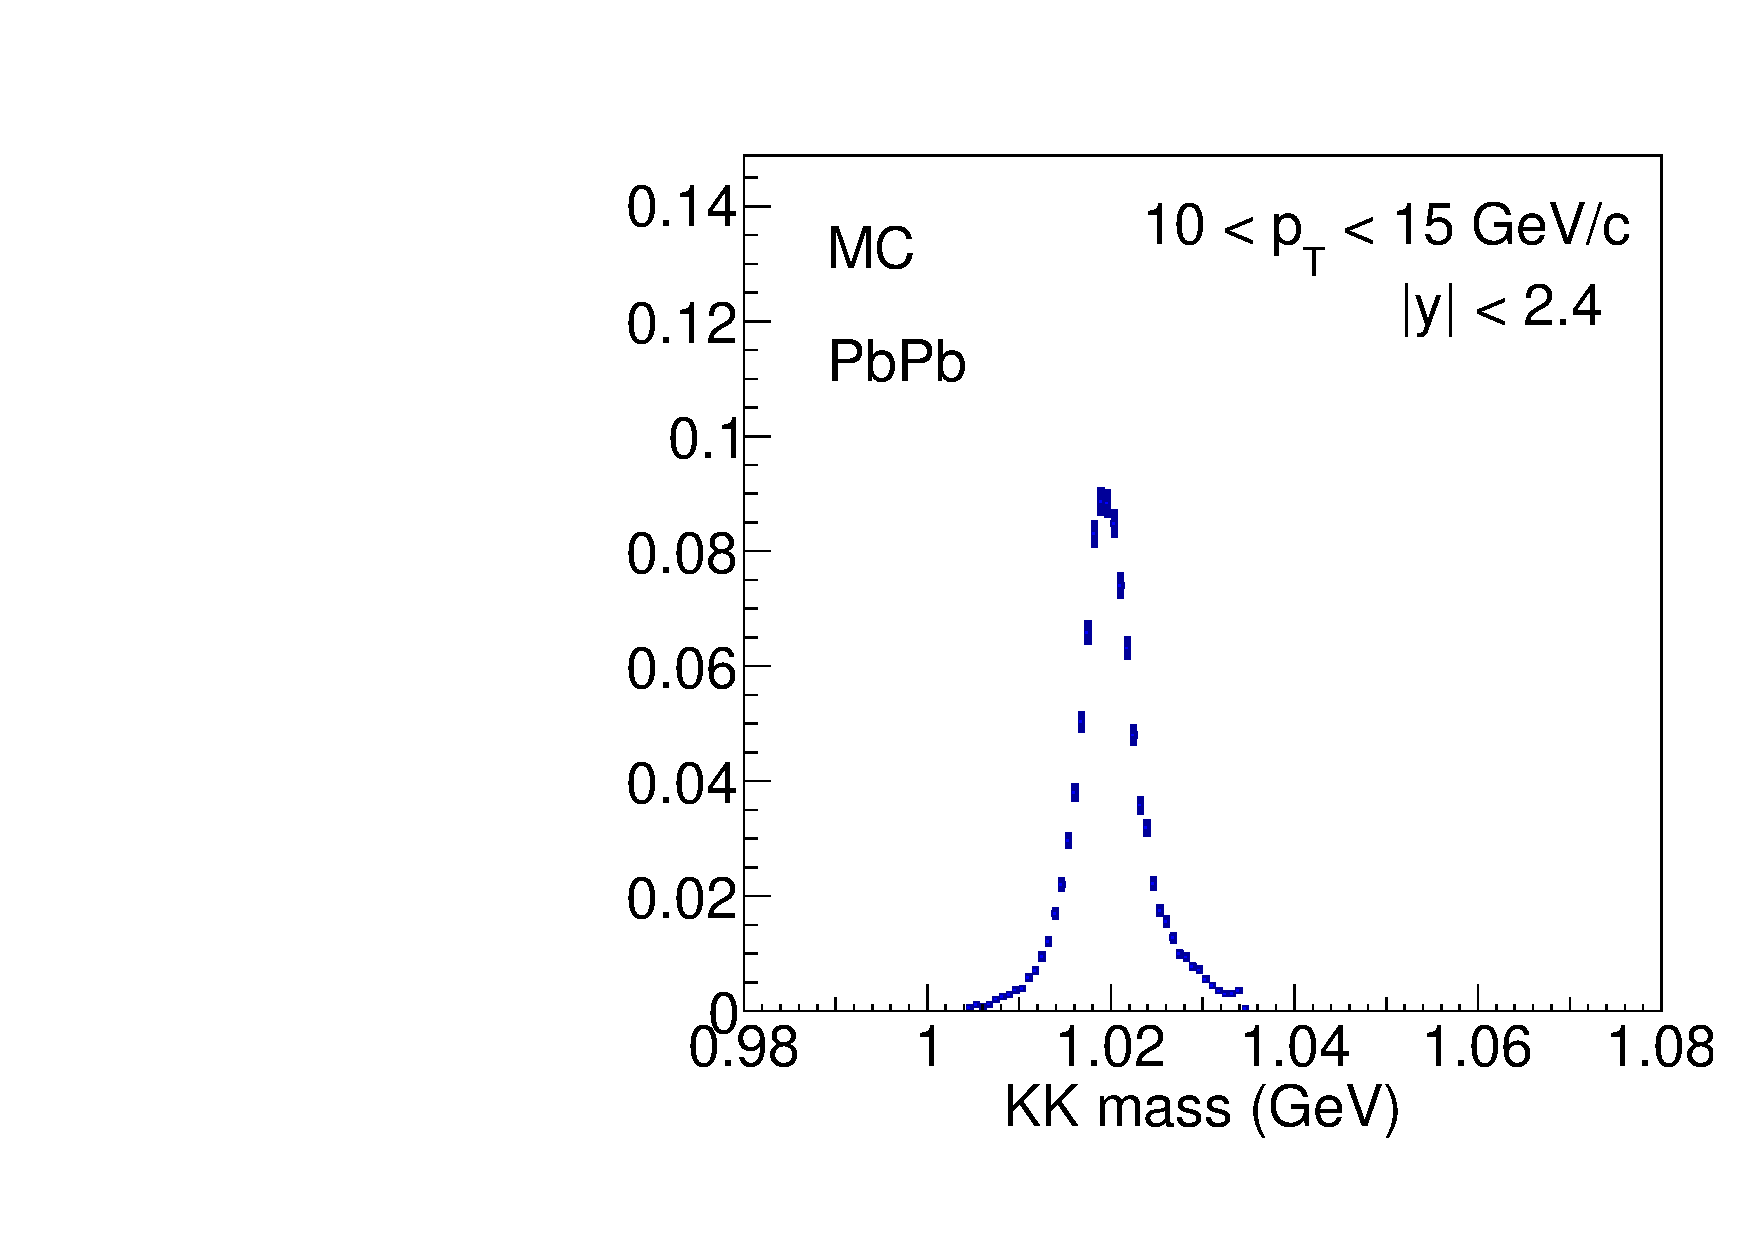
\includegraphics[width=0.42\textwidth]{Figures/Chapter5/mc_PbPb_1_Btktkmass.pdf}
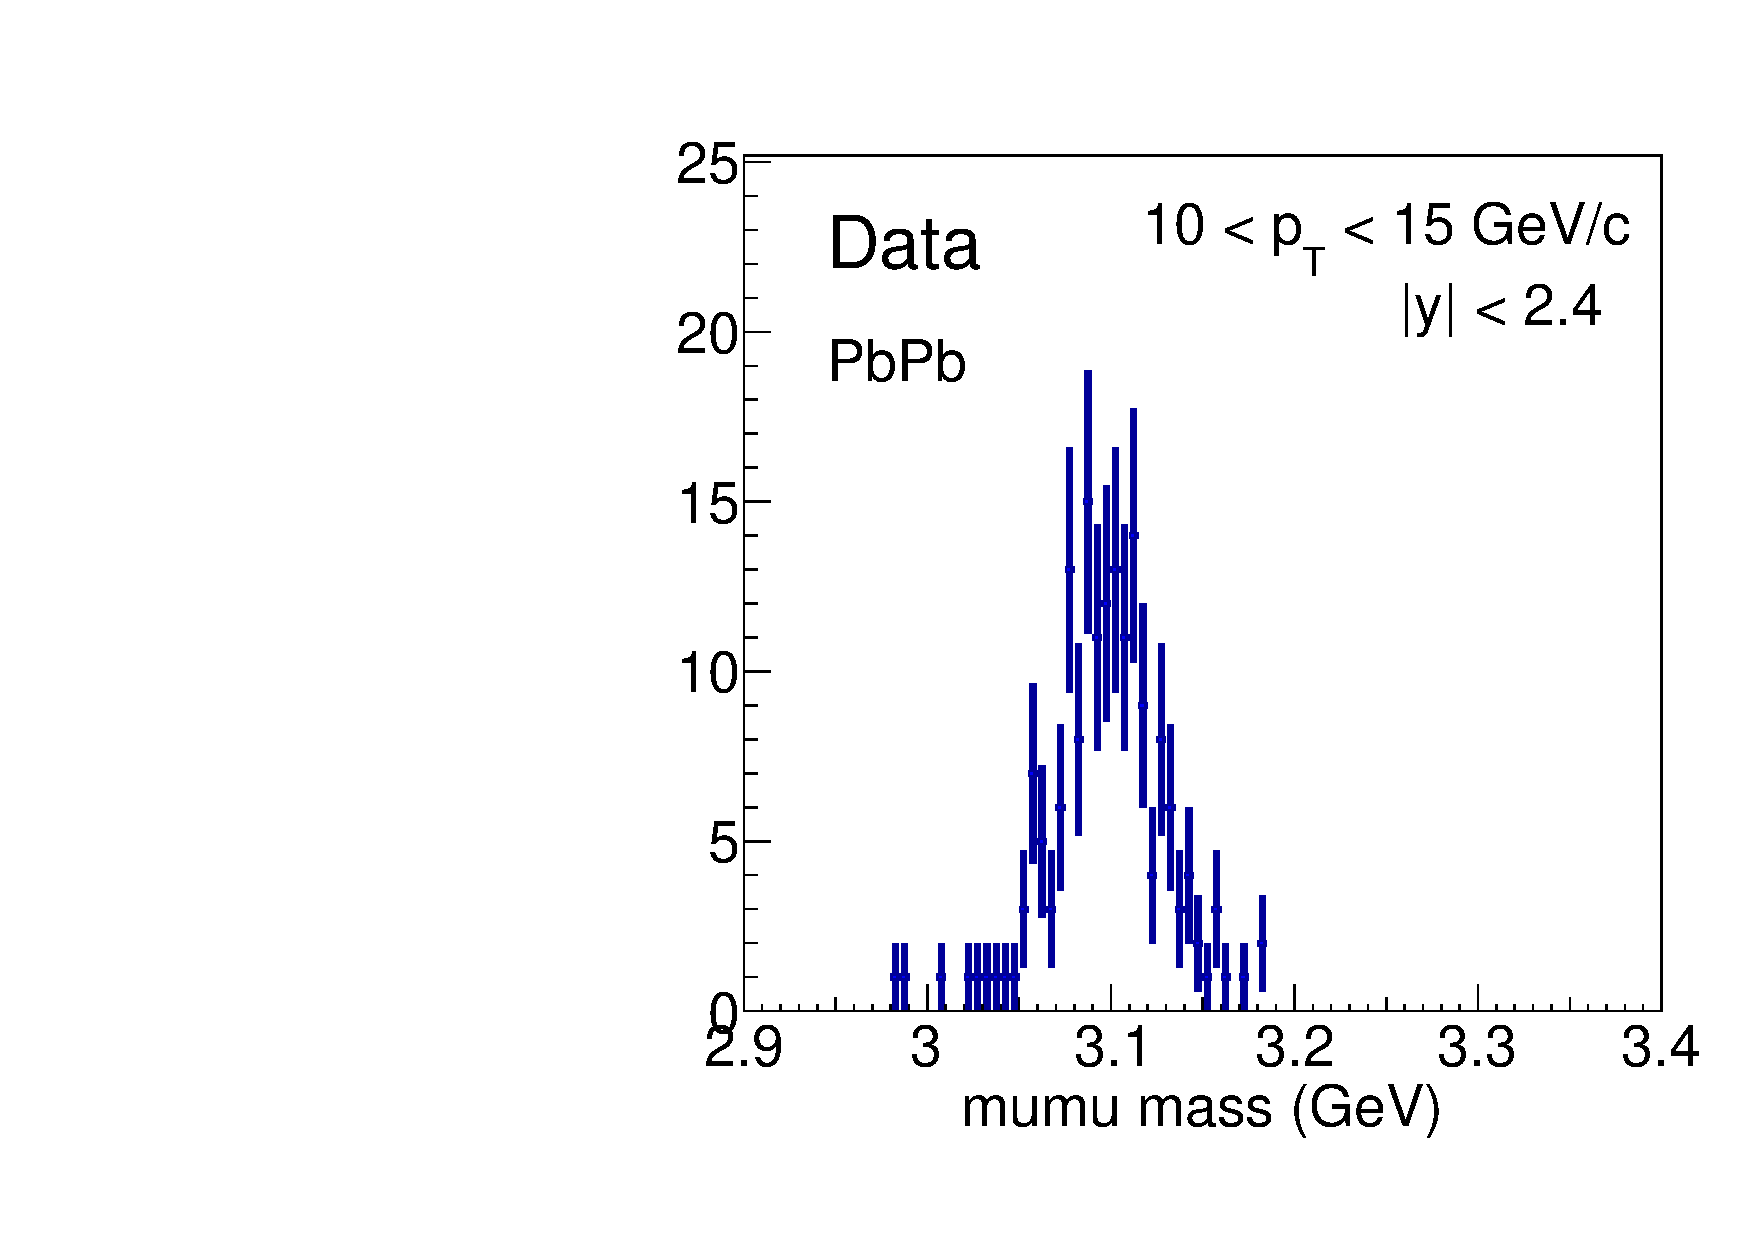
\includegraphics[width=0.42\textwidth]{Figures/Chapter5/data_PbPb_1_Bmumumass.pdf}
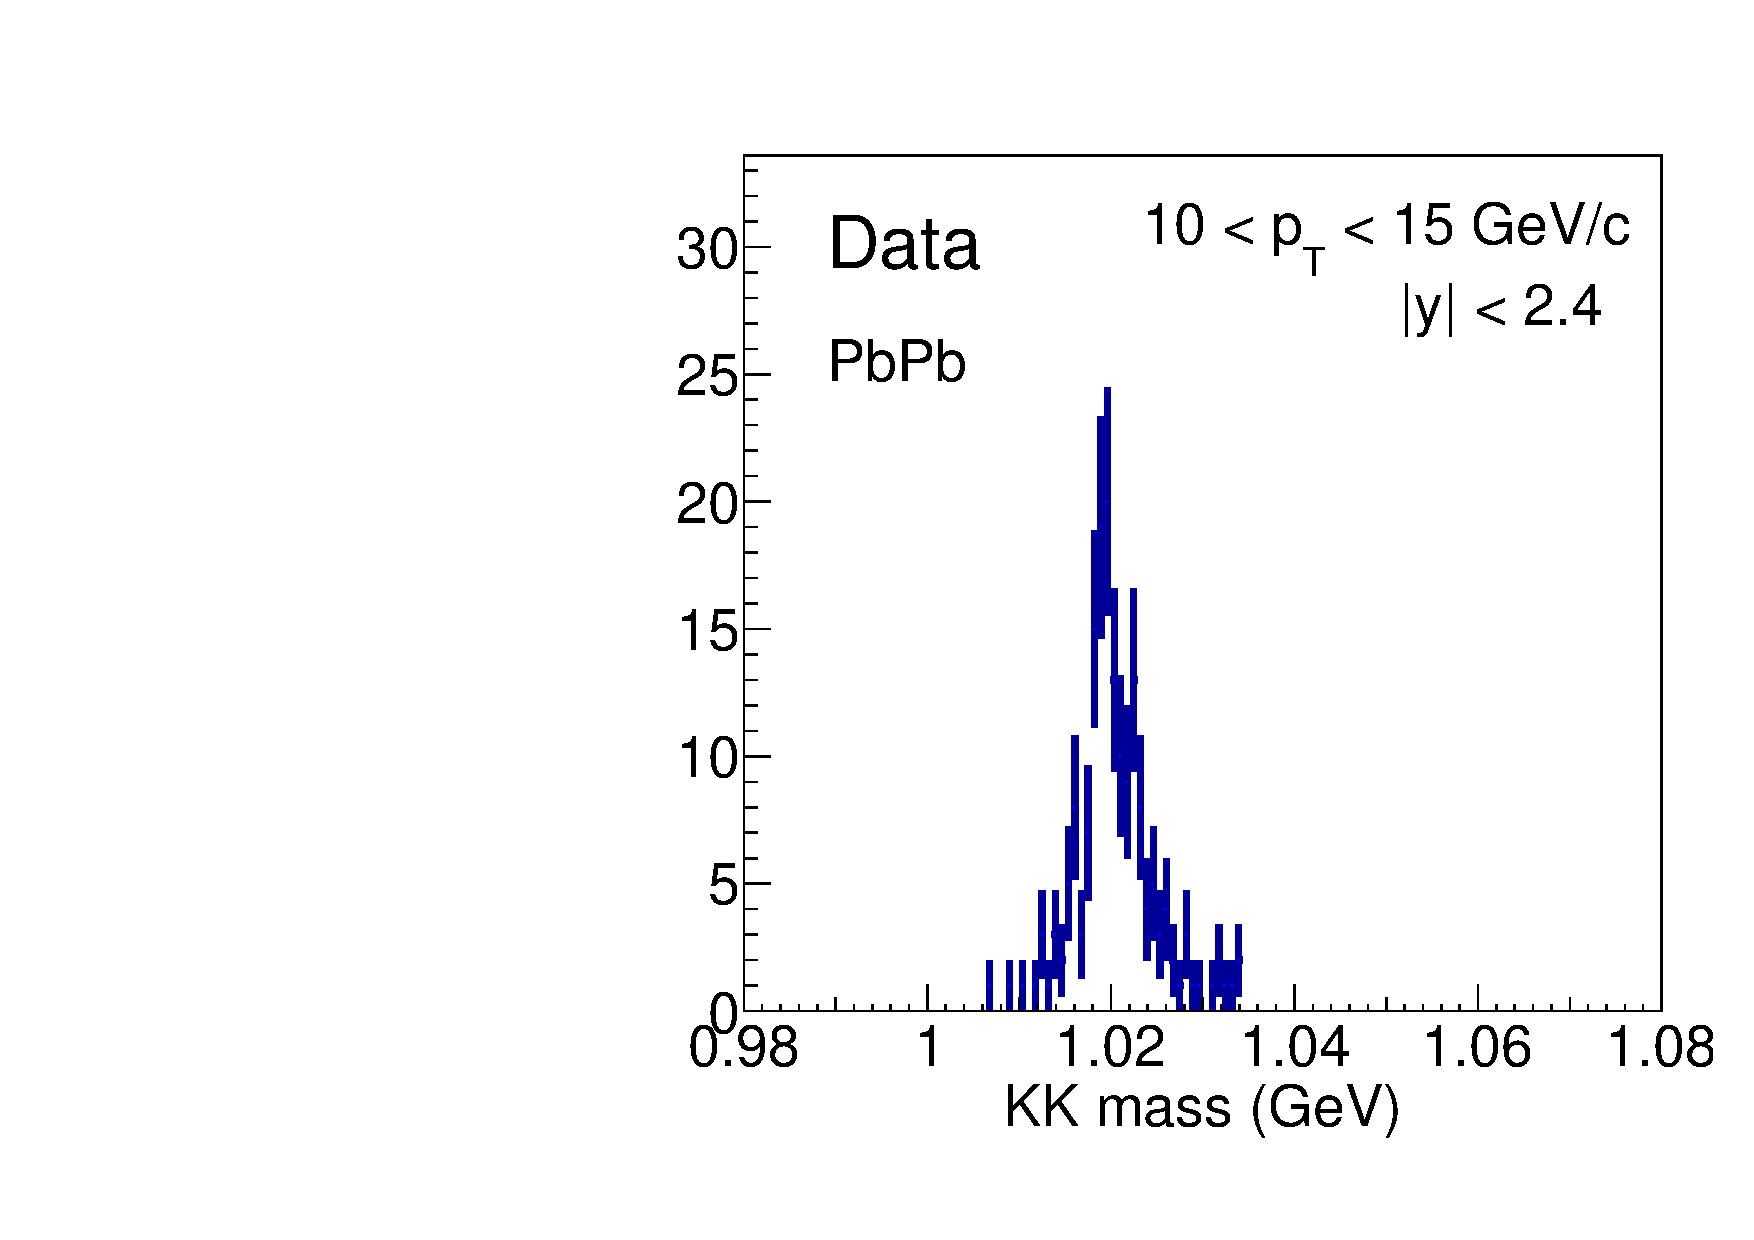
\includegraphics[width=0.42\textwidth]{Figures/Chapter5/data_PbPb_1_Btktkmass.pdf}
\caption{The $J/\psi$ (left) and $\phi$ (right) meson mass distributions after applying BDT > 0 for MC (top) and data (low) in $B^0_s$ analysis are shown above.}
\label{mesonpeak}
\end{center}
\end{figure}

We can see clear $J/\psi$ and $\phi$ peaks after applying the selections in both data and MC, which suggests that our selections are reasonable. Now we can also look at the invariant mass distributions of $B^0_s$ and $B^+$ in Figure \ref{Bpeaks}

\begin{figure}[h]
\begin{center}
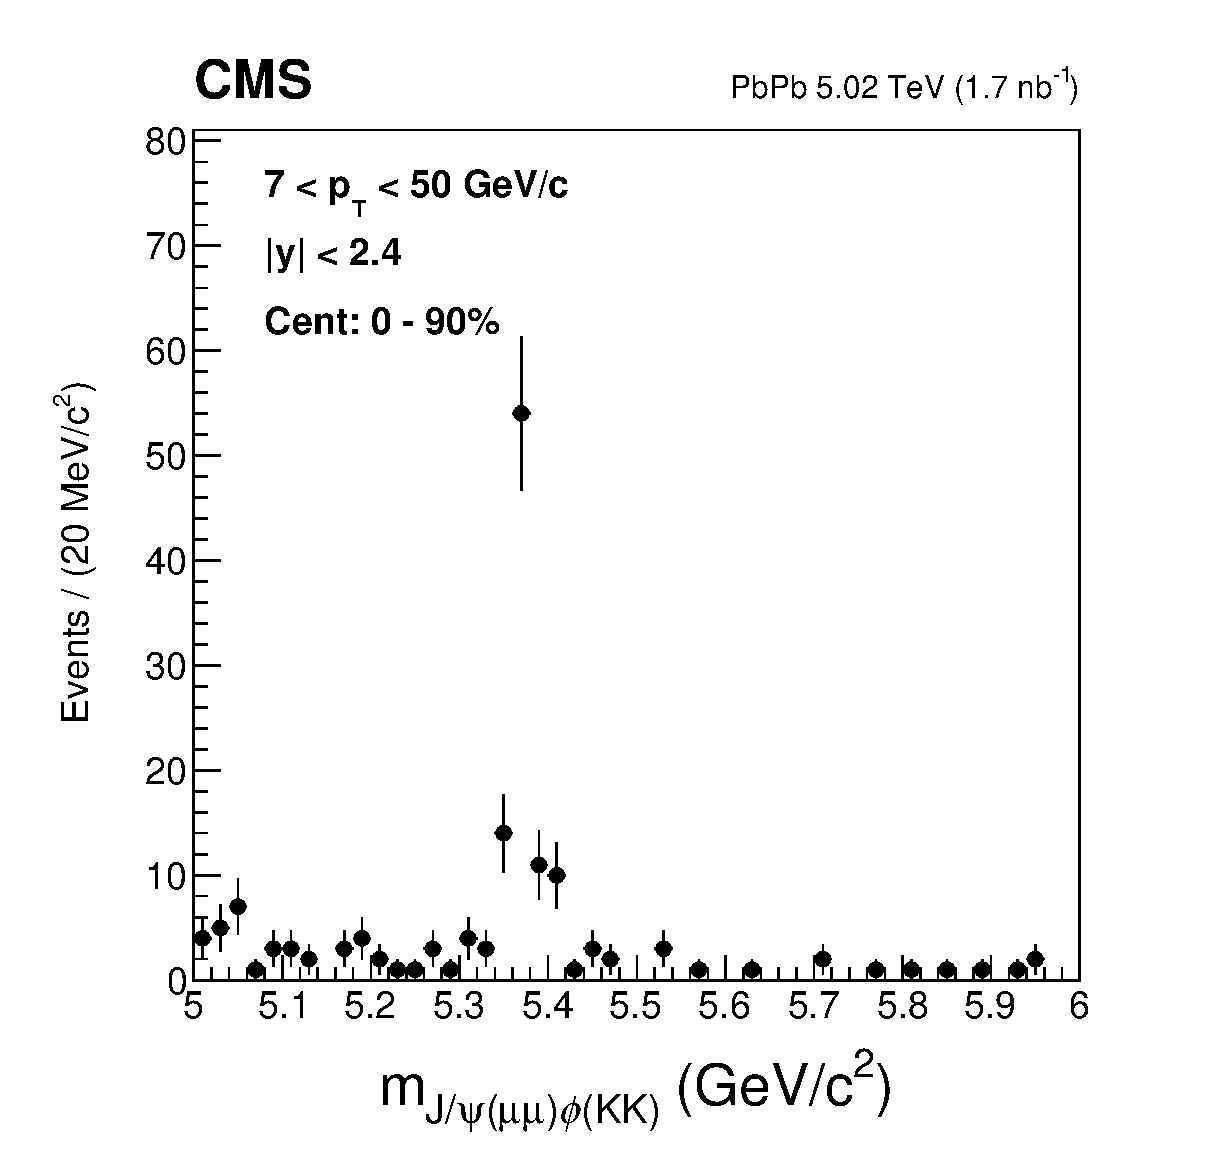
\includegraphics[width=0.42\textwidth]{Figures/Chapter5/BsMassBDTCut.eps}
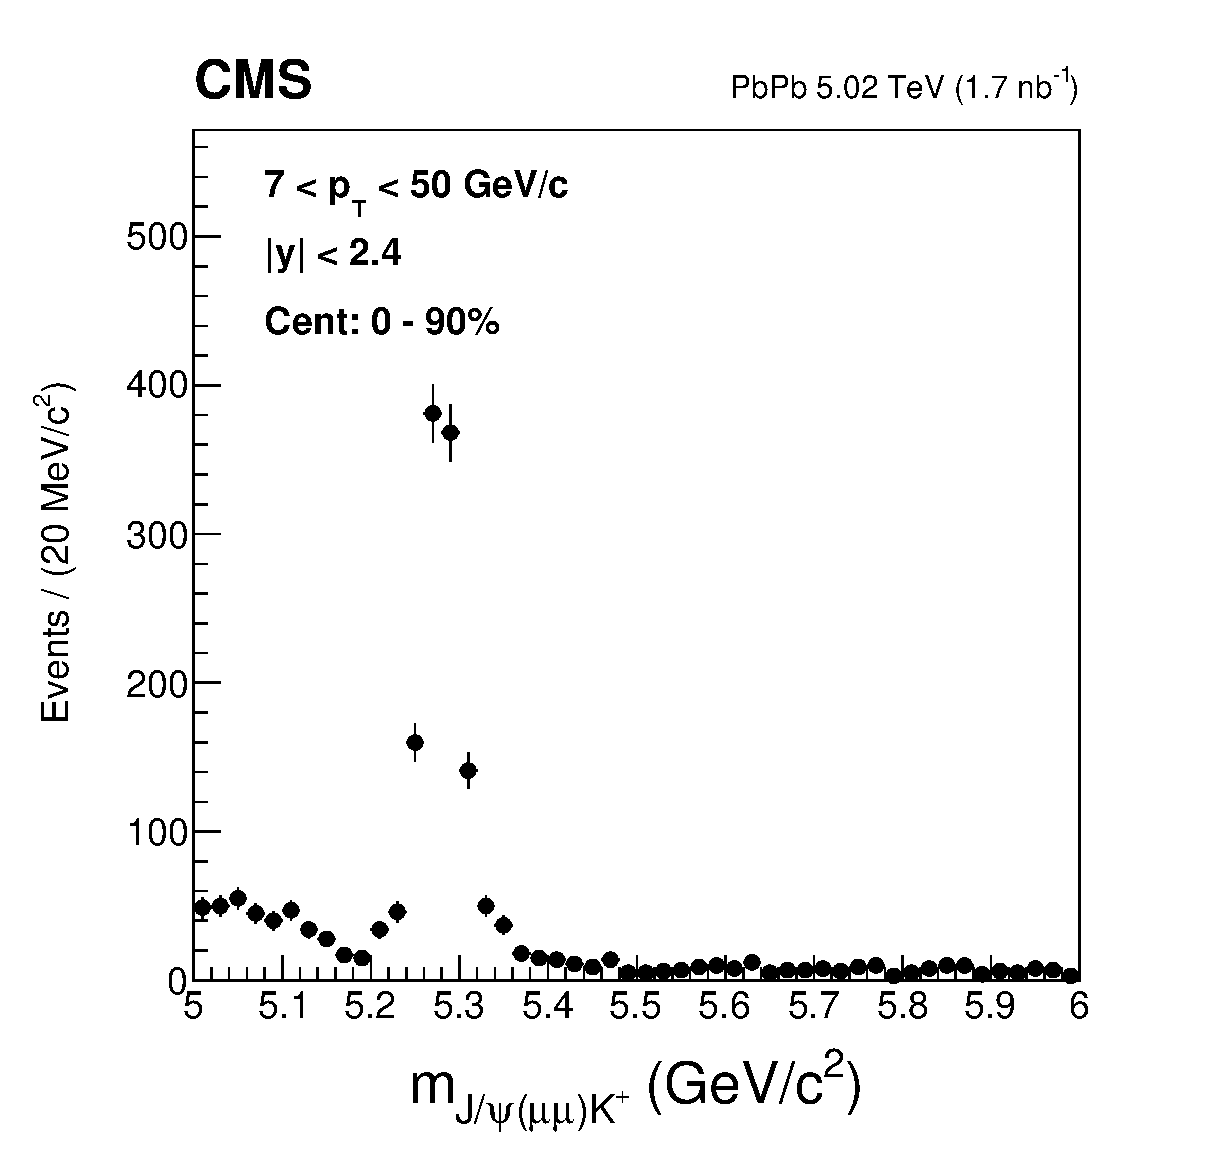
\includegraphics[width=0.42\textwidth]{Figures/Chapter5/BPMassBDTCut.eps}
\caption{The $B^0_s$ (left) and $B^+$ (right) invariant mass distributions after applying optimal BDT selections from $10 < p_T < 50$ GeV/c in data are shown above.}
\label{Bpeaks}
\end{center}
\end{figure}

Again, we can see very clear signals after the optimal BDT selections in both $B^0_s$ and $B^+$ invariant mass distributions. Now we are ready to study its background and signal before extracting the raw yield for B-meson cross section measurement.

\section{Background Studies} 

\subsection{Overview}

The production of $J/\psi$ mesons occurs in three ways. The prompt $J/\psi$ produced directly in the proton-proton collision or indirectly via the decay of heavier charmonium states, and non-prompt $J/\psi$ from the decay of a b hadron. Non-prompt $J/\psi$ lead to a measurement of the b-hadron cross section. According to PDG, so far physicists have observed thousands of known decay modes of b hadrons \cite{AlphaTheoEx}. Without hadronic PID, we can envision that potential background feed-down sources are coming from other B-meson decays in the B-meson invariant mass spectrum. For instance, the decay of $B^0 \rightarrow J/\psi K^{*0} (892) \rightarrow \mu^+ \mu^- K\pi$ could contribute to the $B^0_s \rightarrow J/\psi \phi \rightarrow \mu^+ \mu^- K^+ K^-$ due to misidentification of $\pi$ to $K$. We call such background as ``non-prompt (NP) background'', to distinguish them from the combinatorial background due to random combinations of decay daughters when reconstructing B mesons. NP background generally forms a peaking structure in the region of interests. A dedicated inclusive NP $J/\psi$ from b hadron decay MC is simulated to determine the NP background component near our B-meson invariant mass region. We then classify each reconstructed B-meson candidate by their GEN-level particle, e.g. whether it is coming from a $B^{0}$, $B^{+}$, or other decays that fall into the B-meson reconstruction workflow, in order to measure their individual contribution to the peaking structure.


\subsection{Individual Channel NP Background Studies} 


\label{sec:individual_channels}
Many small contributions form peaking background structure. We can not identify each of them individually but most of the contributed ones are determined.
Below is a list of example processes that compose the majority of the peaking background:

\begin{itemize}
\item {Case 1: $ X \rightarrow J/\psi  \pi^{-}  K^{+}$, here pion is mis-identified as kaon}
\item {Case 2: $ B_{s}^{0} \rightarrow J/\psi  K^+ K^- $, in which both Kaons are not coming from the decay of an intermediate $\phi$ meson resonance.}
\item {Case 3: $ B^{+} \rightarrow J/\psi  K^{+}$, (added extra $K^-$)} 
\item {Case 4: $ X \rightarrow J/\psi  \pi^{+} \pi^{-}$, pions mis-identified as Kaons. }
\item {Case 5: $ B_{s}^{0} \rightarrow J/\psi K^{+} K^{-} X $ }
\item {Case 6: $ B_{s}^{0} \rightarrow J/\psi \phi \pi \pi $}
\item {Case 7: $B^0 \rightarrow J/\psi  K^{*0} $}
%\item {8 th case $ \chi_{1c} \rightarrow J/\psi \gamma$ }
%\item {9 th case $ \psi_{2s} \rightarrow J/\psi  X $}
\end{itemize}

Figure \ref{BsNPbkgd} shows the contribution of the determined channels with respect to the total background after applying optimal cuts for PbPb for 10 $< p_T <$ 15 GeV/c, 10 $< p_T <$ 20 GeV/c, 20 $< p_T <$ 50 GeV/c, as well as the inclusive 10 $< p_T <$ 50 GeV/c. The peak at the $B_{s}^{0}$ signal region has been investigated and found out that mostly contributed channels are $B^0 \rightarrow J/\psi  K^{*0} (892)$ in grey color and $ B_{s}^{0} \rightarrow J/\psi  K^{+} K^{-}$ in black color. 


\begin{figure}[ht!]
\centering
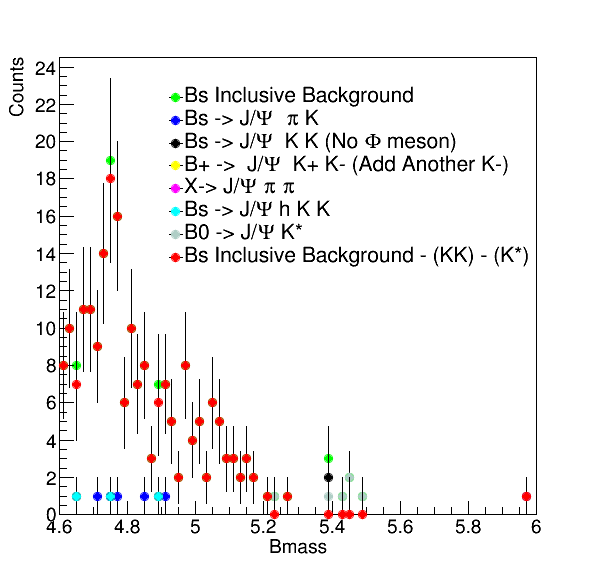
\includegraphics[width=0.45\linewidth]{Figures/Chapter5/NPBackgroundONLY_0.png}
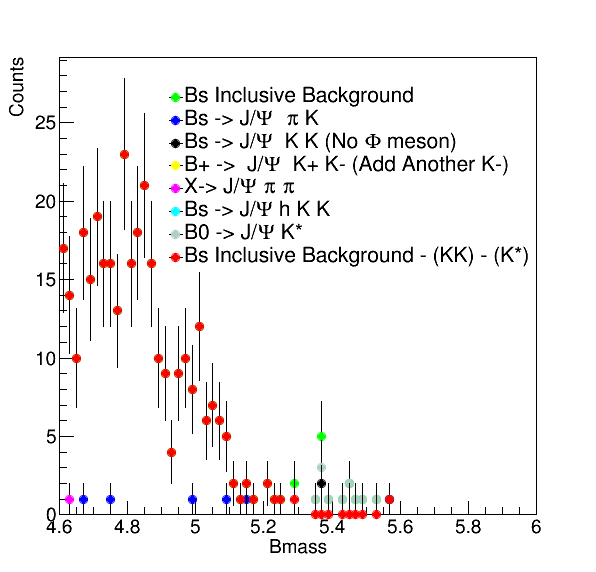
\includegraphics[width=0.45\linewidth]{Figures/Chapter5/NPBackgroundONLY_1.png}
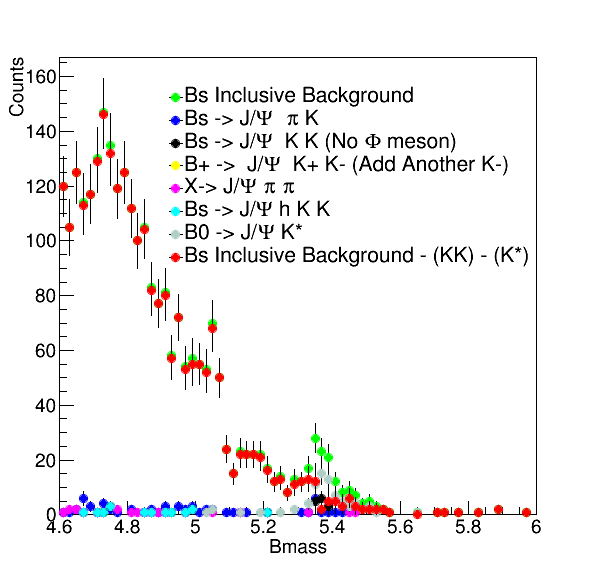
\includegraphics[width=0.45\linewidth]{Figures/Chapter5/NPBackgroundONLY_2.png}
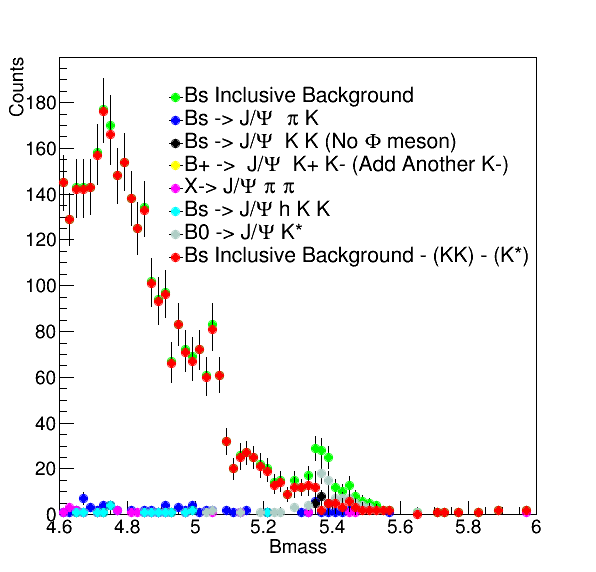
\includegraphics[width=0.45\linewidth]{Figures/Chapter5/NPBackgroundONLY_3.png}
\caption{Individual NP background contributions with respect to the total background components for 10 to 15 GeV (top left), 15 to 20 GeV (top right), 20 to 50 GeV (bottom left), and 10 to 50 GeV (bottom right) for PbPb sample. We can see that the non-prompt background from all channels listed above is negligible compared to the inclusive background. Also, no peak near the $B_s^0$ resonance is observed when the inclusive background subtracts the $B^0 \rightarrow J/\psi  K^{*0} $ and $B_s \rightarrow J/\psi  K^+ K^-$ components.}
\label{BsNPbkgd}
\end{figure}


Figure \ref{BsNPBS} also includes the signal component in the distribution. We can see that the non-prompt background is insignificant compared to the total inclusive background and the inclusive background is low comparing to the $B_s \rightarrow J/\psi \phi \rightarrow J/\psi K^+ K^-$ signal in our studies.
 
 
 
 \begin{figure}[ht!]
\centering
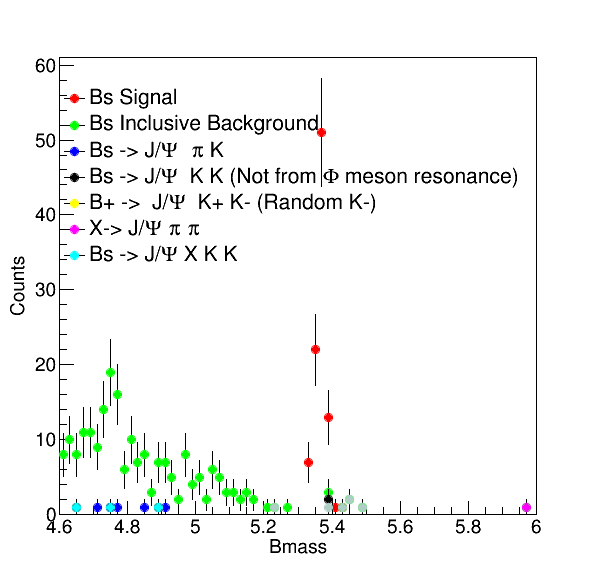
\includegraphics[width=0.45\linewidth]{Figures/Chapter5/NPBackground_0.png}
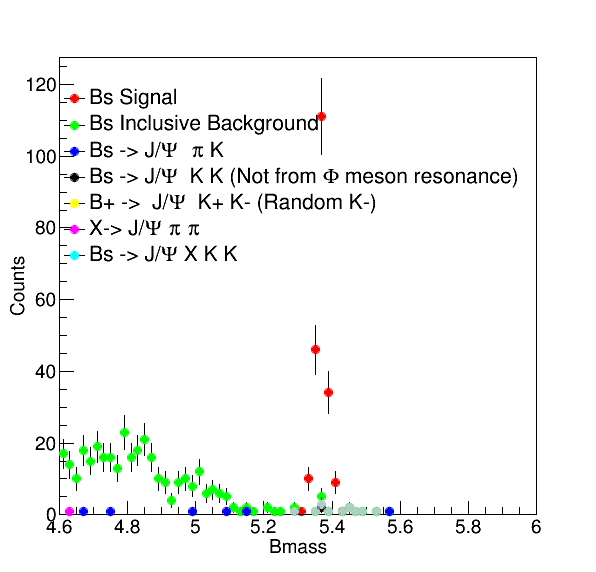
\includegraphics[width=0.45\linewidth]{Figures/Chapter5/NPBackground_1.png}
\includegraphics[width=0.45\linewidth]{Figures/Chapter5/NPBackground_2.png}
\includegraphics[width=0.45\linewidth]{Figures/Chapter5/NPBackground_3.png}
\caption{Individual Non Prompt background contributions with respect to the total background components and the signal channel for 10 to 15 GeV (top left), 15 to 20 GeV (top right), 20 to 50 GeV (bottom left), and 10 to 50 GeV (bottom right) for PbPb sample. We can see that the inclusive background is small compared to the signal we used in our studies.}
\label{BsNPBS}
\end{figure}
 
 
\subsection{B-meson contribution of NP Background to $B^0_s$}


From the non-prompt background studies above, we can see that there are many small contributions. Those small components together summed up constructing a large background and we can not identify all of them individually. Under this circumstances, another definition of individual component is used. The new definition of the NP background components are listed below;

\begin{itemize}
\item {Case 1: $ B^{+} \rightarrow J/\psi X $, all contributions from B+}
\item {Case 2: $ B_{s}^{0} \rightarrow J/\psi X $ , all contributions from $ B_{s}^{0} $ }
\item {Case 3: $ B^{0} \rightarrow J/\psi X$, all contributions from $ B^{0}$}
\item {Case 4: Other contributions}
\end{itemize}

In Figure \ref{BMesonNPCon} the signal region is dominated by the $B^{0}$, $B^{+}$, and $B_{s}^{0} $ decays while the other channels are contributed on the left side of the mass spectrum. For both $pp$ and PbPb data, the $B^{0}_{s} $ to $J/\psi$ + X  (orange region) makes a big contribution.

\begin{figure}[ht!]
\centering
\includegraphics[width=0.45\linewidth]{Figures/Chapter5/BmesonBackground_0.png}
\includegraphics[width=0.45\linewidth]{Figures/Chapter5/BmesonBackground_1.png}
\includegraphics[width=0.45\linewidth]{Figures/Chapter5/BmesonBackground_2.png}
\includegraphics[width=0.45\linewidth]{Figures/Chapter5/BmesonBackground_3.png}
\caption{ $B^{+}$, $B_{s}^{0} $, $ B^{0}$ channels make nearly equal contribution in the signal region for all $p_T$ bins 10 - 15 GeV/c, 15 - 20 GeV/c, 20 - 50 GeV/c, and 10 - 50 GeV/c.}
\label{BMesonNPCon}
\end{figure}

 

The conclusion is that the NP peaking background contribution to the $B^0_s$ is negligible due to the $K^{*0} (892)$ veto cut: $|m_{KK} - m_\phi| < 0.015$ GeV/c$^2$. We estimate that it may only contribute around 4\% uncertainties to the signal yield, which is negligible compared to the statistical uncertainties of the $B^0_s$ signal, which is on the order of 10\%. Hence, there is no need to develop a specific function to model the NP background component for $B^0_s$.


\subsection{B-meson contribution of NP Background to $B^+$}

We veto the candidates from the inclusive NP $J/\psi$ MC sample that are matched to a genuine $B^+$ signal. The resulting B candidate mass spectrum in the inclusive $p_T$ range (5-100 GeV/c) is shown in Figure \ref{NPBP} for PbPb MC samples. 

It is clear that these sources create a peaking structure in the region of $\rm M_{inv}<$5.20 GeV/c$^2$ as seen in Figure \ref{Bpeaks} after applying the optimal selection. This structure can be nicely fit with an error function as done previously in B-meson $pp$ analyses \cite{CMSBPH}. In addition, there is a minor peak on the right shoulder ($\approx$5.34 GeV/c$^2$) of the nominal signal ($\approx$5.28 GeV/c$^2$), and this can be fitted with a Gaussian function. The additional combinatorial background can be fitted with an exponential decay function. This contribution is absorbed in the total combinatorial background of our nominal channel of the main analysis. This will be described in detail in Section 4.6. The shape of the NP background model function is used as a template in the fit extraction procedure. 

Further MC studies have been done in order to identify the different channels that give rise to the non-prompt peaking structure in the $B^+$ invariant mass spectrum. Several main processes have been identified as follows:

\begin{itemize}
\item Case 1: 4-body $B^+$ decays which occur via resonant decay channels e.g. $B^+\rightarrow J/\psi K^{*+}(892)$. In these cases, we distinguish the kaons coming from the $K^{*+}(892)$ decays as coming from a signal $B^+\rightarrow J/\psi~K^+$ decay. 
\item Case 2: 4-body $B^0$ decays channels e.g. $B^0\rightarrow J/\psi K^{*0}(892)$.
\item Case 3: $B^+\rightarrow J/\psi\pi^+$ decays in which we have misidentified the $\pi^+$ as a $K^+$.
\end{itemize}

The different contributions in PbPb are presented in Fig.\ref{BPNPPeak}.
The contribution from $B^+\rightarrow J/\psi \pi$ clearly forms a peaking structure on the right shoulder of the nominal decay channel $B^+$ decay. However, the overall magnitude of this component is tiny compared to the other two sources, and negligible compared to the nominal signal. As a consequence, we can barely see the contribution of this peaking structure in the invariant mass plot of $B^+$ nominal channel.

\begin{figure}[h]
\begin{center}
\includegraphics[width= 0.45\textwidth]{Figures/Chapter5/fitNP_PbPb.pdf}
\caption{$B^+$ candidate mass spectrum obtained in inclusive B-meson MC production after vetoing the contribution of genuine $B^+$ signal candidates in PbPb.}
\label{NPBP}
\end{center}
\end{figure}

\begin{figure}[h]
\begin{center}
\includegraphics[width= 0.32\textwidth]{Figures/Chapter5/BmassBpPi.pdf}
\includegraphics[width= 0.32\textwidth]{Figures/Chapter5/BmassBpK_tkmatch.pdf}
\includegraphics[width= 0.32\textwidth]{Figures/Chapter5/BmassB0K_tkmatch.pdf}
\caption{Peaking background contribution from $B^+\rightarrow J/\psi \pi$ and from K resonant decay channels of $B^0$ and $B^+$ in PbPb MC.}
\label{BPNPPeak}
\end{center}
\end{figure}

The conclusion from these studies is that we need to use a function to model the NP background component. Its template shape should be determined according to the $B^+$ NP MC sample and applied to the data with a scale parameter. According to our studies, such function is the error function in the left-hand shoulder (low than the $B^+$ PDG mass) and a double Gaussian in the $B^+$ signal region.

\section{Signal Extraction} 

Now, equipped with the optimal selection and the NP background studies, we are ready to extract the signal raw yield from the B-meson invariant distribution and measure the cross section. Also, since we see very clear $B^0_s$ signals, we can estimate the $B^0_s$ significances and check if that leads to an observation.

\subsection{Fitting Models}

Raw yields are extracted through extended unbinned maximum likelihood fits the invariant mass of reconstructed $B^0_s$ meson candidates, performed using the \textit{Roofit} package \cite{ROOFIT}. The unbinned fit can reduce the potential bias due to the binning artifact. We develop the probability density function (PDF) to fit to the B-meson invariant mass distributions to extract their signal raw yields. In the PDF, the signal region for both $B^0_s$ and $B^+$ are described by Gaussian functions with the same means but different widths while the combinatorial background is modeled with an exponential decay function. For $B^+$, an additional error function in the left-hand shoulder (low than the $B^+$ PDG mass) and a double Gaussian in the $B^+$ signal region to fit NP peaking background due to the  b-hadron feed down based on the template fits to inclusive NP $J/\psi$ MC sample in Section 4.7. 

Hence, the generic event likelihood in data is described by the formula below

\begin{equation}
{\cal{L}}(m;N_S) = N_S \cdot (\alpha G(m;M,\sigma_1) + (1-\alpha) G(m; M,\sigma_2))+ N_B \cdot E(m;\lambda_m)
\end{equation}

\begin{equation}
G(m;M,\sigma) = \frac{1}{\sqrt{2\pi}\sigma} \exp^{-\frac{(m-M)^2}{2\sigma^2}} 
\end{equation}

\begin{equation}
E(m;\lambda_m) = \exp^{-\lambda_m m}
\end{equation}

Where $m$ is the candidate mass (input); $M$ and $\sigma_i$ are the signal mass means and widths (resolution); $G$ and $E$ denote respectively Gaussian and Exponential functions, normalized in the fitting mass window; $N_S$ denotes the signal raw yield (the parameter of interest),  $N_B$ is the background yield, while $\alpha$ and $\lambda_m$ are nuisance parameters (describing the signal fractions and exponential decay slope). %As mentioned already, $\alpha$, $\sigma_1$ and $\sigma_2$ are fixed from the MC fit.

It should note that the main reason for using double Gaussian functions instead of a single Gaussian is that the reconstructed $B^0_s$ signal width varies as a function of B-meson $pT$ due to the $p_T$ dependence of the track $p_T$ resolution. Figure \ref{BsBPWidthPT} shows the $B^0_s$ and $B^+$ invariant mass width as a function of $p_T$ in the MC


\begin{figure}[ht!]
\centering
\includegraphics[width=0.48\linewidth]{Figures/Chapter5/BsHisPtWidth.eps}
\includegraphics[width=0.48\linewidth]{Figures/Chapter5/BPHisPtWidth.eps}
\caption{The signal $B^0_s$ (left) and $B^+$ (right) invariant mass width as a function of $p_T$ are shown above.}
\label{BsBPWidthPT}
\end{figure}


\subsection{Raw Yield Extraction}


To obtain the signal raw yields and their statistical uncertainties from $B^0_s$ and $B^+$ invariant mass distribution, the following fitting procedures are carried out within B-meson invariant mass window $5 < m < 6$ GeV/c$^2$.

\begin{itemize}
\item First, a fit is performed, with a double Gaussian function to the MC invariant mass distribution of the genuine B-meson signals.
\item For $B^+$, the shape of the non-prompt background component is obtained using the dedicated non-prompt $J/\psi$ MC samples.
\item The fit is performed to the data with the fixed shapes (widths and relative proportion of the two Gaussians) same with the Gaussians obtained from the MC fit.
\item For systematic uncertainty check, add a free parameter ($a$), which is commonly multiplied by the widths of the signal Gaussians, serving as a scale factor of the resolution that parametrizes data and MC signal shape difference. However, in the nominal fit, this is set to be unity ($a = 1$), which means the widths of the data signal are set to be identical to the ones of the MC signal.
\item The parameters of the background PDF, the mean of the signal Gaussians are the free parameters of the fit.
\end{itemize}

% First, the fit is performed to the MC invariant mass distribution to obtain the two double Gaussian width parameters $\sigma_1$ and $\sigma_2$ as well as the relative proportion $\alpha$ describing the signal. Then, the fit is performed to the reconstructed B-meson invariant mass distribution in data, fixing the values of the $\sigma_1$ and $\sigma_2$ and the relative proportion $\alpha$ between the two gaussians to the value obtained from the MC fit. The mean of the Gaussian is treated as a floating parameter. The background components, including the NP peaking background and combinatorial background, are also determined according to the fit.

Figure \ref{BsMassPt} shows the fitting results of $B^0_s$ in the $p_T$ range of [7, 10, 15, 20, 50] GeV/c.  


\begin{figure}[h]
\begin{center}
\includegraphics[width= 0.45\textwidth]{Figures/Chapter5/data_PbPb_1_BptNew_710_doubly0_0_90EffInfoTreeFit.pdf}
\includegraphics[width= 0.45\textwidth]{Figures/Chapter5/data_PbPb_2_BptNew_1015_doubly0_0_90EffInfoTreeFit.pdf}
\includegraphics[width= 0.45\textwidth]{Figures/Chapter5/data_PbPb_3_BptNew_1520_doubly0_0_90EffInfoTreeFit.pdf}
\includegraphics[width= 0.45\textwidth]{Figures/Chapter5/data_PbPb_4_BptNew_2050_doubly0_0_90EffInfoTreeFit.pdf}
\caption{The $B^0_s$ invariant mass distributions as well as the fits to extract the signal raw yield $N_{S}$ in different $p_T$ bins are shown above.}
\label{BsMassPt}
\end{center}
\end{figure}

Figure \ref{BsMassCent} shows the fitting results of $B^0_s$ in the centrality range of [0, 30, 90] in PbPb collisions.  

\begin{figure}[h]
\begin{center}
\includegraphics[width= 0.45\textwidth]{Figures/Chapter5/data_PbPb_1_BptNew_1050_doubly0_0_30EffInfoTreeFit.pdf}
\includegraphics[width= 0.45\textwidth]{Figures/Chapter5/data_PbPb_1_BptNew_1050_doubly0_30_90EffInfoTreeFit.pdf}
\includegraphics[width= 0.45\textwidth]{Figures/Chapter5/data_PbPb_1_BptNew_1050_doubly0_0_90EffInfoTreeFit.pdf}
\caption{The $B^0_s$ invariant mass distributions as well as the fits to extract the signal raw yield $N_{S}$ in different centrality bins are shown above.}
\label{BsMassCent}
\end{center}
\end{figure}

Figure \ref{BPMassPt} shows the fitting results of $B^+$ in the $p_T$ range of [7, 10, 15, 20, 50] GeV/c.  


\begin{figure}[h]
\begin{center}
\includegraphics[width= 0.45\textwidth]{Figures/Chapter5/data_PbPb_1_Bpt_710_doubly0_0_90_ntKp.pdf}
\includegraphics[width= 0.45\textwidth]{Figures/Chapter5/data_PbPb_2_Bpt_1015_doubly0_0_90_ntKp.pdf}
\includegraphics[width= 0.45\textwidth]{Figures/Chapter5/data_PbPb_3_Bpt_1520_doubly0_0_90_ntKp.pdf}
\includegraphics[width= 0.45\textwidth]{Figures/Chapter5/data_PbPb_4_Bpt_2050_doubly0_0_90_ntKp.pdf}
\caption{The $B^+$ invariant mass distributions as well as the fits to extract the signal raw yield $N_{S}$ in different $p_T$ bins are shown above.}
\label{BPMassPt}
\end{center}
\end{figure}

Figure \ref{BPMassCent} shows the fitting results of $B^0_s$ in the centrality range of [0, 30, 90] in PbPb collisions.  

\begin{figure}[h]
\begin{center}
\includegraphics[width= 0.45\textwidth]{Figures/Chapter5/data_PbPb_1_Bpt_1050_doubly0_0_30_ntKp.pdf}
\includegraphics[width= 0.45\textwidth]{Figures/Chapter5/data_PbPb_1_Bpt_1050_doubly0_30_90_ntKp.pdf}
\includegraphics[width= 0.45\textwidth]{Figures/Chapter5/data_PbPb_1_Bpt_1050_doubly0_0_90_ntKp.pdf}
\caption{The $B^+$ invariant mass distributions as well as the fits to extract the signal raw yield $N_{S}$ in different centrality bins are shown above.}
\label{BPMassCent}
\end{center}
\end{figure}

Table \ref{BsRawYield} and \ref{BPRawYield} below summarize the selected fit parameters and their error extracted from the fits of $B^0_s$ and $B^+$ respectfully



\begin{table}[h]
\begin{center}
\caption{The summary table of $B^0_s$ fits results of Gaussian mean, signal raw yield, and background raw yield as well as their uncertainties.}
\vspace{1em}
\label{BsRawYield}
  \begin{tabular}{ |c|c|c|c|c|}
    \hline 
Centrality (\%) & $B^0_s$ $p_T$ (GeV/c) & Gaus Mean (GeV/c$^2$) & Sig Yield ($N_S$) & Bkgd Yield ($N_B$) \\
     \hline
0 -- 90 & 7 -- 10 & 5.386 $\pm$ 0.007 & 5.94 $\pm$ 2.43 & 1.06 $\pm$ 1.03 \\
0 -- 90 & 10 -- 15 & 5.368 $\pm$ 0.003 & 23.41 $\pm$ 5.28 & 35.59 $\pm$ 6.28 \\
0 -- 90 & 15 -- 20 & 5.369 $\pm$ 0.002 & 26.70 $\pm$ 5.31 & 16.33 $\pm$ 4.20 \\
0 -- 90 & 20 -- 50 & 5.371 $\pm$ 0.003 & 30.19 $\pm$ 5.73 & 16.82 $\pm$ 4.39 \\
0 -- 30 & 10 -- 50 & 5.369 $\pm$ 0.002 & 54.64 $\pm$ 7.86 & 60.35 $\pm$ 8.19 \\
30 -- 90 & 10 -- 50 & 5.370 $\pm$ 0.003 & 29.88 $\pm$ 5.58 & 10.13 $\pm$ 3.37 \\
0 -- 90 & 10 -- 50 & 5.369 $\pm$ 0.002 & 80.25 $\pm$ 9.43 & 68.74 $\pm$ 8.79 \\
     \hline
    \hline
\end{tabular}
\end{center}
\end{table}


\begin{table}[h]
\begin{center}
\caption{The summary table of $B^+$ fits results of Gaussian mean, signal raw yield, and background raw yield as well as their uncertainties.}
\vspace{1em}
\label{BPRawYield}
  \begin{tabular}{ |c|c|c|c|c|}
    \hline 
Centrality (\%) & $B^+$ $p_T$ (GeV/c) & Gaus Mean (GeV/c$^2$) & Sig Yield ($N_S$) & Bkgd Yield ($N_B$) \\
     \hline
0 -- 90 & 7 -- 10 & 5.277 $\pm$ 0.004 & 92.33 $\pm$ 10.88 & 7.90 $\pm$ 2.33 \\
0 -- 90 & 10 -- 15 & 5.279 $\pm$ 0.001 & 354.6 $\pm$ 20.68 & 39.9 $\pm$ 6.28 \\
0 -- 90 & 15 -- 20 & 5.279 $\pm$ 0.001 & 26.70 $\pm$ 5.31 & 16.33 $\pm$ 4.20 \\
0 -- 90 & 20 -- 50 & 5.278 $\pm$ 0.001 & 30.19 $\pm$ 5.73 & 16.82 $\pm$ 4.39 \\
0 -- 30 & 10 -- 50 & 5.278 $\pm$ 0.001 & 657.7 $\pm$ 27.7 & 53.46 $\pm$ 5.28 \\
30 -- 90 & 10 -- 50 & 5.281 $\pm$ 0.001 & 327.0 $\pm$ 19.5 & 19.57 $\pm$ 4.69 \\
0 -- 90 & 10 -- 50 & 5.279 $\pm$ 0.001 & 971.6 $\pm$ 33.9 & 74.16 $\pm$ 6.91 \\
     \hline
 \end{tabular}
\end{center}
\end{table}

At a glance, we can see that our fits all look good. In addition to the fits, the pull, defined as the ratio of the difference between the data and the fit to the statistical uncertainties of the data, are also shown above in Figure \ref{BsMassPt}, Figure \ref{BsMassCent}, Figure \ref{BPMassPt}, and Figure \ref{BPMassCent}. We can see that the pull is basically consistent with 0 with a 2$\sigma$ fluctuation, which suggests that our fit also looks good. A dedicated closure test on the fits will be conducted later to further validate our fits.

\subsection{Signal Significance Estimation}

The significance (Z) is calculated through a likelihood method, which follows the formula below:

\begin{equation}
Z=\sqrt{ 2 \log \frac{L_{S+B}}{L_B}}
\end{equation}

Here, $L_{S+B}$ is the likelihood of each fit and $L_B$ is the likelihood when the number of signal $N_S$ parameter is fixed to 0. Figure \ref{BsSigScan} show the likelihood scan of $B^0_s$ in 4 $p_T$ bins and 3 centrality bins

\begin{figure}[h]
\begin{center}
\includegraphics[width= 0.45\textwidth]{Figures/Chapter5/sigscan_0_90_7_10.png}
\includegraphics[width= 0.45\textwidth]{Figures/Chapter5/sigscan_0_90_10_15.png}
\includegraphics[width= 0.45\textwidth]{Figures/Chapter5/sigscan_0_90_15_20.png}
\includegraphics[width= 0.45\textwidth]{Figures/Chapter5/sigscan_0_90_20_50.png}
\caption{The significance vs signal yield for $p_T$ bins at 7 -- 10, 10 -- 15, 15 -- 20, and 20 -- 50 GeV/c for 0 - 90\% centrality are shown above}
\label{BsSigScan}
\end{center}
\end{figure}


\begin{figure}[h]
\begin{center}
\includegraphics[width= 0.45\textwidth]{Figures/Chapter5/sigscan_0_30_10_50.png}
\includegraphics[width= 0.45\textwidth]{Figures/Chapter5/sigscan_30_90_10_50.png}
\includegraphics[width= 0.45\textwidth]{Figures/Chapter5/sigscan_0_90_10_50.png}
\caption{The significance vs signal yield for centrality bins in 0 - 30\%, 30\% - 90\% 0 - 90\% for $p_T$ in 10 - 50 GeV/c are shown above}
\label{fig:SigScanCent}
\end{center}
\end{figure}



Table \ref{BsSig} summarizes the significance of $B^0_s$ according to our likelihood estimation.



\begin{table}[h]
\begin{center}
\caption{The summary table of $B^0_s$ likelihood significance for each $p_T$ and centrality bin.}
\vspace{1em}
\label{BsSig}
  \begin{tabular}{ |c|c|c|}
    \hline 
Centrality (\%) & $B^0_s$ $p_T$ (GeV/c) & Likelihood Significance (Z)  \\
     \hline
0 -- 90 & 7 -- 10 & 5.3 \\
0 -- 90 & 10 -- 15 & 7.9 \\
0 -- 90 & 15 -- 20 & 10 \\
0 -- 90 & 20 -- 50 & 10 \\
0 -- 30 & 10 -- 50 &  14 \\
30 -- 90 & 10 -- 50 &  11\\
0 -- 90 & 10 -- 50 & 16 \\
     \hline
    \hline
\end{tabular}
\end{center}
\end{table}



We can see that $B^0_s$ mesons have significances of greater than 5$\sigma$ for all its $p_T$ and centrality bins. In fact, this is the first observation of fully reconstructed $B^0_s$ meson in nucleus-nucleus collisions with greater than 5$\sigma$ significance. 

\section{B Mesons Candidates MC-Data Comparison}

\subsection{overview}

Ideally, if the simulation is impeccable, the RECO distribution in the MC should match perfectly with the data. Nevertheless, there is always a limitation in the MC simulation because of the incorrect modeling of physics processes in the generation side or poor implementation of detector effects on the reconstruction side. The discrepancy should be quantified as a source of systematic uncertainties. The MC simulation plays a crucial role in the data analysis and could affect our final results significantly. In order to compare the consistency between data and MC, we need to look at the B-meson signal-only candidates. In the MC, we can simply apply GEN Match selection to select all B-meson signal candidates. In the data, we need to reject the background and extract the signal. After that, we compare the normalized distributions of the data and MC to compare their shapes. 

\subsection{\textbf{Splot} Techniques}

To carry out MC-Data comparison studies, the dedicated \textit{Splot} method is used. It is a likelihood-based method by which we reweigh the data using the unbinned fit result. The weights are added to the dataset based on model and yield extraction variables. Each event has two weights: the probability of belonging to the signal given its mass, probability of belonging to the background given its mass. The \textit{Splot} class gives us the distributions of our variables for a given species (signal or background). The advantage of using this method is that we use the full dataset for the comparison in contrast to the sideband subtraction method where one should select the investigation range of signal and background. Furthermore, we use likelihood to describe events' behavior in contrast to the potential misidentification of signal events in the background region which might occur in the sideband subtraction method. 

%ADD DESCRIPTIONS OF SPLOT TECHNIQUE HERE BRO

In order to obtain the \textit{Splot} weight, we first need to fit the data using a discriminating variable, namely the B-meson candidates invariant mass. This method, like the one described in the previous section, assumes the discriminating variable chosen to be independent of the variables we wish to study. We then use the fit to attribute to each event two weights: $w_{S}$, which corresponds to the probability of it belonging to the signal, and $w_B$, which corresponds to the probability of fit belonging to the background. The weights are qualitatively demonstrated in Figure \ref{SplotPic}.


\begin{figure}[h]
\begin{center}
\includegraphics[width=0.75\textwidth]{Figures/Chapter5/SplotWeighPic.png}
\caption{The illustration of \textit{Splot} techniques via an unbinned fit to $B^+$ invariant mass distribution using our fitting model to extract the \textit{Splot} weights $w_S$ and $w_B$ is shown above.}
\label{SplotPic}
\end{center}
\end{figure}


\subsection{\textbf{Splot} Variable Correlation Studies}

First, in order to apply Splot to perform Data-MC comparison, we need to confirm our variables are indeed not correlated to the invariant mass. Therefore, the correlation matrices for BDT variables vs $B^+$ invariant mass (Bmass) for data and MC are shown in Figure~\ref{BPBDTCorr}:


\begin{figure}[h]
\begin{center}
\includegraphics[width=0.45\textwidth]{Figures/Chapter5/BsBDTCorrB.pdf}
\includegraphics[width=0.45\textwidth]{Figures/Chapter5/BsBDTCorrB.pdf}
\caption{The correlation matrices in data (left) and MC (right) of $B^0_s$ are shown above.}
\label{BsBDTCorr}
\end{center}
\end{figure}

\begin{figure}[h]
\begin{center}
\includegraphics[width=0.45\textwidth]{Figures/Chapter5/BPBDTCorrB.pdf}
\includegraphics[width=0.45\textwidth]{Figures/Chapter5/BPBDTCorrS.pdf}
\caption{The correlation matrices in data (left) and MC (right) of $B^+$ are shown above.}
\label{BPBDTCorr}
\end{center}
\end{figure}

\subsection{\textbf{Splot} Results for Data-MC Comparison}



No significant correlation between the BDT variables and the invariant mass is observed in either $B^0_s$ and $B^+$, which also validates their BDT training. Therefore, \textit{Splot} will be applicable to compare data and MC. Here, we focus on BDT values that are directly used in our signal extraction and related to MC distribution validation, rather than the variables themselves used in BDT training. In a wide range of BDT, the two distributions show good agreement. We only focus on the region where BDT is greater than the working point and is smaller than the maximum value that candidates have.

\begin{figure}[h]
\begin{center}
\includegraphics[width=0.45\textwidth]{Figures/Chapter5/Bs_BDT_5_10.png}
\includegraphics[width=0.45\textwidth]{Figures/Chapter5/Bs_BDT_10_15.png}
\includegraphics[width=0.45\textwidth]{Figures/Chapter5/Bs_BDT_15_20.png}
\includegraphics[width=0.45\textwidth]{Figures/Chapter5/Bs_BDT_20_50.png}
\caption{Comparison of $B^0_s$ BDT distribution in data (red) and MC (green) using the \textit{Splot} method.}
\label{BsMCData}
\end{center}
\end{figure}

\begin{figure}[h]
\begin{center}
\includegraphics[width=0.45\textwidth]{Figures/Chapter5/BDT_pt_5_7_mc_validation_Bu.pdf}
\includegraphics[width=0.45\textwidth]{Figures/Chapter5/BDT_pt_7_10_mc_validation_Bu.pdf}
\includegraphics[width=0.45\textwidth]{Figures/Chapter5/BDT_pt_10_15_mc_validation_Bu.pdf}
\includegraphics[width=0.45\textwidth]{Figures/Chapter5/BDT_pt_15_20_mc_validation_Bu.pdf}
\includegraphics[width=0.45\textwidth]{Figures/Chapter5/BDT_pt_20_30_mc_validation_Bu.pdf}
\includegraphics[width=0.45\textwidth]{Figures/Chapter5/BDT_pt_30_40_mc_validation_Bu.pdf}
\includegraphics[width=0.45\textwidth]{Figures/Chapter5/BDT_pt_40_50_mc_validation_Bu.pdf}
\includegraphics[width=0.45\textwidth]{Figures/Chapter5/BDT_pt_50_60_mc_validation_Bu.pdf}
\caption{Comparison of $B^+$ BDT distribution in data (red) and MC (green) using the \textit{Splot} method.}
\label{BPMCData}
\end{center}
\end{figure}

From Figure \ref{BPMCData}, the $B^+$ BDT variables in for all $p_T$ bins have overall reasonably good agreement between Data and MC. Their ratio is near unity with some fluctuations due to limited statistics. In the systematic section, we will quantify the discrepancy between Data and MC as a source of systematic uncertainties. For $B^0_s$, unlike $B^+$ whose statistics is in general $>$ 100, the total number of signal $B^0_s$ candidates is $<$ 100, which results in a large error bar shown in Figure \ref{BsMCData}. Nonetheless, the ratio of Data to MC shape is still near unity within the large uncertainties. Nevertheless, since the events used by $B^0_s$ and $B^+$ are essentially the same and their tracks are very similar, the overall good $B^+$ Data-MC agreement can provide indirect validation to $B^0_s$. The CMS analysis note AN-19-219 \cite{AN-19-219} documents more details on the general description of the \textit{Splot} method applied to this analysis.  


\section{Acceptance and Efficiency Correction} 

\subsection{Overview}

Now, we have clearly seen B-meson signals and extract their signal raw yields $N_S$ from their invariant distributions. In the next step, we need to correct the acceptance and selection efficiency of the B mesons in order to obtain the cross section. The following procedures define the method we use to determine B mesons acceptance and selection efficiency with B-meson MC samples:

First, We count the total number of GEN-level B-meson candidates reweighed by the centrality, PV$_{z}$, and $\hat p_T$ as \textbf{NBGen} within the given B-meson rapidity region $|y| < 2.4$.

Next, we count the number of generated B-meson candidates passing the following selections

\textbf{Muon track selections:}

\begin{equation}
\centering
\setlength\arraycolsep{20pt}
\begin{array}{l c r r}
p_T^{\mu}>3.5 GeV/c & & \text{for}\enspace |\eta^{\mu}|<1.2 & \\
p_T^{\mu}>(5.47 - 1.89\times |\eta^{\mu}|) GeV/c & &  \text{for}\enspace 1.2\le |\eta^{\mu}|<2.1 &\\
p_T^{\mu}>1.5 GeV/c & & \text{for}\enspace 2.1\le |\eta^{\mu}|<2.4 &
\end{array}
\label{eq:SingleMuonAccCuts}
\end{equation}


\textbf{Kaon track selections:}

\begin{equation}
\centering
\setlength\arraycolsep{20pt}
\begin{array}{l c r r}
p_T^{K}>0.9 GeV/c \\
|\eta^{K}| < 2.4
\end{array}
\label{eq:KaonTrackCut}
\end{equation}

We denote those generated B-meson candidates passing selections as \textbf{NPassAcc}.


Finally, we apply all the selections on the GEN-matched RECO B mesons. We count the reconstructed B-meson candidates passing the selections mentioned in Section 4.5 ``Muon and $J/\psi$ candidates selections" and the optimal BDT selections in Table 3 in Section 4.1 and denote the number as \textbf{NSelPass}.

The acceptance is defined by: \textbf{acceptance = NPassAcc/NBGen}.

The selection efficiency is defined by: \textbf{selection efficiency = NSelPass/NPassAcc}.

Here, we denote $\alpha$ \textbf{as the acceptance} and $\epsilon$ \textbf{as the selection efficiency} and their product, which is \textbf{$\alpha \times \epsilon$ = NSelPass/NBGen}, is call (total) efficiency. 

\subsection{Tag \& Probe Techniques}

The previous subsection mentioned the efficiency correct for B-meson using MC simulations only. However, we know that both $B^0_s$ and $B^+$ decay to $J/\psi$. A dedicated analysis technique called tag \& probe is developed to correct the B-meson efficiency in a data-driven way. The tag-\&-probe method uses the \textit{scale factor} defined as the ratio of Data/MC for L2 and L3 triggered single muon efficiency tagged from the $J/\psi$ resonance \cite{TnPMethod}. There are three scale factors: identification (id), tracking (trk), and trigger (trg). Figure \ref{L2L3MuonWF} shows the workflow for tag-\&-probe in B-meson analysis


\begin{figure}[h]
\begin{center}
\includegraphics[width= 0.85\textwidth]{Figures/Chapter5/L2L3MuonWF.pdf}
\caption{The workflow to obtain L2 and L3 muons in order to apply the tag-\&-probe method.}
\label{L2L3MuonWF}
\end{center}
\end{figure}

The total scale factor (SF) of two muons ($SF^{\mu\mu}$) is given by the following formula

\begin{equation}
SF^{\mu\mu} = id^{\mu_1} \times trk^{\mu_1}  \times trg^{\mu_1}  \times id^{\mu_2}  \times trk^{\mu_2}  \times trg^{\mu_2} 
\end{equation}

It should note that, as mentioned in Section 2.2.5, the dimuon PbPb triggered datasets consistent with one L2 muon and one L3 muon. In our analysis, the two muons used to reconstruct B-meson are made of either one L2 muon and one L3 muon (L2, L3) or two L3 muons (L3, L3). The muon type L2 and L3 only affect the trg SF. In the (L2, L3) case, we simply correct the scale factor according to their individual scale factor values. However, in the (L3, L3) case, we can treat them as the combination of (L2, L3) and (L3, L2) by considering one of the muon legs as L2 muon. Then we compute the SF for both cases and take the average of the two SF as the SF for (L3, L3).  

\subsection{Traditional Efficiency Correction Results}

Traditionally, we simply compute the efficiency as a function of binned $p_T$ and centrality and use it to correct the signal raw yield within the $p_T$ and centrality bins. The $B^0_s$ and $B^+$ acceptance, selection efficiency, and total efficiency as a function of $p_T$ and centrality are shown respectfully below in Figure \ref{BsEffAll} and Figure \ref{BPEffAll}

\begin{figure}[h]
\begin{center}
\includegraphics[width=0.48\textwidth]{Figures/Chapter5/BsAcc1DPtHis.png}
\includegraphics[width=0.48\textwidth]{Figures/Chapter5/BsAcc1DCentHis.png}
\includegraphics[width=0.48\textwidth]{Figures/Chapter5/BsSel1DPtHis.png}
\includegraphics[width=0.48\textwidth]{Figures/Chapter5/BsSel1DCentHis.png}
\includegraphics[width=0.48\textwidth]{Figures/Chapter5/BsEff1DPtHis.png}
\includegraphics[width=0.48\textwidth]{Figures/Chapter5/BsEff1DCentHis.png}
\caption{The $B^0_s$ acceptance (top), selection efficiency (middle), and efficiency (bottom) as a function of $p_T$ (left) and event centrality (right) are shown respectfully above. We should note that there is no significant centrality dependence on the $B^0_s$ acceptance, which makes sense.}
\label{BsEffAll}
\end{center}
\end{figure}


\begin{figure}[h]
\begin{center}
\includegraphics[width=0.48\textwidth]{Figures/Chapter5/BPAcc1DPtHis.png}
\includegraphics[width=0.48\textwidth]{Figures/Chapter5/BPAcc1DCentHis.png}
\includegraphics[width=0.48\textwidth]{Figures/Chapter5/BPSel1DPtHis.png}
\includegraphics[width=0.48\textwidth]{Figures/Chapter5/BPSel1DCentHis.png}
\includegraphics[width=0.48\textwidth]{Figures/Chapter5/BPEff1DPtHis.png}
\includegraphics[width=0.48\textwidth]{Figures/Chapter5/BPEff1DCentHis.png}
\caption{The $B^+$ acceptance (top), selection efficiency (middle), and efficiency (bottom) as a function of $p_T$ (left) and event centrality (right) are shown respectfully above. We should note that there is no significant centrality dependence on the $B^+$ acceptance, which makes sense.}
\label{BPEffAll}
\end{center}
\end{figure}


\subsection{Analysis Challenges}

Although B-meson $p_T$ and $y$ distributions are reasonably modeled by FONLL in $pp$ collisions, the precise B-meson $p_T$ and $y$ distribution shapes are still unknown in PbPb, which could significantly affect the efficiency determination. In the following, we demonstrate the generated B-meson kinematics how the unknown shape can affect the efficiency. 

Since we know the efficiency is given by \textbf{$\alpha \times \epsilon$ = NSelPass/NBGen}. NBGen in the simulation could not represent the truth. A weight function $w(x)$ is defined as the ratio between the generated B-meson cross section to the cross section of actual B-meson in PbPb for some kinematic variable $x$ as follows

\begin{equation}
w(x) = \frac{\sigma^{MC}_B (x)}{\sigma^{PbPb}_B (x)}
\end{equation}

Therefore, this weight function needs to be applied to both GEN-level $G(x)$ and RECO-level $R(x)$ in order to obtain the correct selection efficiency as a function of B mesons $p_T$. 


\begin{equation}
\epsilon_{corr}(x) =  \frac{\langle R(x) \rangle}{\langle G(x) \rangle}= \frac{\int R(x) w(x)dx}{\int G(x) w(x)dx}
\end{equation}

Experimentally, the data are discreet. Therefore, the measurement is done in bins. Now considering a bin of [$x_1,x_2$], the expression above is written as 

\begin{equation}
\epsilon_{corr}(x_1 < x < x_2) =  \frac{\int^{x_2}_{x_1} R(x) w(x)dx}{\int^{x_2}_{x_1} G(x) w(x)dx}
\end{equation}


When $x_1 \rightarrow x_2$, we have

\begin{equation}
\epsilon_{corr}(x_1 < x < x_2) =  \frac{\int^{x_2}_{x_1} R(x) w(x)dx}{\int^{x_2}_{x_1} G(x) w(x)dx} \sim  \frac{R(x) w(x)  (x_2 - x_1)}{G(x) w(x) (x_2 - x_1)}  = \frac{R(x)}{G(x)} = \epsilon(x)
\end{equation}

We can see that, for any non-trivial $w(x)$, with very fine bins, the effect of $w(x)$ is gone. When we measure B-meson over a large $p_T$ range, this effect could be significant, particularly for the $B^0_s$ mesons where the change of efficiency between 7 -- 10 GeV/c and 10 -- 15 GeV/c and the slope of uncertainties on $w(x)$ both are huge. Hence, in order to eliminate the uncertainties due to the B-meson kinematics $w(x)$ on efficiency correction, we can bin the efficiency finely.

\subsection{Fiducial Measurement}

In fact, to better estimate B-meson efficiency, we should use 2D efficiency maps as functions of B-meson $p_T$ and $|y|$. Figure \ref{Bs2DRECO} shows reconstructed $B^0_s$ and $B^+$ distribution in the MC

\begin{figure}[h]
\begin{center}
\includegraphics[width= 0.48\textwidth]{Figures/Chapter5/hBptByData.png}
\includegraphics[width= 0.48\textwidth]{Figures/Chapter5/hBptByMC.png}
\caption{The finely binned 2D candidates distribution vs B $p_T$ and B $|y|$ for data and MC at centrality 0 - 90\% are shown respectfully above.}
\label{Bs2DRECO}
\end{center}
\end{figure}

For B-meson $p_T$ below 10 GeV/c, very few B mesons are reconstructed at the rapidity region of $|y| < 1.5$. This is due to the limited acceptance of muons because the muon tracks at low $p_T$ cannot reach the muon systems. Hence, a fiducial measurement is carried out. We only correct B-meson for $p_T < 10$ GeV/c to the $1.5 < |y| < 2.4$ instead of $|y| < 2.4$. For $p_T > 10$ GeV/c, we still correct them to $|y| < 2.4$. The fiducial B-meson measurements will be carried out throughout this thesis.

\subsection{Finely Binned 2D Efficiency Map}

After unknown B-meson kinematics effects on efficiency correction and choosing the fiducial region for our measurement, we propose to measure the inverse of the total efficiency: $\frac{1}{\alpha \times \epsilon}$ as a function of $p_T$ and $|y|$ to correct the B-meson raw yield to production yield. We implement the following workflow in Figure \ref{EffWorkFlow} to estimate $\langle \frac{1}{\alpha \times \epsilon} \rangle$


\begin{figure}[h]
\begin{center}
\includegraphics[width= 0.85\textwidth]{Figures/Chapter5/EffCorrMethod.pdf}
\caption{The workflow for the efficiency correction including the data-driven tag-\&-probe approach in B-meson analysis is shown above.}
\label{EffWorkFlow}
\end{center}
\end{figure}

The $\frac{1}{\alpha \times \epsilon}$ applied with the tag-\&-probe SFs as functions of $p_T$ and $|y|$ for $B^0_s$ and $B^+$ are shown on Figure \ref{Bs2DMap} and Figure \ref{BP2DMap} respectfully 

\begin{figure}[h]
\begin{center}
\includegraphics[width= 0.32\textwidth]{Figures/Chapter5/BsEff2D_0_90.png}
\includegraphics[width= 0.32\textwidth]{Figures/Chapter5/BsEff2D_0_30.png}
\includegraphics[width= 0.32\textwidth]{Figures/Chapter5/BsEff2D_30_90.png}
\caption{The finely binned 2D $\frac{1}{\alpha \times \epsilon}$ vs $B^0_s$ $p_T$ and B $|y|$ for 0 - 90\% (top), 0 - 30\% (middle), and 30\% - 90\% (bottom) centrality are shown respectfully above.}
\label{Bs2DMap}
\end{center}
\end{figure}

\begin{figure}[h]
\begin{center}
\includegraphics[width= 0.32\textwidth]{Figures/Chapter5/BPEff2D_0_90.png}
\includegraphics[width= 0.32\textwidth]{Figures/Chapter5/BPEff2D_0_30.png}
\includegraphics[width= 0.32\textwidth]{Figures/Chapter5/BPEff2D_30_90.png}
\caption{The finely binned 2D $\frac{1}{\alpha \times \epsilon}$ vs $B^+$ $p_T$ and B $|y|$ for 0 - 90\% (top), 0 - 30\% (middle), and 30\% - 90\% (bottom) centrality are shown respectfully above.}
\label{BP2DMap}
\end{center}
\end{figure}

The $p_T$ bin width is 0.5 GeV/c from 5 - 10 GeV/c and 1 GeV/c from 10 - 50 GeV/c. The $|y|$ binning is [0, 1.2, 1.8, 2.1, 2.4].

\subsection{Data-Drive Efficiency Correction}

Finally, we propose to correct the efficiency with a data-driven method. We correct the signal B-meson candidate efficiency. This can be done by looping B-meson data signal region candidates on the 2D $\frac{1}{\alpha \times \epsilon}$ map according to their $p_T$ and $|y|$. Then, referring to techniques of the published $J/\psi$ analysis \cite{TnPMethod}, we compute the average of all signal B-meson candidate efficiency: $\langle\frac{1}{\alpha \times \epsilon} \rangle$ within the $p_T$ and centrality bins. Here, we call $\langle\frac{1}{\alpha \times \epsilon} \rangle$ as the efficiency correction factor. Mathematically, it is written as

\begin{equation}
\langle\frac{1}{\alpha \times \epsilon} \rangle = \frac{1}{N} \sum_{i = 1}^{N} \frac{1}{\alpha_i \times \epsilon_i}
\end{equation}

It should note that we will measure  $\langle\frac{1}{\alpha \times \epsilon} \rangle$ instead of $\frac{1}{\langle\alpha \times \epsilon \rangle}$ is because $\langle\frac{1}{\alpha \times \epsilon} \rangle$ has better closure. A dedicated closure test on this approach will be carried out and the results discussed the Section 4.11. 

Also, there are background contaminations even within the signal region. This could be improved by the \textit{Splot} method. However, it turns out that the difference in the efficiency between applying Splot and not applying Splot is very small. We do not consider using the \textit{Splot} method in this measurement. 

Finally, this method only gives nominal results. The statistical uncertainties turn out to be correlated with both the data and MC statistics. A dedicated data bootstrapping approach to estimate the statistical uncertainties of the efficiency correction factor $\frac{1}{\langle\alpha \times \epsilon \rangle}$ will be carried out in Section 4.12.

\subsection{Results}

After applying a data-driven method to compute the efficiency correction factor, we obtain Figure \ref{BsEffFig} and Figure \ref{BPEffFig} showing $\langle\frac{1}{\alpha \times \epsilon} \rangle$ as a function $p_T$ and centrality for both $B_s^0$ and $B^+$.


\begin{figure}[h]
\begin{center}
\includegraphics[width= 0.32\textwidth]{Figures/Chapter5/EffPlotPt.pdf}
\includegraphics[width= 0.32\textwidth]{Figures/Chapter5/EffPlotCent.pdf}
\includegraphics[width= 0.32\textwidth]{Figures/Chapter5/EffPlotCentInc.pdf}
\caption{The $B^0_s$ efficiency correction factor $\langle\frac{1}{\alpha \times \epsilon} \rangle$ vs $p_T$ (left) and 0 -- 30 \% and 30 -- 90\% centrality (middle) and the inclusive 0 -- 90\% centrality (right) are shown above.}
\label{BsEffFig}
\end{center}
\end{figure}

\begin{figure}[h]
\begin{center}
\includegraphics[width= 0.32\textwidth]{Figures/Chapter5/BPEffPlotPt.pdf}
\includegraphics[width= 0.32\textwidth]{Figures/Chapter5/BPEffPlotCent.pdf}
\includegraphics[width= 0.32\textwidth]{Figures/Chapter5/BPEffPlotCentInc.pdf}
\caption{The  $B^+$ efficiency correction factor $\langle \frac{1}{\alpha \times \epsilon} \rangle$ vs $p_T$ (left) and 0 -- 30 \% and 30 -- 90\% centrality (middle) and the inclusive 0 -- 90\% centrality (right) are shown above.}
\label{BPEffFig}
\end{center}
\end{figure}




Table \ref{BsEffTab} and \ref{BPEffTab} summarize the nominal efficiency of $B^0_s$ and $B^+$ respectfully and their upper and lower asymmetric statistical uncertainties obtained from Section 4.12.
%\section{Cross Section Results} 


\begin{table}[h]
\begin{center}
\caption{The summary table of $B^0_s$ efficiency correction factor $\langle\frac{1}{\alpha \times \epsilon} \rangle$ for each $p_T$ and centrality bin.}
\vspace{1em}
\label{BsEffTab}
  \begin{tabular}{ |c|c|c|c|c|}
    \hline 
Centrality (\%) & $B^0_s$ $p_T$ (GeV/c) & $\langle\frac{1}{\alpha \times \epsilon} \rangle$ & $\langle\frac{1}{\alpha \times \epsilon} \rangle$ Error Up +) &$\langle\frac{1}{\alpha \times \epsilon} \rangle$ Error Down -) \\
     \hline
0 -- 90 & 7 -- 10 & 381.5  &  19.3\% & 20.3\% \\
0 -- 90 & 10 -- 15 & 75.92 &  12.4\% & 12.3\% \\
0 -- 90 & 15 -- 20 & 22.35 &   6.41\% & 6.47\% \\
0 -- 90 & 20 -- 50 & 10.63 & 5.90\% &  6.20\% \\
0 -- 30 & 10 -- 50 & 45.90 & 14.9\% & 14.6\%  \\
30 -- 90 & 10 -- 50 & 14.19 & 10.3\% & 9.78\% \\
0 -- 90 & 10 -- 50 & 34.90 & 17.9\% & 16.3\% \\
     \hline
    \hline
\end{tabular}
\end{center}
\end{table}


\begin{table}[h]
\begin{center}
\caption{The summary table of $B^+$ efficiency correction factor $\frac{1}{\langle\alpha \times \epsilon \rangle}$ for each $p_T$ and centrality bin.}
\vspace{1em}
\label{BPEffTab}
  \begin{tabular}{ |c|c|c|c|c|}
    \hline 
Centrality (\%) & $B^+$ $p_T$ (GeV/c) &$\langle\frac{1}{\alpha \times \epsilon} \rangle$ & $\langle\frac{1}{\alpha \times \epsilon} \rangle$ Error Up +) & $\langle\frac{1}{\alpha \times \epsilon} \rangle$ Error Down -) \\
     \hline
0 -- 90 & 7 -- 10 & 105.9  &  15.8\% & 15.1\% \\
0 -- 90 & 10 -- 15 & 37.55 &  4.10\% & 7.95\% \\
0 -- 90 & 15 -- 20 & 10.94 &   6.54\% & 6.50\% \\
0 -- 90 & 20 -- 50 & 5.932 & 6.90\% &  5.26\% \\
0 -- 30 & 10 -- 50 & 21.67 & 5.81\% & 5.54\%  \\
30 -- 90 & 10 -- 50 & 12.28 & 6.71\% & 7.06\% \\
0 -- 90 & 10 -- 50 & 19.23 & 5.06\% & 4.54\% \\
     \hline
    \hline
\end{tabular}
\end{center}
\end{table}

At this point, we have all the ingredients to measure the B-meson cross section and study the physics. 

\section{Cross Section Measurement} 

The goal is this thesis is to measure the cross section of B-meson in PbPb collisions as functions of B mesons $p_T$ and PbPb collision event centrality. Here, in high-energy heavy-ion physics, cross section really means production yield. 

In terms of B mesons $p_T$, the cross section is defined mathematically as follows:

\begin{equation}
\frac{1}{T_{AA}}\frac{dN}{d p_T} =  \frac{1}{T_{AA}} \frac{1}{2} \frac{1}{\Delta p_T} \frac{1}{N_{MB} BR } N_S \langle\frac{1}{\alpha \times \epsilon} \rangle
\end{equation}

In terms of PbPb collision event centrality, the cross section is defined as mathematically as follows:

\begin{equation}
\frac{1}{T_{AA}} N =  \frac{1}{T_{AA}} \frac{1}{2} \frac{1}{N_{MB} BR} N_S \langle\frac{1}{\alpha \times \epsilon} \rangle
\end{equation}

The definitions of the variables above are shown below:

\begin{itemize}
\item $N$: B-meson production yield
\item $T_{AA}$: nuclear overlapping function - here is for spherical nucleus ${}^{208}_{82}$Pb  
\item $N_{MB}$: number of minimum biased events corresponding to the dimuon PbPb datasets
\item $\frac{1}{2}$: divide by 2 for the purpose of normalizing particle and antiparticle 
\item $BR$: B-meson decay branching ratio
%\item $f(b\rightarrow B)$: Beauty quark fragmentation fraction to B mesons
\item $\Delta p_T$: B-meson transverse momentum bin width
\item $N_S$: signal raw yield 
\item $\langle\frac{1}{\alpha \times \epsilon} \rangle$: the data-drive efficiency correction factor
\end{itemize}

It should be pointed out that we aim at measuring the $p_T$ differential cross section as a function B mesons $p_T$ while as we plan to present the $p_T$ integrated cross section as a function of event centrality in this thesis. Before presenting our final results of the cross section measurement, we need to validate our signal raw yield $N_S$ and efficiency correction factor $\langle\frac{1}{\alpha \times \epsilon} \rangle$ measurements and estimate the correct statistical and systematic uncertainties of the B-meson measurements. 

\section{Validation Tests} 

Before presenting the final results, some more validation tests need to complete to ensure our results are unbiased.

\subsection{Mass Scraping Test}

From Figure \ref{BsBDTCorr}, we see that the BDT variables are essentially uncorrelated to the $B^0_s$ invariant mass. However, uncorrelation is not equivalent to independence. We need to make sure that in the BDT training procedure, no significant invariant mass dependence is introduced. This effect is called the mass scraping effect. Therefore, we propose the following tests to explicitly quantify the $B^0_s$ BDT variables dependence on the $B^0_s$ invariant mass. 

\begin{itemize}
\item We look at the BDT shape in different $B^0_s$ data invariant mass sideband regions (both left- and right-hand side) that are far away from the $B^0_s$ PDG mass.
\item Then we take the ratio from other BDT shape with respect to one sideband to produce the ratio as a function of the BDT in different invariant mass regions
\item We fit the BDT shapes with a linear function, which is treated as a weight as a function of the BDT: $w(BDT)$
\item We apply the weight $w(BDT)$ to $B^0_s$ candidate and plot their invariant mass distribution with the weight
\item We fit the $w(BDT)$ weighed invariant mass distribution and extracted the $w(BDT)$ weighed yield $N^{w}_S$
\item We count the total number of candidates in both $w(BDT)$ unweighed and weighed case $N$ and $N^{w}$
\item We compute the percent difference $\delta$ from the rescaled $w(BDT)$ $B^0_s$ signal raw yield $\frac{N}{N^{w}} N^{w}_S$ to the unweighed nominal $B^0_s$ signal raw yield $N_S$
\end{itemize}

\begin{equation}
\delta = \frac{\frac{N}{N^{w}} N^{w}_S - N_S}{N_S} \times 100\%
\end{equation}

Table \ref{MassScrapCheck} shows the nominal and linearly weighted rescaled signal raw yield and the percent deviation of the variated signal raw yield from nominal raw yield for each $p_T$ and centrality bin.

\begin{table}[h]
\begin{center}
\caption{The summary table of BDT vs mass dependence systematics on the background yields from the fits in different $p_T$ and centrality bins are shown below.}
\vspace{1em}
\label{MassScrapCheck}
  \begin{tabular}{ |c | c | c| c| c|}
        \hline
     Centrality &  $p_T$ (GeV/c) & $\frac{N}{N^{w}} N^{w}_S$ & $N_{s}$ & Percent Deviation ($\delta$)  \\
    \hline
    \hline
0 - 90\% & 7 - 10 & 6.831  & 6.787 & \textbf{0.64\%} \\ 
0 - 90\% & 10 - 15 &  27.14 & 27.23 & \textbf{0.33\%}  \\ 
0 - 90\% & 15 - 20 & 26.69   & 26.78  &   \textbf{0.34\%}\\ 
0 - 90\% & 20 - 50 &  31.26 &  31.41 &  \textbf{0.48\%}  \\ 
0 - 30\% & 10 - 50 & 59.25  &  60.19  &  \textbf{1.59\%}  \\ 
30 - 90\% & 10 - 50 & 29.88 & 30.04 &  \textbf{0.20\%}    \\ 
0 - 90\% & 10 - 50 & 84.95 & 86.07 &  \textbf{0.14\%}  \\ 
    \hline
\end{tabular}
\end{center}
\end{table}
 

We can see the mass scraping effect of $B^0_s$ is less than 2\%, which is negligible. This fully validates that our B-meson BDT variables have little to no dependence on B-meson invariant mass.

\subsection{Raw Yield Closure}

In addition, we test the closure of the unbinned fits to extract signal raw yields and make sure they are good. 5000 MC toy samples are generated according to the mean and uncertainties of the B-meson invariant distributions. Then, each sample is fitted with our models and produces a signal raw yield value, error, and pull. The pull of a fit parameter is related to its value $p_i$ and the error $\sigma_{p_i}$ and the mean of the total dataset $\bar p$ as follows:

\begin{equation}
Pull = \frac{p_i - \bar p}{\sigma_{p_i}}
\end{equation}

Finally, we plot the pull distribution of all 5000 samples and perform the Gaussian fits to the pull distribution to obtain the mean and width. We expect the Gaussian to have a mean $\mu = 0$ and the width $\sigma = 1$, which is called a unit pull. Figure \ref{BsPtPull}, \ref{BsCentPull}, \ref{BPPtPull} and \ref{BPCentPull} show the pull distributions and the Gaussian fits for $B^0_s$ and $B^+$ signal raw yield parameter $N_S$ for each $p_T$ and centrality bin respectfully 



\begin{figure}[h]
\begin{center}
\includegraphics[width= 0.45\textwidth]{Figures/Chapter5/pull_signal_BptNew_0_90_7_10_0_Bs.png}
\includegraphics[width= 0.45\textwidth]{Figures/Chapter5/pull_signal_BptNew_0_90_10_15_0_Bs.png}
\includegraphics[width= 0.45\textwidth]{Figures/Chapter5/pull_signal_BptNew_0_90_15_20_0_Bs.png}
\includegraphics[width= 0.45\textwidth]{Figures/Chapter5/pull_signal_BptNew_0_90_20_50_0_Bs.png}
\caption{The $B^0_s$ pull distributions and the Gaussian fits for 0 - 90\% at $p_T$ 7 - 10, 10 - 15, 15 - 20, 20 - 50 GeV/c are shown respectfully above.} 
\label{BsPtPull} 
\end{center}
\end{figure}

\begin{figure}[h]
\begin{center}
\includegraphics[width= 0.45\textwidth]{Figures/Chapter5/pull_signal_BptNew_0_30_10_50_0_Bs.png}
\includegraphics[width= 0.45\textwidth]{Figures/Chapter5/pull_signal_BptNew_30_90_10_50_0_Bs.png}
\includegraphics[width= 0.45\textwidth]{Figures/Chapter5/pull_signal_BptNew_0_90_10_50_0_Bs.png}
\caption{The $B^0_s$ pull distributions and the Gaussian fits for 0 - 30\%, 30 - 90\%, and 0 - 90\% event centrality are shown respectfully above.} 
\label{BsCentPull} 
\end{center}
\end{figure}


\begin{figure}[h]
\begin{center}
\includegraphics[width= 0.45\textwidth]{Figures/Chapter5/BP_pull_signal_full_0_0_90.png}
\includegraphics[width= 0.45\textwidth]{Figures/Chapter5/BP_pull_signal_full_1_0_90.png}
\includegraphics[width= 0.45\textwidth]{Figures/Chapter5/BP_pull_signal_full_2_0_90.png}
\includegraphics[width= 0.45\textwidth]{Figures/Chapter5/BP_pull_signal_full_3_0_90.png}
\caption{The $B^+$ pull distributions and the Gaussian fits for 0 - 90\% at $p_T$ 7 - 10, 10 - 15, 15 - 20, 20 - 50 GeV/c are shown respectfully above.} 
\label{BPPtPull} 
\end{center}
\end{figure}

\begin{figure}[h]
\begin{center}
\includegraphics[width= 0.45\textwidth]{Figures/Chapter5/BP_pull_signal_full_-1_0_90.png}
\includegraphics[width= 0.45\textwidth]{Figures/Chapter5/BP_pull_signal_full_-1_0_30.png}
\includegraphics[width= 0.45\textwidth]{Figures/Chapter5/BP_pull_signal_full_-1_30_90.png}
\caption{The $B^+$ pull distributions and the Gaussian fits for 0 - 30\%, 30 - 90\%, and 0 - 90\% event centrality are shown respectfully above.} 
\label{BPCentPull} 
\end{center}
\end{figure}




According to the results of the fits, all pulls appear to be unit pulls. This validates the closure of our fits and confirms our signal raw yield $N_S$ has the correct mean and error yield.  

\subsection{Efficiency Closure}

Next, after validating the fit closure for B-meson signal raw yield extraction, we also need to validate the efficiency correction approach to explicitly show that the efficiency correction factor $\langle\frac{1}{\alpha \times \epsilon} \rangle$ are indeed consistent with the truth efficiency to avoid potential bias. To make the analysis simple, we use $\hat p_T = 5$ the MC sample. Here, we consider both cases. The high statistics case: one whole $\hat p_T = 5$ MC sample. The low statistics case: 2000 split data-like $\hat p_T = 5$ MC samples same as the raw yield fit studies. In both cases, we use the same 2D $\frac{1}{\alpha \times \epsilon}$ efficiency correction map without tag-\&-probe weights from the input MC sample. We compare the $\langle \frac{1}{\alpha \times \epsilon}\rangle$ to the expected value, which is the total number of generated $B_s$/total number of reconstructed B mesons. Then we compute the 


\begin{equation}
\% Dev = \frac{\langle \frac{1}{\alpha \times \epsilon} \rangle - GEN/RECO_{truth}}{GEN/RECO_{truth}}
\end{equation}
 
to quantify the potential bias of the efficiency correction factor $\langle \frac{1}{\alpha \times \epsilon} \rangle$ in the analysis. 

\textbf{High Statistics Limit}

The efficiency closure test results in high statistics limit of $B^0_s$ and $B^+$ are summarized in table \ref{BsHighStat} and \ref{BPHighStat} respectfully below


\begin{table}[h]
\begin{center}
\caption{The results of $B^0_s$ efficiency factors $\langle \frac{1}{\alpha \times \epsilon} \rangle$ and $\frac{1}{\langle \alpha \times \epsilon \rangle}$ and their percent deviations are shown above.}
\vspace{1em}
\label{BsHighStat}
  \begin{tabular}{| c | c |c |c |c | c |  c| c|}
    \hline
     Centrality &  $B^0_s$  $p_T$ (GeV/c) & NRECO & GEN/RECO &  $\langle \frac{1}{\alpha \times \epsilon} \rangle$  & \% Dev & $\frac{1}{\langle \alpha \times \epsilon \rangle}$ &  \% Dev \\
    \hline
    \hline
0 - 90\% & 7 - 10 & 12102 & 117.495 & 112.958 & \textbf{-3.4\% }& 80.5755 &  \textbf{-30.6\% }   \\ 
0 - 90\% & 10 - 15 & 1788 & 43.3865 & 43.1728 & \textbf{-0.493\% }& 27.6409 &  \textbf{-36.3\% }   \\ 
0 - 90\% & 15 - 20 & 4577 & 13.7835 & 13.639 & \textbf{-1.05\% }& 12.6465 &  \textbf{-8.25\% }   \\ 
0 - 90\% & 20 - 50 & 35980 & 6.38043 & 6.36748 & \textbf{-0.203\% }& 5.9658 &  \textbf{-6.50\% }   \\ 
0 - 90\% & 10 - 50 & 9522 & 12.2694 & 12.2668 & \textbf{-0.0212\% }& 6.5642 &  \textbf{-28.3\% }   \\ 
0 - 30\% & 10 - 50 & 33143 & 7.70383 & 7.70087 & \textbf{-0.0384\% }& 8.79954 &  \textbf{-24.2\% }   \\ 
30 - 90\% & 10 - 50 & 42453 & 8.72094 & 8.71793 & \textbf{-0.0345\% }& 5.8419 &  \textbf{-24.7\% }   \\ 
    \hline
    \hline
\end{tabular}
\end{center}
\end{table}


\begin{table}[h]
\begin{center}
\caption{The results of $B^+$ efficiency factors $\langle \frac{1}{\alpha \times \epsilon} \rangle$ and $\frac{1}{\langle \alpha \times \epsilon \rangle}$ and their percent deviations are shown above.}
\vspace{1em}
\label{BPHighStat}
  \begin{tabular}{| c | c |c |c |c | c |  c| c|}
    \hline
     Centrality &  $B^+$   $p_T$ (GeV/c) & NRECO & GEN/RECO &  $\langle \frac{1}{\alpha \times \epsilon} \rangle$  & \% Dev & $\frac{1}{\langle \alpha \times \epsilon \rangle}$ &  \% Dev \\
    \hline
    \hline
0 - 90\% & 7 - 10 & 12102 & 117.495 & 112.958 & \textbf{-3.4\% }& 80.5755 &  \textbf{-30.6\% }   \\ 
0 - 90\% & 10 - 15 & 1788 & 43.3865 & 43.1728 & \textbf{-0.493\% }& 27.6409 &  \textbf{-36.3\% }   \\ 
0 - 90\% & 15 - 20 & 4577 & 13.7835 & 13.639 & \textbf{-1.05\% }& 12.6465 &  \textbf{-8.25\% }   \\ 
0 - 90\% & 20 - 50 & 35980 & 6.38043 & 6.36748 & \textbf{-0.203\% }& 5.9658 &  \textbf{-6.50\% }   \\ 
0 - 90\% & 10 - 50 & 9522 & 12.2694 & 12.2668 & \textbf{-0.0212\% }& 6.5642 &  \textbf{-28.3\% }   \\ 
0 - 30\% & 10 - 50 & 33143 & 7.70383 & 7.70087 & \textbf{-0.0384\% }& 8.79954 &  \textbf{-24.2\% }   \\ 
30 - 90\% & 10 - 50 & 42453 & 8.72094 & 8.71793 & \textbf{-0.0345\% }& 5.8419 &  \textbf{-24.7\% }   \\ 
    \hline
    \hline
\end{tabular}
\end{center}
\end{table}


In conclusion, we can see that the biases of the $\langle \frac{1}{\alpha \times \epsilon}\rangle$, which are all below 3.5\%, are negligible compared to other sources of uncertainties. On the contrary, the efficiency correction factor $\frac{1}{\langle \alpha \times \epsilon \rangle}$ has a large bias. That also explains why we use $\langle \frac{1}{\alpha \times \epsilon}\rangle$ instead of $\frac{1}{\langle \alpha \times \epsilon \rangle}$ in our B-meson data analysis.



\subsubsection{Low Statistics Limit}

We compute the efficiency correction factor $\langle \frac{1}{\alpha \times \epsilon}\rangle$ on each of the 2000 data-like MC samples. Then, we plot their percent deviation for all $p_T$ and centrality bins and compute their mean values. Our results are shown in Figure \ref{BsLowStatFig} and Figure \ref{BPLowStatFig}

\begin{figure}[h]
\begin{center}
\includegraphics[width= 0.32\textwidth]{Figures/Chapter5/BsEffONLY_0_90_0.png}
\includegraphics[width= 0.32\textwidth]{Figures/Chapter5/BsEffONLY_0_90_1.png}
\includegraphics[width= 0.32\textwidth]{Figures/Chapter5/BsEffONLY_0_90_2.png}
\includegraphics[width= 0.32\textwidth]{Figures/Chapter5/BsEffONLY_0_90_3.png}
\includegraphics[width= 0.32\textwidth]{Figures/Chapter5/BsEffONLY_0_30_-1.png}
\includegraphics[width= 0.32\textwidth]{Figures/Chapter5/BsEffONLY_30_90_-1.png}
\includegraphics[width= 0.32\textwidth]{Figures/Chapter5/BsEffONLY_0_90_-1.png} 
 
\caption{The percent deviation distributions of $B^0_s$ $\langle \frac{1}{\alpha \times \epsilon}\rangle$ to RECO/GEN for the data-like randomly sampled MC samples for 0 - 90\% at 7 - 10, 10 - 15, 15 - 20, and 20 - 50 GeV/c as well as 0 - 90\%, 0 - 30\%, and 30 - 90\% event centrality are shown respectfully above.} 
\label{BsLowStatFig} 
\end{center}
\end{figure}
\clearpage

\clearpage

\begin{figure}[h]
\begin{center}
\includegraphics[width= 0.32\textwidth]{Figures/Chapter5/BPEffONLY_0_90_0.png}
\includegraphics[width= 0.32\textwidth]{Figures/Chapter5/BPEffONLY_0_90_1.png}
\includegraphics[width= 0.32\textwidth]{Figures/Chapter5/BPEffONLY_0_90_2.png}
\includegraphics[width= 0.32\textwidth]{Figures/Chapter5/BPEffONLY_0_90_3.png}
\includegraphics[width= 0.32\textwidth]{Figures/Chapter5/BPEffONLY_0_30_-1.png}
\includegraphics[width= 0.32\textwidth]{Figures/Chapter5/BPEffONLY_30_90_-1.png}
\includegraphics[width= 0.32\textwidth]{Figures/Chapter5/BPEffONLY_0_90_-1.png} 
\caption{The percent deviation distributions of $B^+$ $\langle \frac{1}{\alpha \times \epsilon}\rangle$ to RECO/GEN for the data-like randomly sampled MC samples for 0 - 90\% at 7 - 10, 10 - 15, 15 - 20, and 20 - 50 GeV/c as well as 0 - 90\%, 0 - 30\%, and 30 - 90\% event centrality are shown respectfully above.} 
\label{BPLowStatFig} 
\end{center}
\end{figure}



The percent deviations of $B^0_s$ and $B^+$ efficiency correct factor $\langle \frac{1}{\alpha \times \epsilon}\rangle$ are summarize in the Table \ref{BsEffClosure} and Table \ref{BPEffClosure} respectfully


\begin{table}[h]
\begin{center}
\caption{The percent deviation of the efficiency factors from the expected value in the statistics similar to the data analysis are shown above.}
\vspace{1em}
\label{BsEffClosure}
  \begin{tabular}{| c | c |c |}
    \hline
     Centrality &   $B^0_s$  $p_T$ (GeV/c) &   \% Dev \\
    \hline
    \hline
0 - 90\% & 7 - 10 &  \textbf{-2.49\% }   \\ 
0 - 90\% & 10 - 15 &  \textbf{-0.10\% }   \\ 
0 - 90\% & 15 - 20 &   \textbf{-0.16\% }   \\ 
0 - 90\% & 20 - 50 &  \textbf{+0.03\% }   \\ 
0 - 90\% & 10 - 50 &  \textbf{-1.09\% }   \\ 
0 - 30\% & 10 - 50 &   \textbf{-1.21\% }   \\ 
30 - 90\% & 10 - 50 & \textbf{-3.03\% }   \\ 
    \hline
    \hline
\end{tabular}
\end{center}
\end{table}

\begin{table}[h]
\begin{center}
\caption{The  percent deviation of the efficiency factors from the expected value in the statistics similar to the data analysis are shown above.}
\vspace{1em}
\label{BPEffClosure}
  \begin{tabular}{| c | c |c |}
    \hline
     Centrality &   $B^+$  $p_T$ (GeV/c) &   \% Dev \\
    \hline
    \hline
0 - 90\% & 7 - 10 &  \textbf{-2.58\% }   \\ 
0 - 90\% & 10 - 15 &  \textbf{-0.43\% }   \\ 
0 - 90\% & 15 - 20 &   \textbf{-1.53\% }   \\ 
0 - 90\% & 20 - 50 &  \textbf{-0.50\% }   \\ 
0 - 90\% & 10 - 50 &  \textbf{-0.28\% }   \\ 
0 - 30\% & 10 - 50 &   \textbf{-0.57\% }   \\ 
30 - 90\% & 10 - 50 & \textbf{-0.20\% }   \\ 
    \hline
    \hline
\end{tabular}
\end{center}
\end{table}


In conclusion, we can see that, even in the limit of low statistics, which is similar to the statistics in our data analysis, the $\langle \frac{1}{\alpha \times \epsilon} \rangle$ correction method still gives us satisfying closure with bias within 3\%. All these show that the efficiency correction factor $\langle \frac{1}{\alpha \times \epsilon} \rangle$ will not introduce significant bias in both $B^0_s$ and $B^+$ analyses.


\subsection{\textit{Splot} Closure on Efficiency}

Finally, we will validate the efficiency correction factor $\langle \frac{1}{\alpha \times \epsilon} \rangle$ using all signal region data candidates. We compare our nominal $\langle \frac{1}{\alpha \times \epsilon} \rangle$ with the results with \textit{Splot} weights $w^S$, which are obtained from the \textit{Splot} analysis techniques shown in Section 4.9. Figure \ref{BsBPSPlot} shows the \textit{Splot} weight distribution for $B^0_s$ and $B^+$ candidates  

\begin{figure}[h]
\begin{center}
\includegraphics[width= 0.48\textwidth]{Figures/Chapter5/Bs_sPLOTEffDistribution.png}
\includegraphics[width= 0.48\textwidth]{Figures/Chapter5/BP_sPLOTEffDistribution.png}
\caption{The sPlot weight distributions for $B_s^0$ (left) and $B^+$ (right) candidates are shown above.}
\label{BsBPSPlot}
\end{center}
\end{figure}

We can see that most of the candidates are either background-like (near 0) and signal-like (near 1). But some candidates are in between. Hence, the \textit{Splot} weighed efficiency correction factor $\langle\frac{1}{\alpha \times \epsilon} \rangle'$ is given by

\begin{equation}
\langle\frac{1}{\alpha \times \epsilon} \rangle' = \frac{\sum_{i = 1}^{N} \frac{w^S_i}{\alpha_i \times \epsilon_i}}{\sum_{i = 1}^{N}  w^S_i}
\end{equation}

We can compute the \textit{Splot} weighed efficiency correction factor $\langle\frac{1}{\alpha \times \epsilon} \rangle'$ and look at its deviation from the nominal efficiency correction factor $\langle\frac{1}{\alpha \times \epsilon} \rangle$. 


\begin{equation}
\% Dev = \frac{\langle \frac{1}{\alpha \times \epsilon} \rangle' - \langle \frac{1}{\alpha \times \epsilon} \rangle}{\langle \frac{1}{\alpha \times \epsilon} \rangle}
\end{equation}


The percent deviation of $B^0_s$ and $B^+$ \textit{Splot} weighed efficiency correct factor $\langle \frac{1}{\alpha \times \epsilon}\rangle'$ to the nominal efficiency correction factor $\langle \frac{1}{\alpha \times \epsilon}\rangle$ are summarized in Table \ref{BsSplotTable} and Table \ref{BPSplotTable} respectfully  



\begin{table}[h]
\begin{center}
\caption{The $B^0_s$ \textit{Splot} weighed efficiency correct factor $\langle \frac{1}{\alpha \times \epsilon}\rangle'$, nominal unweighed $\langle \frac{1}{\alpha \times \epsilon} \rangle$, and their percent deviation for each $p_T$ and centrality bin are summarized below.}
\vspace{1em}
\label{BsSplotTable}
  \begin{tabular}{| c | c |c |c | c|}
    \hline
     Centrality & $B^0_s$  $p_T$ (GeV/c) & $\langle \frac{1}{\alpha \times \epsilon} \rangle'$ (Weighed) & $\langle \frac{1}{\alpha \times \epsilon} \rangle$ (Nominal)  & Percent Deviation (\% Dev ) \\
    \hline
    \hline
0 - 90\% & 7 - 10   &  386.5  & 381.5 & 1.31\% \\ 
0 - 90\% & 10 - 15 &   77.34 & 75.92 & 1.88\%  \\ 
0 - 90\% & 15 - 20 &  22.24  &  22.35 & 0.49\% \\ 
0 - 90\% & 20 - 50 &   10.71 & 10.63 & 0.75\%  \\ 
0 - 30\% & 10 - 50 &  46.20  &45.90 & 0.63\%  \\ 
30 - 90\% & 10 - 50 &  14.27 &14.19 & 0.56\% \\ 
0 - 90\% & 10 - 50 &   35.15  & 34.90 &  0.72\% \\ 
    \hline
    \hline
\end{tabular}
\end{center}
\end{table}

\begin{table}[h]
\begin{center}
\caption{The $B^+$ \textit{Splot} weighed efficiency correct factor $\langle \frac{1}{\alpha \times \epsilon}\rangle'$, nominal unweighed $\langle \frac{1}{\alpha \times \epsilon} \rangle$, and their percent deviation for each $p_T$ and centrality bin are summarized below.}
\vspace{1em}
\label{BPSplotTable}
  \begin{tabular}{| c | c |c |c | c|}
    \hline
     Centrality &   $B^+$  $p_T$ (GeV/c) & $\langle \frac{1}{\alpha \times \epsilon} \rangle'$ (Weighed) & $\langle \frac{1}{\alpha \times \epsilon} \rangle$ (Nominal)  & Percent Deviation (\% Dev ) \\
    \hline
    \hline
0 - 90\% & 7 - 10   &  104.1  & 105.9 & 1.72\% \\ 
0 - 90\% & 10 - 15 &   37.51 & 37.55  & 0.11\%  \\ 
0 - 90\% & 15 - 20 &  10.95  &  10.94 & 0.09\% \\ 
0 - 90\% & 20 - 50 &   5.932 & 5.932 & 0.01\%  \\ 
0 - 30\% & 10 - 50 &  21.65  &21.67 & 0.09\%  \\ 
30 - 90\% & 10 - 50 &  12.15 &12.28 & 1.06\% \\ 
0 - 90\% & 10 - 50 &   19.17  & 19.23 &  0.31\% \\ 
    \hline
    \hline
\end{tabular}
\end{center}
\end{table}




Since the percent deviation are within 2\%, there is no need to implement \textit{Splot} weight to compute the  efficiency correct factor $\langle \frac{1}{\alpha \times \epsilon}\rangle$. Up to here, our analysis procedures have been fully validated. 

\section{Statistical Uncertainties Determination} 




\subsection{Data Bootstrapping}


After showing that there is no explicit bias throughout the entire analysis, the next step is to evaluate the statistical uncertainties of the analysis. To estimate the statistical uncertainties of measurements, we can simply follow the toy approach. We can repeat the counting experiment with identical conditions and randomly sample the statistics according to the Poisson distribution defined as follows:

\begin{equation}
P(\mu,x) = \frac{\mu^N e^{-\mu}}{N!}
\end{equation}

In order to estimate the statistical uncertainties, we develop the following procedures named ``Data Bootstrapping'', to quantify the statistical uncertainties of the final cross section measurement, which is defined in Section 4.11:

\begin{itemize}
\item Randomly resample the data after passing the selections for each $p_T$ and centrality bin. Each resampled data has the number of B mesons according to Poisson distribution with the same mean as the signal raw yield in data analysis.
\item Construct 1000 randomly resampled datasets. Here, we allow repeated events in the resampled dataset.
\item Carry out the same workflow on each of the resampled datasets as the data analysis and compute the corrected yield, which is defined as the product of the signal raw yield $N_S$ and efficiency correction factor $\langle \frac{1}{\alpha \times \epsilon}\rangle$
\item Plot the B-meson corrected yield distribution and compute the mean and RMS for each $p_T$ and centrality bin
\item Quote the RMS/Mean values of the distributions as the percent statistical uncertainties
\end{itemize}

Figure \ref{BsCorrYieldBoot} and \ref{BPCorrYieldBoot} show the corrected yield distribution of 1000 $B^0_s$ and $B^+$ resampled datasets respectfully



\begin{figure}[h]
\begin{center}
\includegraphics[width= 0.32\textwidth]{Figures/Chapter5/BsCorrYield_0_90_7-10_Assym.png}
\includegraphics[width= 0.32\textwidth]{Figures/Chapter5/BsCorrYield_0_90_10-15_Assym.png}
\includegraphics[width= 0.32\textwidth]{Figures/Chapter5/BsCorrYield_0_90_15-20_Assym.png}
\includegraphics[width= 0.32\textwidth]{Figures/Chapter5/BsCorrYield_0_90_20-50_Assym.png}
\includegraphics[width= 0.32\textwidth]{Figures/Chapter5/BsCorrYield_0_90_10-50_Assym.png}
\includegraphics[width= 0.32\textwidth]{Figures/Chapter5/BsCorrYield_0_30_10-50_Assym.png}
\includegraphics[width= 0.32\textwidth]{Figures/Chapter5/BsCorrYield_30_90_10-50_Assym.png}  
\caption{The $B^0_s$ corrected yield distributions of the 1000 data-like randomly resampled datasets for centrality in 0 - 90\% in the $p_T$ range of 7 - 10, 10 - 15, 15 - 20, and 20 - 50 GeV/c as well as 0 - 90\%, 0 - 30\%, and 30 - 90\% in the $p_T$ range of 10 - 50 GeV/c are shown above.} 
\label{BsCorrYieldBoot} 
\end{center}
\end{figure}
\clearpage

\begin{figure}[h]
\begin{center}
\includegraphics[width= 0.32\textwidth]{Figures/Chapter5/BPCorrYield_0_90_7-10_Assym.png}
\includegraphics[width= 0.32\textwidth]{Figures/Chapter5/BPCorrYield_0_90_10-15_Assym.png}
\includegraphics[width= 0.32\textwidth]{Figures/Chapter5/BPCorrYield_0_90_15-20_Assym.png}
\includegraphics[width= 0.32\textwidth]{Figures/Chapter5/BPCorrYield_0_90_20-50_Assym.png}
\includegraphics[width= 0.32\textwidth]{Figures/Chapter5/BPCorrYield_0_90_10-50_Assym.png}
\includegraphics[width= 0.32\textwidth]{Figures/Chapter5/BPCorrYield_0_30_10-50_Assym.png}
\includegraphics[width= 0.32\textwidth]{Figures/Chapter5/BPCorrYield_30_90_10-50_Assym.png}  
\caption{The $B^+$ corrected yield distributions of the 1000 data-like randomly resampled datasets for centrality in 0 - 90\% in the $p_T$ range of 7 - 10, 10 - 15, 15 - 20, and 20 - 50 GeV/c as well as 0 - 90\%, 0 - 30\%, and 30 - 90\% in the $p_T$ range of 10 - 50 GeV/c are shown above.} 
\label{BPCorrYieldBoot} 
\end{center}
\end{figure}

\clearpage

\subsection{Statistical Uncertainties Interpretation}

More refinement is needed as we see from Figure \ref{BsCorrYieldBoot} and Figure \ref{BPCorrYieldBoot} that the corrected yield distributions are indeed asymmetric. Hence, asymmetric statistical uncertainties will be introduced in our B-meson cross section measurements. To quantify the asymmetric statistical uncertainties, we do the following


\begin{itemize}
\item Find the location of the bin corresponding to the mean of corrected yield distribution 
\item Integrate the up/down ($+/-$) side by increasing/decreasing the bin number from the mean bin 
\item Take integral count from the mean bin ratio to the total up/down side counts from the mean so that they reach one $\sigma$, which is $34.14\% \times 2 = 68.28\%$. Mathematically, the method is shown below:
\begin{equation}
\frac{\int_{\langle Y \rangle}^{Y^+} f(x) dx }{\int_{\langle Y \rangle}^{\infty} f(x) dx} = 68.28\%
\end{equation}
\item Read out the corresponding up/down corrected yield values, for instance, $Y^+$ as shown on the equation above
\item Compute the percent deviations (\% Dev) from the mean values for both up/down corrected yields and quote the deviations as up/down statistical uncertainties 
\begin{equation}
\% Dev^\pm =\frac{Y^\pm - \langle Y \rangle}{\langle Y \rangle}
\end{equation}
\end{itemize}

Table \ref{BsStatErr} and Table \ref{BPStatErr} summarize the estimations of statistical uncertainties for $B^0_s$ and $B^+$ cross sections in each $p_T$ and centrality bin

\begin{table}[h]
\begin{center}
\caption{$B^0_s$ RMS/Mean and their asymmetric up and down statistical uncertainties of the corrected yield distribution are summarized below.}
\vspace{1em}
\label{BsStatErr}
  \begin{tabular}{| c | c |c | c| c|}
    \hline
     Centrality &  $B^0_s$ $p_T$ (GeV/c) & RMS/Mean  & Stat. Up (+) & Stat Down (-)  \\
    \hline
    \hline
0 - 90\% & 7 - 10 & 46.1\%  &  \textbf{51.3\% }  &  \textbf{48.3\% }   \\ 
0 - 90\% & 10 - 15 & 24.7\% & \textbf{22.4\% }  & \textbf{25.6\%}  \\ 
0 - 90\% & 15 - 20 & 21.2\% & \textbf{21.6\% }  & \textbf{20.7\%}   \\ 
0 - 90\% & 20 - 50 & 20.8\% & \textbf{21.6\% }  &  \textbf{16.3\%}   \\ 
0 - 30\% & 10 - 50 & 22.0\% &  \textbf{21.2\% }  &  \textbf{22.0\% } \\ 
30 - 90\% & 10 - 50 & 20.6\% & \textbf{19.5\% }  &  \textbf{19.7\% }  \\ 
0 - 90\% & 10 - 50 & 18.3\% & \textbf{17.9\% }  & \textbf{16.3\% }  \\ 
    \hline
    \hline
\end{tabular}
\end{center}
\end{table}


\begin{table}[h]
\begin{center}
\caption{$B^+$ RMS/Mean and their asymmetric up and down statistical uncertainties of the corrected yield distribution are summarized below.}
\vspace{1em}
\label{BPStatErr}
  \begin{tabular}{| c | c |c | c| c|}
    \hline
     Centrality & $B^+$ $p_T$ (GeV/c) & RMS/Mean  & Stat. Up (+) & Stat Down (-)  \\
    \hline
    \hline
0 - 90\% & 7 - 10 &  16.4\%  &  \textbf{15.8\%}  & \textbf{15.1\%}   \\ 
0 - 90\% & 10 - 15 &  7.70\%   &  \textbf{7.60\%}  & \textbf{8.77\%}   \\ 
0 - 90\% & 15 - 20 &   6.72\%   &  \textbf{6.00\%}  & \textbf{6.66\%}   \\ 
0 - 90\% & 20 - 50 &  6.19\%    &  \textbf{6.64\%}  & \textbf{5.49\%}   \\ 
0 - 30\% & 10 - 50 &   6.52\% &  \textbf{5.81\%}  & \textbf{5.54\%}   \\ 
30 - 90\% & 10 - 50 & 8.10\%  &  \textbf{8.22\%}  & \textbf{6.97\%}   \\ 
0 - 90\% & 10 - 50 & 5.49\%  &  \textbf{5.06\%}  & \textbf{4.54\%}    \\ 
    \hline
    \hline
\end{tabular}
\end{center}
\end{table}


\section{Systematic Uncertainties Estimation} 

The final step is to estimate the systematic uncertainties of the B-meson measurements. We know that systematic uncertainties always exist in experiments due to the imperfection of conditions, unknown variation in the experiments, and limitation of the analysis techniques, which cannot be cure even with infinite statistics. They mainly come from 3 parts: the common constant scale factors for both $B^0_s$ and $B^{+}$ mesons, the signal raw yield extraction, and the efficiency correction. Based on the formula to obtain the cross section (Equation 4.18 and 4.19), we identify the main sources of systematic uncertainties in terms of percentage and the method to estimate each of them in the following subsections.  

\subsection{Global Observables}

The uncertainties of global observables $T_{AA}$ and $N_{MB}$ are summarized in Table \ref{GOvsCent} and Table \ref{NMBUsedCent}. We simply quote the uncertainties from them in our cross section measurements. 

\subsection{Branching Ratios}

According to PDG 2018 \cite{PDG2018}, the relevant decay branching ratio and their uncertainties are listed as follows

\begin{itemize}
\item $BR(B^0_s \rightarrow J/\psi \phi)$ = $(1.08 \pm 0.08) \times 10^{-3}$
\item $BR(B^+ \rightarrow J/\psi K^+)$ = $(1.010 \pm 0.029) \times 10^{-3}$
\item $BR(J/\psi \rightarrow \mu^+ \mu^-)$ = $(5.961 \pm 0.033)\%$
\item $BR(\phi \rightarrow K^+ K^-)$ = $(49.2 \pm 0.5)\%$
\end{itemize}

Hence, we can compute the total branching ratio of the B mesons decay chain by multiply the partial decays. The uncertainties on the BR will propagate in an uncorrelated manner.   

\begin{itemize}
\item $BR(B^0_s \rightarrow J/\psi \phi  \rightarrow \mu^+ \mu^- K^+ K^-)$ = $(3.17 \pm 0.24) \times 10^{-5}$
\item $BR(B^+ \rightarrow J/\psi K^+  \rightarrow \mu^+ \mu^- K^+)$ = $(6.03 \pm 0.18) \times 10^{-5}$ 
\end{itemize}

Hence, we can compute the percent uncertainties of the $B^0_s$ and $B^+$ branching ratios. The systematic uncertainties due to decay branching ratio of $B^0_s$ are $\textbf{7.50\%}$ and $B^+$ is  $\textbf{2.92\%}$.

\subsection{Tracking Efficiency}

The difference in the track reconstruction efficiency in data and simulation is estimated by comparing 3-prong $D^{*}$ decay $D^{*} \rightarrow K \pi\pi$ and 5-prong $D^{*}$ decay $D^{*} \rightarrow K \pi\pi\pi\pi$ \cite{TrackEff}. According to CMS tracking group studies, this results in \textbf{5\%} for each track. Hence, the systematic uncertainties due to tracking efficiency are \textbf{5\%} for $B^+$ since it has only one kaon track and \textbf{10\%} for $B^0_s$ since it has two kaon tracks. These apply to all $p_T$ and centrality bins.

\subsection{Muon Efficiency}

The systematic uncertainties due to muon efficiency can be quantified by taking the up and down cases of the tag-\&-probe scale factors determined by the CMS dilepton group. Figure \ref{MuonEffSystWF} shows the workflow to carry out the systematic uncertainties studies using the tag-\&-probe method in this analysis:

\begin{figure}[h]
\begin{center}
\includegraphics[width=0.48\textwidth]{Figures/Chapter5/TnPSystScheme.png}
\includegraphics[width=0.48\textwidth]{Figures/Chapter5/TnPSystCal.png}
\caption{The schematic block diagrams demonstrating the calculations of the uncertainties on tag-\&-probe scale factors and the asymmetric systematic uncertainties due to muon efficiency on the efficiency correction factor (right) are shown above.} 
\label{MuonEffSystWF} 
\end{center}
\end{figure}

Table \ref{BsTnPSyst} and Table \ref{BPTnPSyst} summarize the systematic uncertainties due to muon efficiency on $B^0_s$ and $B^+$ respectfully

\begin{table}[h]
\begin{center}
\caption{The $B^0_s$ systematic uncertainty due to muon efficiency for each $p_T$ and centrality bin is summarized below.}
\vspace{1em}
\label{BsTnPSyst}
  \begin{tabular}{| c | c |c | c|}
    \hline
     Centrality & $B^0_s$ $p_T$ (GeV/c) &Uncertainty Up (+) & Uncertainty Down (-)  \\
    \hline
    \hline
0 - 90\% & 7 - 10 &   \textbf{8.88\% }  &  \textbf{7.49\% }   \\ 
0 - 90\% & 10 - 15 & \textbf{5.97\% }  & \textbf{5.24\%}  \\ 
0 - 90\% & 15 - 20 &  \textbf{3.73\% }  & \textbf{3.46\%}   \\ 
0 - 90\% & 20 - 50 &  \textbf{3.91\% }  &  \textbf{3.60\%}   \\ 
0 - 30\% & 10 - 50 &   \textbf{5.52\% }  &  \textbf{4.85\% } \\ 
30 - 90\% & 10 - 50 & \textbf{4.63\% }  &  \textbf{4.19\% }  \\ 
0 - 90\% & 10 - 50 &  \textbf{5.29\% }  & \textbf{4.70\% }  \\ 
    \hline
    \hline
\end{tabular}
\end{center}
\end{table}


\begin{table}[h]
\begin{center}
\caption{The $B^+$ systematic uncertainty due to muon efficiency for each $p_T$ and centrality bin is summarized below.}
\vspace{1em}
\label{BPTnPSyst}
  \begin{tabular}{| c | c |c | c|}
    \hline
     Centrality & $B^+$ $p_T$ (GeV/c) &Uncertainty Up (+) & Uncertainty Down (-)  \\
    \hline
    \hline
0 - 90\% & 7 - 10 &   \textbf{7.21\% }  &  \textbf{6.28\% }   \\ 
0 - 90\% & 10 - 15 & \textbf{4.29\% }  & \textbf{3.92\%}  \\ 
0 - 90\% & 15 - 20 &  \textbf{3.83\% }  & \textbf{3.53\%}   \\ 
0 - 90\% & 20 - 50 &  \textbf{3.87\% }  &  \textbf{3.56\%}   \\ 
0 - 30\% & 10 - 50 &   \textbf{4.18\% }  &  \textbf{3.83\% } \\ 
30 - 90\% & 10 - 50 & \textbf{4.14\% }  &  \textbf{3.80\% }  \\ 
0 - 90\% & 10 - 50 &  \textbf{4.16\% }  & \textbf{3.81\% }  \\ 
    \hline
    \hline
\end{tabular}
\end{center}
\end{table}
\clearpage


\subsection{Selection Efficiency}

Next, we will estimate uncertainties due to the B-meson selection efficiency. The efficiency correction heavily relies on the MC performance. The poor descriptions of detector performance in the MC simulation, the limited MC statistics, and poor underlying physics processes modeling of the MC B-meson spectra will contribute to the uncertainties in efficiency correction. In fact, this is the major systematic uncertainty throughout the analysis.

\subsubsection{Data-MC Discrepancy}

We have previously compared the data and MC distributions BDT scores of $B^0_s$ and $B^+$ mesons. To quantify the systematic uncertainties due to Data-MC discrepancy, we can simply apply the \textit{Splot} weights $w$ obtained using \textit{Splot} techniques in the BDT distributions to obtain a weighed 2D efficiency correction map $\frac{w}{\alpha \times \epsilon}$. Then, we compute the weighed efficiency correction factor $\langle \frac{1}{\alpha \times \epsilon}\rangle_{w}$. Finally, we take the percent deviation (\% Dev) of the BDT \textit{Splot} weighed $\langle \frac{1}{\alpha \times \epsilon}\rangle_{w}$ to the nominal efficiency correction factor $\langle \frac{1}{\alpha \times \epsilon}\rangle$ as the systematic uncertainties. 

\begin{equation}
\% Dev = \frac{\langle \frac{1}{\alpha \times \epsilon} \rangle_{w} - \langle \frac{1}{\alpha \times \epsilon} \rangle}{\langle \frac{1}{\alpha \times \epsilon} \rangle}
\end{equation}

This method works for $B^+$ since it has sufficient statistics.  However, for $B^0_s$, due to its limited statistics, we decide to apply the \textit{Splot} weights obtained from kinematic variables of the kaon track in $B^+$ to the efficiency correction factor and quote the largest one as the systematic uncertainties. The list of kinematic variables are shown below: 


\begin{itemize}
\item The transverse distance of closest approach the kaon track to the primary vertex
\item The error on the transverse distance of closest approach the kaon track to the primary vertex
\item The longitudinal distance of closest approach the kaon track to the primary vertex
\item The error on the longitudinal distance of closest approach the kaon track to the primary vertex
\item The kaon track pseudorapidity 
\item The kaon track rapidity 
\item The kaon track transverse momentum 
\end{itemize}


Table \ref{BsMCDataSyst} and Table \ref{BPMCDataSyst} summarize the systematic uncertainties due to MC-Data discrepancy on $B^0_s$ and $B^+$ respectfully


\begin{table}[h]
\begin{center}
\caption{The $B^0_s$ systematic uncertainty due to Data-MC discrepancy for each $p_T$ and centrality bin is summarized below.}
\vspace{1em}
\label{BsMCDataSyst}
  \begin{tabular}{| c | c |c |}
    \hline
     Centrality & $B^0_s$ $p_T$ (GeV/c) & \% Dev \\
    \hline
    \hline
0 - 90\% & 7 - 10 &   \textbf{34.65\% }     \\ 
0 - 90\% & 10 - 15 & \textbf{5.64\% }    \\ 
0 - 90\% & 15 - 20 &  \textbf{4.66\% }     \\ 
0 - 90\% & 20 - 50 &  \textbf{10.24\% }    \\ 
0 - 30\% & 10 - 50 &   \textbf{3.09\% }  \\ 
30 - 90\% & 10 - 50 & \textbf{3.66\% }    \\ 
0 - 90\% & 10 - 50 &  \textbf{3.19\% }   \\ 
    \hline
    \hline
\end{tabular}
\end{center}
\end{table}



\begin{table}[h]
\begin{center}
\caption{The $B^+$ systematic uncertainty due to Data-MC discrepancy for each $p_T$ and centrality bin is summarized below.}
\vspace{1em}
\label{BPMCDataSyst}
  \begin{tabular}{| c | c |c |}
    \hline
     Centrality & $B^+$ $p_T$ (GeV/c) & \% Dev \\
    \hline
    \hline
0 - 90\% & 7 - 10 &   \textbf{4.17\% }     \\ 
0 - 90\% & 10 - 15 & \textbf{15.25\% }    \\ 
0 - 90\% & 15 - 20 &  \textbf{3.01\% }     \\ 
0 - 90\% & 20 - 50 &  \textbf{1.65\% }    \\ 
0 - 30\% & 10 - 50 &   \textbf{13.28\% }  \\ 
30 - 90\% & 10 - 50 & \textbf{8.49\% }    \\ 
0 - 90\% & 10 - 50 &  \textbf{11.51\% }   \\ 
    \hline
    \hline
\end{tabular}
\end{center}
\end{table}


\subsubsection{Finite MC Statistics}

Another source of uncertainties on the selection efficiency is the statistics of the MC samples. Ideally, this kind of uncertainty should be 0 because we can in principle simulate as many MC events as we want. However, in reality, we only generated about 2.5 million MC events, which is finite. Particularly, when we create the finely binned 2D maps of efficiency vs B-meson $p_T$ and $|y|$, due to the limited acceptance and fine binning, very low $p_T$ B mesons will have very few candidates.

To quantify the systematic uncertainties due to limited B-meson MC events, the following procedures are carried out

\begin{itemize}
\item Generate 10000 2D maps of efficiency vs B-meson $p_T$ and $|y|$ according to the smear with Gaussian distribution according to the mean and error of the nominal 2D map
\item Carry out the analysis workflow to obtain the efficiency correct factors for $\langle\frac{1}{\alpha \times \epsilon}\rangle$ all 10000 2D maps using the same B-meson experimental data 
\item Plot the distribution of the efficiency correct factors for $\langle\frac{1}{\alpha \times \epsilon}\rangle$
\item Compute the RMS/Mean and quote it as the systematic uncertainties due to finite MC statistics
\end{itemize}

Figure \ref{BsEffStatSyst} and Figure \ref{BPEffStatSyst} show the $\langle\frac{1}{\alpha \times \epsilon}\rangle$ distributions for $B^0_s$ and $B^+$ respectfully

\begin{figure}[h]
\begin{center}
\includegraphics[width= 0.90\textwidth]{Figures/Chapter5/BsStatSyst_0_90_4BinsPT.png}
\includegraphics[width= 0.32\textwidth]{Figures/Chapter5/BsStatSyst_0_30_1BinsPT.png}
\includegraphics[width= 0.32\textwidth]{Figures/Chapter5/BsStatSyst_30_90_1BinsPT.png}
\includegraphics[width= 0.32\textwidth]{Figures/Chapter5/BsStatSyst_0_90_1BinsPT.png}
\caption{The distribution of $B^0_s$ $\langle \frac{1}{\alpha \times \epsilon} \rangle$ for centrality in 0 - 90\% in the $p_T$ range of 7 - 10, 10 - 15, 15 - 20, and 20 - 50 GeV/c as well as 0 - 90\%, 0 - 30\%, and 30 - 90\% in the $p_T$ range of 10 - 50 GeV/c are shown above. The red dash lines are our nominal value for efficiency correction.}
\label{BsEffStatSyst}
\end{center}
\end{figure}


\begin{figure}[h]
\begin{center}
\includegraphics[width= 0.90\textwidth]{Figures/Chapter5/BPStatSyst_0_90_4BinsPT.png}
\includegraphics[width= 0.32\textwidth]{Figures/Chapter5/BPStatSyst_0_30_1BinsPT.png}
\includegraphics[width= 0.32\textwidth]{Figures/Chapter5/BPStatSyst_30_90_1BinsPT.png}
\includegraphics[width= 0.32\textwidth]{Figures/Chapter5/BPStatSyst_0_90_1BinsPT.png}
\caption{The distribution of $B^+$ $\langle \frac{1}{\alpha \times \epsilon} \rangle$ for centrality in 0 - 90\% in the $p_T$ range of 7 - 10, 10 - 15, 15 - 20, and 20 - 50 GeV/c as well as 0 - 90\%, 0 - 30\%, and 30 - 90\% in the $p_T$ range of 10 - 50 GeV/c are shown above. The red dash lines are our nominal value for efficiency correction.}
\label{BPEffStatSyst}
\end{center}
\end{figure}


As expected, the distributions have symmetric Gaussian shapes. Their means of the distributions agree with the nominal value of $\langle\frac{1}{\alpha \times \epsilon}\rangle$ in the analysis, which makes sense and thus validates the procedures. Table \ref{BsMCStatSyst} and Table \ref{BPMCStatSyst} summarize the RMS/Mean results of the distribution for $B^0_s$ and $B^+$ respectfully 

\begin{table}[h]
\begin{center}
\caption{The $B^0_s$ systematic uncertainty due to limited MC sample statistics for each $p_T$ and centrality bin is summarized below.}
\vspace{1em}
\label{BsMCStatSyst}
  \begin{tabular}{| c | c |c |}
    \hline
     Centrality & $B^0_s$ $p_T$ (GeV/c) & \% Dev \\
    \hline
    \hline
0 - 90\% & 7 - 10 &   \textbf{26.5\% }     \\ 
0 - 90\% & 10 - 15 & \textbf{6.28\% }    \\ 
0 - 90\% & 15 - 20 &  \textbf{3.08\% }     \\ 
0 - 90\% & 20 - 50 &  \textbf{3.21\% }    \\ 
0 - 30\% & 10 - 50 &   \textbf{6.59\% }  \\ 
30 - 90\% & 10 - 50 & \textbf{2.27\% }    \\ 
0 - 90\% & 10 - 50 &  \textbf{4.37\% }   \\ 
    \hline
    \hline
\end{tabular}
\end{center}
\end{table}



\begin{table}[h]
\begin{center}
\caption{The $B^+$ systematic uncertainty due to MC sample statistics for each $p_T$ and centrality bin is summarized below.}
\vspace{1em}
\label{BPMCStatSyst}
  \begin{tabular}{| c | c |c |}
    \hline
     Centrality & $B^+$ $p_T$ (GeV/c) & \% Dev \\
    \hline
    \hline
0 - 90\% & 7 - 10 &   \textbf{9.22\% }     \\ 
0 - 90\% & 10 - 15 & \textbf{3.36\% }    \\ 
0 - 90\% & 15 - 20 &  \textbf{1.92\% }     \\ 
0 - 90\% & 20 - 50 &  \textbf{1.35\% }    \\ 
0 - 30\% & 10 - 50 &   \textbf{3.37\% }  \\ 
30 - 90\% & 10 - 50 & \textbf{2.26\% }    \\ 
0 - 90\% & 10 - 50 &  \textbf{2.49\% }   \\ 
    \hline
    \hline
\end{tabular}
\end{center}
\end{table}

The systematic uncertainties due to finite MC simulation events are particularly large at low $p_T$ due to the limited statistics. 
 

\subsubsection{Residue $p_T$ Shape Effect}

According to the B-meson measurement in $pp$ collisions from LHCb in Figure \ref{BeautyFFLHCb}, we do not see significant rapidity dependence of the B-meson. Assuming similar insignificant rapidity depend also holds in PbPb collisions, the rapidity does not contribute to the weigh function $w(x)$. Hence, only $p_T$ shape plays an important role in creating systematic uncertainties to selection efficiency. 

As demonstrated in Section 4.10.4, in the limit of zero bin width, the uncertainties due to the unknown kinematic of B-meson will be completely eliminated. However, since we have a very fine but still finite $p_T$ binning, there will still be residue effects on systematic uncertainties $p_T$ shape. To quantify the uncertainties, we simply apply the B $p_T$ weights obtained in Section 4.3.4 according to the fits functions obtained in Figure \ref{BsBptWeight} and Figure \ref{BPBptWeight}. 

We apply the B $p_T$ weights to the 2D $\frac{1}{\alpha \times \epsilon}$ map. Then, we compute $\langle\frac{1}{\alpha \times \epsilon}\rangle^{w_{p_T}}$ and take the percent deviation to the nominal efficiency correction factor $\langle\frac{1}{\alpha \times \epsilon}\rangle$. Then, we choose the largest percent deviated from 0 and quote them as the systematic uncertainties due to the B-meson $p_T$ shape. Table \ref{BsPTShape} and Table \ref{BPPTShape} summarize the results 


\begin{table}[h]
\begin{center}
\caption{The $B^0_s$ systematic uncertainties due to unknown B-meson $p_T$ shape in PbPb collisions for each $p_T$ and centrality bin are summarized below.}
\vspace{1em}
\label{BsPTShape}
  \begin{tabular}{| c | c |c |}
    \hline
     Centrality & $B^0_s$ $p_T$ (GeV/c) & \% Dev \\
    \hline
    \hline
0 - 90\% & 7 - 10 &   \textbf{0.015\% }     \\ 
0 - 90\% & 10 - 15 & \textbf{0.050\% }    \\ 
0 - 90\% & 15 - 20 &  \textbf{0.010\% }     \\ 
0 - 90\% & 20 - 50 &  \textbf{0.022\% }    \\ 
0 - 30\% & 10 - 50 &   \textbf{0.067\% }  \\ 
30 - 90\% & 10 - 50 & \textbf{0.015\% }    \\ 
0 - 90\% & 10 - 50 &  \textbf{0.037\% }   \\ 
    \hline
    \hline
\end{tabular}
\end{center}
\end{table}



\begin{table}[h]
\begin{center}
\caption{The $B^+$ systematic uncertainties due to unknown B-meson $p_T$ shape in PbPb collisions for each $p_T$ and centrality bin are summarized below.}
\vspace{1em}
\label{BPPTShape}
  \begin{tabular}{| c | c |c |}
    \hline
     Centrality & $B^+$ $p_T$ (GeV/c) & \% Dev \\
    \hline
    \hline
0 - 90\% & 7 - 10 &   \textbf{0.166\% }     \\ 
0 - 90\% & 10 - 15 & \textbf{0.198\% }    \\ 
0 - 90\% & 15 - 20 &  \textbf{0.009\% }     \\ 
0 - 90\% & 20 - 50 &  \textbf{0.005\% }    \\ 
0 - 30\% & 10 - 50 &   \textbf{0.158\% }  \\ 
30 - 90\% & 10 - 50 & \textbf{0.093\% }    \\ 
0 - 90\% & 10 - 50 &  \textbf{0.140\% }   \\ 
    \hline
    \hline
\end{tabular}
\end{center}
\end{table}

We can see that the remaining $p_T$ systematic uncertainties are essentially negligible, which demonstrates the success of $\langle\frac{1}{\alpha \times \epsilon}\rangle$ efficiency correction approach. 

\subsubsection{Total Uncertainties on Selection Efficiency}

Hence, in summary, the total uncertainties due to selection efficiency are simply the sum of uncertainties due to data-MC discrepancy, finite MC events, and the remaining B-meson $p_T$ shape in quadrature: efficiency = data-MC discrepancy $\oplus$ finite MC events $\oplus$ remaining B-meson $p_T$ shape. Table \ref{BsSelSum} and Table \ref{BPSelSum} summarize the selection efficiency of $B^0_s$ and $B^+$ respectfully 


\begin{table}[h]
\begin{center}
\caption{The $B^0_s$ selection efficiency uncertainty is summarized below.}
\vspace{1em}
\label{BsSelSum}
  \begin{tabular}{| c | c |c | c| c| c| c| }
    \hline
     Centrality & $B^0_s$ $p_T$ (GeV/c) & MC-Data  & MC Stat. & $p_T$ Shape & Total Uncertainties \\
    \hline
    \hline
0 - 90\% & 7 - 10 &   34.65\%  &  26.5\% & 0.015\% &  \textbf{43.62\%} \\ 
0 - 90\% & 10 - 15 & 5.64\%  & 6.28\%  & 0.050\% &   \textbf{8.44\%}  \\ 
0 - 90\% & 15 - 20 &  4.66\%   & 3.08\%   &  0.010\% &  \textbf{5.85\%} \\ 
0 - 90\% & 20 - 50 &  10.24\%   & 3.21\%  &  0.022\%  &   \textbf{10.73\%}\\ 
0 - 30\% & 10 - 50  & 3.09\%  & 6.59\%  & 0.067\% &  \textbf{7.28\%} \\ 
30 - 90\% & 10 - 50 &  3.66\% &   2.27\%  & 0.015\% &  \textbf{4.31\%} \\ 
0 - 90\% & 10 - 50 & 3.19\%   & 4.37\%  & 0.037\% &   \textbf{5.41\%} \\ 
    \hline
    \hline
\end{tabular}
\end{center}
\end{table}



\begin{table}[h]
\begin{center}
\caption{The $B^+$ selection efficiency uncertainty is summarized below.}
\vspace{1em}
\label{BPSelSum}
  \begin{tabular}{| c | c |c | c| c| c| c| }
    \hline
     Centrality & $B^+$ $p_T$ (GeV/c) & MC-Data  & MC Stat. & $p_T$ Shape & Total Uncertainties \\
    \hline
    \hline
0 - 90\% & 7 - 10 &   4.17\%  &  9.22\% & 0.166\% &  \textbf{10.12\%} \\ 
0 - 90\% & 10 - 15 & 15.25\%  & 3.36\%  & 0.198\% &   \textbf{15.62\%}  \\ 
0 - 90\% & 15 - 20 &  3.01\%   & 1.92\%   & 0.009\% &  \textbf{3.57\%} \\ 
0 - 90\% & 20 - 50 &  1.65\%   & 1.35\%  &  0.005\%  &   \textbf{2.13\%}\\ 
0 - 30\% & 10 - 50  & 13.28\%  & 3.37\%  &0.158\% &  \textbf{13.70\%} \\ 
30 - 90\% & 10 - 50 &  8.49\% &   2.26\%  & 0.093\% &  \textbf{8.79\%} \\ 
0 - 90\% & 10 - 50 & 11.51\%   & 2.49\%  & 0.140\% &   \textbf{11.78\%} \\ 
    \hline
    \hline
\end{tabular}
\end{center}
\end{table}



\subsection{Signal Extraction}

Finally, there are also systematic uncertainties due to signal extraction. To evaluate the uncertainties, we try different models for the signal and background components in the unbinned fit to the B-meson invariant mass distributions. Then, we quote the percent deviation (\% Dev) of variated signal raw yield $N_S^{'}$ from the nominal signal raw yield $N_S$ as the systematic uncertainties.  

\subsubsection{Signal PDF Variation}

For the signal component, we consider several variations listed as follows. First, we consider switching the nominal double Gaussian to triple Gaussian PDF.

\begin{itemize}
\item Switch double Gaussian to triple Gaussian
\item Fix the mean of the double Gaussian to be the mean from the MC fits
\item Increase/decrease the widths nominal double Gaussian function by 10\%: $\sigma_{1,2} \rightarrow (1 + \pm 10\%) \sigma_{1,2}$
\end{itemize}

Figure \ref{BsSigVar} and Figure \ref{BPSigVar} show examples of signal PDF variation done in $B^0_s$ and $B^+$ invariant mass fits to estimate the systematic uncertainties due to signal extraction


\begin{figure}[hbtp]
\begin{center}
\includegraphics[width=0.45\textwidth]{Figures/Chapter5/data_PbPb_1_BptNew_2050_doubly0_0_90_signal_3gaussEffInfoTreeFit.pdf}
\includegraphics[width=0.45\textwidth]{Figures/Chapter5/data_PbPb_1_BptNew_2050_doubly0_0_90_signal_fixedEffInfoTreeFit.pdf}
\includegraphics[width=0.45\textwidth]{Figures/Chapter5/data_PbPb_1_BptNew_2050_doubly0_0_90_signal_scal+EffInfoTreeFit.pdf}
\includegraphics[width=0.45\textwidth]{Figures/Chapter5/data_PbPb_1_BptNew_2050_doubly0_0_90_signal_scal-EffInfoTreeFit.pdf}
\caption{Invariant mass fit of $B^0_s$ candidates for $B^0_s$ $p_T$ from 20 - 50 GeV/c and centrality from 0 to 90\% in 5.02 TeV PbPb. The signal pdf from left to right is triple gaussian (with widths and relative proportions fixed from MC), double gaussian with all the parameters fixed (including the mean), increased width (\textit{a}=1.1), and decreased width (\textit{a}=0.9).}
\label{BsSigVar}
\end{center}
\end{figure}


\begin{figure}[hbtp]
\begin{center}
\includegraphics[width=0.45\textwidth]{Figures/Chapter5/data_PbPb_1_Bpt_2050_3gauss_doubly0_ntKp.pdf}
\includegraphics[width=0.45\textwidth]{Figures/Chapter5/data_PbPb_1_Bpt_2050_fixed_doubly0_ntKp.pdf}
\includegraphics[width=0.45\textwidth]{Figures/Chapter5/data_PbPb_1_Bpt_2050_scal+_doubly0_ntKp.pdf}
\includegraphics[width=0.45\textwidth]{Figures/Chapter5/data_PbPb_1_Bpt_2050_scal-_doubly0_ntKp.pdf}
\caption{Invariant mass fit of $B^+$ candidates for $B^+$ $p_T$ from 20 - 50 GeV/c and centrality from 0 to 90\% in 5.02 TeV PbPb. The signal pdf from left to right is triple gaussian (with widths and relative proportions fixed from MC), double gaussian with all the parameters fixed (including the mean), increased width (\textit{a}=1.1), and decreased width (\textit{a}=0.9).}
\label{BPSigVar}
\end{center}
\end{figure}

Next, we simply take the largest percent variations of the variated signal raw yields compared to the nominal ones and quote them as the systematic uncertainties. Table \ref{BsSigVarTable} and Table \ref{BPSigVarTable} summarize the signal PDF systematic uncertainties 

\begin{table}[h]
\begin{center}
\caption{The $B^0_s$ systematic uncertainty due to signal PDF variation in $p_T$ and centrality bin is summarized below.}
\vspace{1em}
\label{BsSigVarTable}
  \begin{tabular}{| c | c |c | c| c| c| c| }
    \hline
     Centrality & $B^0_s$ $p_T$ (GeV/c) & Triple Gaussian &  Fixed Mean & +10\% Width & -10\% Width  \\
    \hline
    \hline
0 - 90\% & 7 - 10 &   \textbf{0.862\% }  &  0.762\% & 0.066\% &  0.056\% \\ 
0 - 90\% & 10 - 15 & 0.144\%  & 0.137\%  & 1.83\% &   \textbf{2.34\%}  \\ 
0 - 90\% & 15 - 20 &  \textbf{0.110\% }  & 0.066\%   &  \textbf{1.02\%} &  1.00\% \\ 
0 - 90\% & 20 - 50 &  \textbf{0.629\% }   & 0.056\%  &  1.40\%  &   \textbf{1.88\%}\\ 
0 - 30\% & 10 - 50  & 0.241\%  & 0.192\%  &1.47\% &  \textbf{1.74\%} \\ 
30 - 90\% & 10 - 50 &  \textbf{2.96\%} &   0.208\%  & 0.840\% &  0.767\%\\ 
0 - 90\% & 10 - 50 &  1.56\%   & 0.20\%  & 1.33\% &   \textbf{1.65\%} \\ 
    \hline
    \hline
\end{tabular}
\end{center}
\end{table}



\begin{table}[h]
\begin{center}
\caption{The $B^+$ systematic uncertainty due to signal PDF variation in $p_T$ and centrality bin is summarized below.}
\vspace{1em}
\label{BPSigVarTable}
  \begin{tabular}{| c | c |c | c| c| c| c| }
    \hline
     Centrality & $B^+$ $p_T$ (GeV/c) & Triple Gaussian &  Fixed Mean & +10\% Width & -10\% Width  \\
    \hline
    \hline
0 - 90\% & 7 - 10 &   0.004\%  &  1.13\% & 3.84\% & \textbf{4.46\%} \\ 
0 - 90\% & 10 - 15 & 0.235\%  & 0.046\%  & 2.27\% &   \textbf{2.67\%}  \\ 
0 - 90\% & 15 - 20 &  0.050\%  & 0.025\%   &  2.32\% & \textbf{2.74\%} \\ 
0 - 90\% & 20 - 50 &  0.750\%  & 0.010\%  &  1.79\%  &   \textbf{2.36\%}\\ 
0 - 30\% & 10 - 50  & 0.415\%  & 0.155\%  &2.12\% &  \textbf{2.50\%} \\ 
30 - 90\% & 10 - 50 &  0.370\% &   0.064\%  & 2.10\% &  \textbf{2.57}\%\\ 
0 - 90\% & 10 - 50 &  0.494\%   & 0.060\%  & 2.19\% &   \textbf{2.60\%} \\ 
    \hline
    \hline
\end{tabular}
\end{center}
\end{table}


\subsubsection{Background PDF Variation}

The variation of background is simpler. We replace the nominal exponential decay function with first-, second-, and third-order polynomials. Again, same as the signal PDF variation, we quote the percent deviation from the variated signal raw yield to the nominal signal raw yield as the background PDF systematic uncertainties.


Figure \ref{BsBkgdVar} and Figure \ref{BPBkgdVar} show examples of signal PDF variation done in $B^0_s$ and $B^+$ invariant mass fits to estimate the systematic uncertainties due to signal extraction


\begin{figure}[hbtp]
\begin{center}
\includegraphics[width=0.32\textwidth]{Figures/Chapter5/data_PbPb_1_BptNew_2050_doubly0_0_90_background_1stEffInfoTreeFit.pdf}
\includegraphics[width=0.32\textwidth]{Figures/Chapter5/data_PbPb_1_BptNew_2050_doubly0_0_90_background_2ndEffInfoTreeFit.pdf}
\includegraphics[width=0.32\textwidth]{Figures/Chapter5/data_PbPb_1_BptNew_2050_doubly0_0_90_background_3rdEffInfoTreeFit.pdf}
\caption{Invariant mass fit of $B^0_s$ candidates for $B^0_s$ $p_T$ from 20 - 50 GeV/c and centrality from 0 to 90\% in 5.02 TeV PbPb. The background PDFs from left to right are first-, second-, and third-order polynomials.}
\label{BsBkgdVar}
\end{center}
\end{figure}


\begin{figure}[hbtp]
\begin{center}
\includegraphics[width=0.32\textwidth]{Figures/Chapter5/data_PbPb_1_Bpt_2050_1st_doubly0_ntKp.pdf}
\includegraphics[width=0.32\textwidth]{Figures/Chapter5/data_PbPb_1_Bpt_2050_2nd_doubly0_ntKp.pdf}
\includegraphics[width=0.32\textwidth]{Figures/Chapter5/data_PbPb_1_Bpt_2050_3rd_doubly0_ntKp.pdf}
\caption{Invariant mass fit of $B^+$ candidates for $B^+$ $p_T$ from 20 - 50 GeV/c and centrality from 0 to 90\% in 5.02 TeV PbPb. The background PDFs from left to right are first-, second-, and third-order polynomials.}
\label{BPBkgdVar}
\end{center}
\end{figure}

Again, we simply take the largest percent variations of the variated signal raw yields compared to the nominal ones and quote them as the systematic uncertainties. Table \ref{BsBkgdVarTable} and Table \ref{BPBkgdVarTable} summarize the background PDF systematic uncertainties 

\begin{table}[h]
\begin{center}
\caption{The $B^0_s$ systematic uncertainty due to background PDF variation in $p_T$ and centrality bin is summarized below.}
\vspace{1em}
\label{BsBkgdVarTable}
  \begin{tabular}{| c | c |c | c| c| c| }
    \hline
     Centrality & $B^0_s$ $p_T$ (GeV/c) & First Order & Second Order  &  Third Order \\
    \hline
    \hline
0 - 90\% & 7 - 10 &   0.02\%  &  0.92\% & \textbf{0.96\%}  \\ 
0 - 90\% & 10 - 15 & 1.45\%  & \textbf{2.69\%}  & 2.64\% \\ 
0 - 90\% & 15 - 20 &  \textbf{1.45\% }  & 1.36\%   &  0.28\%\\ 
0 - 90\% & 20 - 50 &  3.30\%   & 3.54\%  &  \textbf{6.11\%}  \\ 
0 - 30\% & 10 - 50  & \textbf{1.83\%}  & 0.495\%  &0.029\%  \\ 
30 - 90\% & 10 - 50 &  1.14\% &   \textbf{1.33\%}  & 0.912\% \\ 
0 - 90\% & 10 - 50 &  \textbf{1.58\%}   & 0.773\%  & 0.592\% \\ 
    \hline
    \hline
\end{tabular}
\end{center}
\end{table}



\begin{table}[h]
\begin{center}
\caption{The $B^+$ systematic uncertainty due to background PDF variation in $p_T$ and centrality bin is summarized below.}
\vspace{1em}
\label{BPBkgdVarTable}
  \begin{tabular}{| c | c |c | c| c| c| }
    \hline
     Centrality & $B^+$ $p_T$ (GeV/c) & First Order & Second Order  &  Third Order \\
    \hline
    \hline
0 - 90\% & 7 - 10 &   0.021\%  &  0.117\% & \textbf{0.093\%} \\ 
0 - 90\% & 10 - 15 & 0.312\%  & 0.380\%  & \textbf{0.546\%} \\ 
0 - 90\% & 15 - 20 &  0.386\% & 0.432\%   &  \textbf{0.576\%} \\ 
0 - 90\% & 20 - 50 &  0.196\%  & 0.238\%  &  \textbf{1.03\%} \\ 
0 - 30\% & 10 - 50  & 0.157\%  & 0.245\%  & \textbf{0.412\%}  \\ 
30 - 90\% & 10 - 50 &  \textbf{1.13\%} &   0.065\%  & 0.102\% \\ 
0 - 90\% & 10 - 50 &  0.384\%   & \textbf{0.427\%}  & 0.422\% \\ 
    \hline
    \hline
\end{tabular}
\end{center}
\end{table}



\subsubsection{Total PDF Variation}

To calculate the total PDF variation, we simply add the PDF variation of the signal and background into quadrature: signal extraction uncertainties = PDF variation of signal $\oplus$ background. Table \ref{BsPDFVar} and Table \ref{BPPDFVar} show the total PDF systematic uncertainties contributing to $B^0_s$ and $B^+$ signal extraction respectfully. 



\begin{table}[h]
\begin{center}
\caption{The $B^0_s$ signal extraction systematic uncertainty due to PDF variation in $p_T$ and centrality bin is summarized below.}
\vspace{1em}
\label{BsPDFVar}
  \begin{tabular}{| c | c |c | c| c| c| }
    \hline
     Centrality & $B^0_s$ $p_T$ (GeV/c) & Signal PDF & Background PDF  &  Total Uncertainties \\
    \hline
    \hline
0 - 90\% & 7 - 10 &   0.762\%  &  0.96\% & \textbf{1.23\%} \\ 
0 - 90\% & 10 - 15 & 2.34\%  & 2.69\%  & \textbf{3.57\%} \\ 
0 - 90\% & 15 - 20 &  1.02\% & 1.45\%   &  \textbf{1.77\%} \\ 
0 - 90\% & 20 - 50 &  1.88\%    & 6.11\%  &  \textbf{6.39\%} \\ 
0 - 30\% & 10 - 50  & 1.74\%  & 1.83\%  & \textbf{2.53\%}  \\ 
30 - 90\% & 10 - 50 &  2.96\% &   1.33\%  & \textbf{3.25\%} \\ 
0 - 90\% & 10 - 50 &  1.65\%   & 1.58\%  & \textbf{2.28\%} \\ 
    \hline
    \hline
\end{tabular}
\end{center}
\end{table}



\begin{table}[h]
\begin{center}
\caption{The $B^+$ signal extraction systematic uncertainty due to PDF variation in $p_T$ and centrality bin is summarized below.}
\vspace{1em}
\label{BPPDFVar}
  \begin{tabular}{| c | c |c | c| c| c| }
    \hline
     Centrality & $B^+$ $p_T$ (GeV/c) & Signal PDF & Background PDF  &  Total Uncertainties \\
    \hline
    \hline
0 - 90\% & 7 - 10 &   4.46\%  &  0.117\% & \textbf{4.46\%} \\ 
0 - 90\% & 10 - 15 & 2.67\%  & 0.546\%  & \textbf{2.73\%} \\ 
0 - 90\% & 15 - 20 &  2.74\% & 0.576\%   &  \textbf{2.80\%} \\ 
0 - 90\% & 20 - 50 &  2.36\%    & 1.03\%  &  \textbf{2.57\%} \\ 
0 - 30\% & 10 - 50  & 2.50\%  & 0.412\%  & \textbf{2.53\%}  \\ 
30 - 90\% & 10 - 50 &  2.57\% &   1.13\%  & \textbf{2.81\%} \\ 
0 - 90\% & 10 - 50 &  2.60\%   & 0.427\%  & \textbf{2.64\%} \\ 
    \hline
    \hline
\end{tabular}
\end{center}
\end{table}



\subsection{Summary}


Finally, we collect all studies above and all sources of systematic uncertainties into quadrature to obtain the total systematic uncertainties. We compile the summary for the systematic uncertainties in measurements shown in Table \ref{BsPtSystSum} and Table \ref{BsCentSystSum} for $B^0_s$ $p_T$ and centrality cross section measurements

\begin{table}[h]
\begin{center}
\caption{Summary of systematic uncertainties from each $B^0_s$ $p_T$ bin. All the values are shown in percentage.}
\vspace{1em}
\label{BsPtSystSum}
\begin{tabular}{ |c | c | c | c | c|}
\hline
$B^0_s$ $p_T$ (GeV/c) &  7 - 10 & 10 - 15 & 15 - 20 & 20 - 50  \\
\hline
Tracking Efficiency & 10\% & 10\% & 10\% & 10\% \\
Muon Efficiency     & +8.88\% & +5.97\% & +3.73\% & +3.91\% \\
                                & $-$7.49\% & $-$5.24\% & $-$3.46\% & $-$3.60\% \\
Selection Efficiency & 43.62\%  & 8.44\%  & 5.85\% & 10.73\%  \\
Signal Extraction & 1.23\%  & 3.57\% & 1.77\%  & 6.39\% \\
Total  & +45.64\% &  +14.82\% &  +12.18\% & +16.47\%  \\
      	 & $-$45.39\% &  $-$14.54\% &  $-$12.10\% &  $-$16.40\%  \\
\hline
 \hline
$\rm{N_{MB}} $ & 1.26\% & 1.26\% & 1.26\% & 1.26\% \\
$T_{AA}$ & 2.2\% & 2.2\% & 2.2\% & 2.2\% \\
Branching Ratio & 7.5\% & 7.5\% & 7.5\%& 7.5\%\\
Global Systematics & 7.92\% & 7.92\% & 7.92\%& 7.92\%\\
 \hline
\end{tabular}
\end{center}
\end{table}


\begin{table}[h]
\begin{center}
\caption{Summary of systematic uncertainties from each $B^0_s$ centrality bin. All the values are shown in percentage.}
\vspace{1em}
\label{BsCentSystSum}
\begin{tabular}{ |c | c | c | c | c|}
\hline
PbPb Collision Centrality &  0 - 30\% & 30 - 90\% & 0 - 90\%   \\
\hline
Tracking Efficiency & 10\% & 10\% & 10\% \\
Muon Efficiency     & +5.52\% & +4.63\% & +5.29\%  \\
                                & $-$4.85\% & $-$4.19\% & $-$4.70\%  \\
Selection Efficiency &  7.28\% & 4.31 \% & 5.41\%  \\
Signal Extraction & 2.53\%  & 3.25\% & 2.28\%  \\
$T_{AA}$ & 2\% & 3.6\% & 2.2\%\\	
$\rm{N_{MB}}$ & 1.26\% & 1.26\% & 1.26\% \\                                
 Total     &  +13.68\%  & +12.71\% & +13.00\% \\
 	      &  -13.52\%  & -12.60\% & -12.77\% \\
\hline
\hline
    Branching fractions &  7.5\%  &  7.5\%   &  7.5\% \\
      Global Systematics & 7.5\% & 7.5\% &  7.5\%\\ 
 \hline
\end{tabular}
\end{center}
\end{table}

Table \ref{BPPtSystSum} and Table \ref{BPCentSystSum} show $B^+$ $p_T$ and centrality cross section measurements respectfully


\begin{table}[h]
\begin{center}
\caption{Summary of systematic uncertainties from each $B^+$ $p_T$ bin. All the values are shown in percentage.}
\vspace{1em}
\label{BPPtSystSum}
\begin{tabular}{ |c | c | c | c | c|}
\hline
$B^+$ $p_T$ (GeV/c) &  7 - 10 & 10 - 15 & 15 - 20 & 20 - 50  \\
\hline
Tracking Efficiency & 5\% & 5\% & 5\% & 5\% \\
Muon Efficiency     & +7.21\% & +4.29\% & +3.83\% & +3.87\% \\
                                & $-$6.28\% & $-$3.92\% & $-$3.53\% & $-$3.56\% \\
Selection Efficiency & 10.12\%  & 15.62\%  & 3.57\% & 2.13\%  \\
Signal Extraction & 4.46\%  & 2.73\% & 2.80\%  & 2.57\% \\
Total  & +14.04\% &  +17.14\% &  +7.75\% & +7.15\%  \\
      	 & $-$13.59\% &  $-$17.05\% &  $-$7.61\% &  $-$6.99\%  \\
\hline
 \hline
$\rm{N_{MB}} $ & 1.26\% & 1.26\% & 1.26\% & 1.26\% \\
$T_{AA}$ & 2.2\% & 2.2\% & 2.2\% & 2.2\% \\
Branching Ratio & 2.9\% & 2.9\% & 2.9\%& 2.9\%\\
Global Systematics & 3.85\% & 3.85\% & 3.85\%& 3.85\%\\
 \hline
\end{tabular}
\end{center}
\end{table}


\begin{table}[h]
\begin{center}
\caption{Summary of systematic uncertainties from each $B^+$ centrality bin. All the values are shown in percentage.}
\vspace{1em}
\label{BPCentSystSum}
\begin{tabular}{ |c | c | c | c | c|}
\hline
PbPb Collision Centrality &  0 - 30\% & 30 - 90\% & 0 - 90\%   \\
\hline
Tracking Efficiency & 10\% & 10\% & 10\% \\
Muon Efficiency     & +4.18\% & +4.14\% & +4.16\%  \\
                                & $-$3.83\% & $-$3.80\% & $-$3.81\%  \\
Selection Efficiency &  13.70\% & 8.79\% & 11.78\%  \\
Signal Extraction & 2.53\%  & 2.81\% & 2.64\%  \\
$T_{AA}$ & 2\% & 3.6\% & 2.2\%\\	
$\rm{N_{MB}}$ & 1.26\% & 1.26\% & 1.26\% \\                                
 Total     &  +15.53\%  & +11.89\% & +13.92\% \\
 	      &  -15.43\%  & -11.77\% & -13.82\% \\
\hline
\hline
    Branching fractions &  2.92\%  &  2.92\%   &  2.92\% \\
      Global Systematics & 2.92\% & 2.92\% &  2.92\%\\ 
 \hline
\end{tabular}
\end{center}
\end{table}


Finally, Figure \ref{BsSystSumPlot} and Figure \ref{BPSystSumPlot} below illustrate the plot of all sources of $B^0_s$ and $B^+$ systematic uncertainties respectfully for each $p_T$ and centrality bin. 

\begin{figure}[hbtp]
\begin{center}
\includegraphics[width=0.32\textwidth]{Figures/Chapter5/BsPtSyst.pdf}
\includegraphics[width=0.32\textwidth]{Figures/Chapter5/BsCentSyst.pdf}
\includegraphics[width=0.32\textwidth]{Figures/Chapter5/BsIncSyst.pdf}
\caption{The summary of $B^0_s$ systematic uncertainties plotted as a function of $p_T$ (left), centrality in 0 - 30\%, and 30 - 90\% (middle), and the inclusive centrality bin 0 - 90\% (right) are shown above.}
\label{BsSystSumPlot}
\end{center}
\end{figure}

\begin{figure}[hbtp]
\begin{center}
\includegraphics[width=0.32\textwidth]{Figures/Chapter5/BpPtSyst.pdf}
\includegraphics[width=0.32\textwidth]{Figures/Chapter5/BpCentSyst.pdf}
\includegraphics[width=0.32\textwidth]{Figures/Chapter5/BpIncSyst.pdf}
\caption{The summary of $B^+$ systematic uncertainties plotted as a function of $p_T$ (left), centrality in 0 - 30\%, and 30 - 90\% (middle), and the inclusive centrality bin 0 - 90\% (right) are shown above.}
\label{BPSystSumPlot}
\end{center}
\end{figure}

\clearpage

\section{Final Results} 

\subsection{Overview}

At this point, we have fully validated the analysis with detailed evaluations of both statistical and systematic uncertainties. We are ready to report the experimental measurements of $B^0_s$ and $B^+$ cross section and the $B^0_s/B+$ ratio as functions of $p_T$ and PbPb collision centrality.

\subsection{$B^0_s$ and $B^{+}$ Cross Section}

When B-meson measurement as a function of $p_T$ plots are created, the abscissa of each data point is set to the mean value of the $p_T$ distribution, after background subtraction via \textit{Splot}. Figure \ref{BmesonDataPt} shows $B^0_s$ and $B^+$ $p_T$ differential cross section $\frac{1}{T_{AA}} \frac{dN}{d_pT}$ as a function $p_T$ in PbPb collisions at $\sqrt{s_{NN}} = $5.02 TeV with the CMS detector using the 2018 dimuon PbPb dataset.

\begin{figure}[hbtp]
\begin{center}
\includegraphics[width=0.70\textwidth]{Figures/Chapter5/xsec_vsPt.pdf}
\caption{The measurement of $B^0_s$ and $B^+$ $p_T$ differential cross section $\frac{1}{T_{AA}} \frac{dN}{d p_T}$ as a function of B-meson $p_T$ within 0 - 90\% centrality is shown above. It should be pointed out that the cross section results are plotted in the unit of pb c/GeV since $T_{AA}$ is in the unit of pb$^{-1}$ while the $p_T$ is in the unit of GeV/c. The open markers from 7 - 10 GeV/c stand for the fiducial measurement at the B-meson rapidity of $1.5 < |y| < 2.4$.}
\label{BmesonDataPt}
\end{center}
\end{figure}

Table \ref{BsXsectPt} and Table \ref{BPXsectPt} summarize the $B^0_s$ and $B^+$ cross section as functions of $p_T$:

\begin{table}[h]
\begin{center}
\caption{The numerical values and uncertainties of the $B^0_s$ cross section as a function of $p_T$ are summarized below.}
\vspace{1em}
\label{BsXsectPt}
  \begin{tabular}{| c | c |c | c| c| c| c|}
    \hline
$p_T$ (GeV/c) &  $\frac{1}{T_{AA}} \frac{dN}{d_pT}$ (pb c/GeV) & Stat. Up (+)   & Stat. Down (-)  &  Syst. Up (+)  &  Syst. Down (-) \\
    \hline
    \hline
 7 - 10 &   160432  &  51.3\% & 48.3\% & 45.6\% & 45.4\% \\ 
 10 - 15 & 75523.7  & 22.4\%  & 25.6\%  & 14.8\% & 14.5\% \\ 
 15 - 20 &  25355 & 21.6\%   &  20.7\% & 12.2\% & 12.1\% \\ 
 20 - 50 &  2272.18    & 21.6\%  &  16.3\% & 16.5\% &16.4\% \\ 
    \hline
    \hline
\end{tabular}
\end{center}
\end{table}


\begin{table}[h]
\begin{center}
\caption{The numerical values and uncertainties of the $B^+$ cross section as a function of $p_T$ are summarized below.}
\vspace{1em}
\label{BPXsectPt}
  \begin{tabular}{| c | c |c | c| c| c| c|}
    \hline
$p_T$ (GeV/c) &  $\frac{1}{T_{AA}} \frac{dN}{d_pT}$ (pb c/GeV) & Stat. Up (+)   & Stat. Down (-)  &  Syst. Up (+)  &  Syst. Down (-) \\
    \hline
    \hline
 7 - 10 &   311668  &  15.9\% & 14.3\% & 14.0\% & 13.6\% \\ 
 10 - 15 & 270167  & 6.63\%  & 7.95\%  & 17.1\% & 17.1\% \\ 
 15 - 20 &  64384.4 & 6.54\%   &  6.50\% & 7.75\% & 7.61\% \\ 
 20 - 50 &  7704.11    & 6.90\%  &  5.26\% & 7.15\% &6.99\% \\ 
    \hline
    \hline
\end{tabular}
\end{center}
\end{table}

It should note that for the $p_T$ bin 7 - 10 GeV/c, the measurement is a fiducial measurement correcting to B mesons rapidity only up to $1.5 < |y| < 2.4$. The measurement has a $p_T$ range of 7 - 50 GeV/c. The uncertainties are large for $B^0_s$ $p_T$ from 7 to 10 GeV/c due to the limited statistics. 



Figure \ref{BmesonDataCent} shows $B^0_s$ and $B^+$ $p_T$ integrated cross section as a function of average number of participant nucleons $\langle N_{part}\rangle$, with the correspondence to PbPb collision centrality labeled in the plot
 

\begin{figure}[hbtp]
\begin{center}
\includegraphics[width=0.70\textwidth]{Figures/Chapter5/xsec_vsCent.pdf}
\caption{The measurement of $B^0_s$ and $B^+$ $p_T$ differential cross section $\frac{1}{T_{AA}} \frac{dN}{d_pT}$ measurement as a function of $\langle N_{part}\rangle$ at different PbPb collision centrality within B-meson $p_T$ from 10 - 50 GeV/c is shown above. }
\label{BmesonDataCent}
\end{center}
\end{figure}

Table \ref{BsXsectCent} and Table \ref{BPXsectCent} summarize the $B^0_s$ and $B^+$ cross section as functions of centrality and their statistical and systematic uncertainties.




\begin{table}[h]
\begin{center}
\caption{The numerical values and uncertainties of $B^0_s$ cross section as a function of centrality bin are summarized below.}
\vspace{1em}
\label{BsXsectCent}
  \begin{tabular}{| c | c |c | c| c| c| c|}
    \hline
Centrality &  $\frac{1}{T_{AA}} N$ (pb) & Stat. Up (+)   & Stat. Down (-)  &  Syst. Up (+)  &  Syst. Down (-) \\
    \hline
    \hline
0 - 30\% &   650790  &  21.2\% & 22.0\% & 14.0\% & 13.7\% \\ 
30 - 90\%  & 497359  & 19.5\%  & 19.7\%  & 12.8\% & 12.7\% \\ 
0 - 90\% &  595064 & 17.9\%   &  16.3\% & 13.0\% & 12.8\% \\ 
    \hline
    \hline
\end{tabular}
\end{center}
\end{table}


\begin{table}[h]
\begin{center}
\caption{The numerical values and uncertainties of $B^+$ cross section as a function of centrality bin are summarized below.}
\vspace{1em}
\label{BPXsectCent}
  \begin{tabular}{| c | c |c | c| c| c| c|}
    \hline
Centrality &  $\frac{1}{T_{AA}} N$ (pb) & Stat. Up (+)   & Stat. Down (-)  &  Syst. Up (+)  &  Syst. Down (-) \\
    \hline
    \hline
0 - 30\% &   1780710  &  5.52\% & 6.72\% & 15.5\% & 15.4\% \\ 
30 - 90\%  & 2286890  & 6.71\%  & 7.06\%  & 11.9\% & 11.8\% \\ 
0 - 90\% &  1936560 & 4.47\%   &  4.76\% & 13.9\% & 13.8\% \\ 
    \hline
    \hline
\end{tabular}
\end{center}
\end{table}



It also should note that this is the first centrality differential fully measurement of reconstructed $B^0_s$ with the CMS experiment. From the cross section above, we can see that the nominal value of the cross section is lower for both $B^0_s$ and $B^+$ in more central collision (0 - 30\%) compare to the peripheral collision (30 - 90\%). However, given the large uncertainties, we could not draw a conclusion that such suppression is due to the QGP medium effect.






\subsection{$B^0_s/B^{+}$ Ratio}

Since we have measured the $B^0_s$ and $B^+$ cross section, the next step is to obtain their ratio, which is an experimental observable to study beauty hadronization mechanism as mention in Section 1.8.4. We should note that when we take the ratio between $B^0_s$ and $B^+$, the systematic uncertainties of $T_{AA}$ and $N_{MB}$ cancel. Also, the systematic uncertainties of tracking efficiency are reduced to 5\% instead of adding into quadrature. Finally, the systematic uncertainties of muon efficiency are treated as perfectly correlated. This means we both vary the $B^0_s$ and $B^+$ cross section with the muon efficiency systematics up and down and compute the ratio. Then, we calculate the percent deviation of up and down variated $B^0_s/B^+$ to the nominal $B^0_s/B^+$ and quote those numbers as the systematic uncertainties. Other sources of systematic uncertainties from $B^0_s$ and $B^+$ cross section are added into quadrature for $B^0_s/B^+$ ratio. 

Figure \ref{BsBPPtDataONLY} shows the $B^0_s/B^+$ ratio as a function of B-meson $p_T$



\begin{figure}[hbtp]
\begin{center}
\includegraphics[width=0.70\textwidth]{Figures/Chapter5/ratio_vsPt_ref0_0.pdf}
\caption{The measurement of $B^0_s/B^+$ as a function of $p_T$ is shown above. The open markers from 7 - 10 GeV/c stand for the fiducial measurement at the B-meson rapidity of $1.5 < |y| < 2.4$.}
\label{BsBPPtDataONLY}
\end{center}
\end{figure}

Table \ref{BsBPPtCMS} summarizes $B^0_s/B^+$ ratio as a function of B-meson $p_T$


\begin{table}[h]
\begin{center}
\caption{The numerical values and uncertainties of $B^0_s/B^+$ cross section ratio as a function of $p_T$ are summarized below.}
\vspace{1em}
\label{BsBPPtCMS}
  \begin{tabular}{| c | c |c | c| c| c| c| c|}
    \hline
  $p_T$ (GeV/c) & Abc. (GeV/c) & $B^0_s/B^+$ & stat. up (+) & stat. down (-)  & syst. up (+) & syst. down (-) \\
    \hline
    \hline
    (7,10) &  8.75&  0.5148 & 53.7\% & 50.4\%  &  46.0\% &  46.1\% \\
    (10,15) &12.6  &  0.2795 & 22.3\% & 26.8\%  & 19.3\% & 19.3\%  \\
    (15,20) &17.4  & 0.3938 & 22.6\% & 21.7\% & 9.10\% & 9.11\% \\
    (20,50) &27.3 & 0.2949 & 22.7\% & 17.1\% & 13.9\% & 13.9\%  \\
    \hline
    \hline
\end{tabular}
\end{center}
\end{table}


\clearpage

Figure \ref{BsBPCentDataONLY} shows the $B^0_s/B^+$ ratio as a function of PbPb collision centrality 


\begin{figure}[hbtp]
\begin{center}
\includegraphics[width=0.70\textwidth]{Figures/Chapter5/ratio_vsCent_ref0.pdf}
\caption{The measurement of $B^0_s/B^+$ as a function of $p_T$ is shown above.}
\label{BsBPCentDataONLY}
\end{center}
\end{figure}


Table \ref{BsBPPtCMS} summarizes $B^0_s/B^+$ ratio as a function of PbPb collision centrality


\begin{table}[h]
\begin{center}
\caption{The numerical values and uncertainties of $B^0_s/B^+$ cross section ratio as a function of centrality are summarized below.}
\vspace{1em}
\label{BsBPPtCMS}
  \begin{tabular}{| c | c |c | c| c| c| c| c|}
    \hline
Centrality & $B^0_s/B^+$ & stat. up (+) & stat. down (-)  & syst. up (+) & syst. down (-)  \\
    \hline
    \hline
    0 - 30\%  & 0.3655  & 21.9\%  & 23.0\% &  17.2\% & 17.2\% \\
    30 - 90\%  &  0.2175 & 20.6\% & 20.9\% &  12.0\%  & 12.0\%   \\
      0 - 90\%  & 0.3073   & 18.4\%  & 17.0\% &  14.5\% & 14.6\% \\
    \hline
    \hline
\end{tabular}
\end{center}
\end{table}


Finally, we can also cross check our measurement with the 2015 published $B^0_s/B^+$ ratio. Figure \ref{2018Comp2015} shows the direct comparison of our data.

\begin{figure}[hbtp]
\begin{center}
\includegraphics[width=0.70\textwidth]{Figures/Chapter5/2018Comp2015.pdf}
\caption{The comparison of $B^0_s/B^+$ as a function of $p_T$ using CMS 2018 PbPb datasets in centrality 0 - 80\% (red) with 2015 PbPb dataset in centrality 0 - 100\% (green) is shown above.}
\label{2018Comp2015}
\end{center}
\end{figure}

Within uncertainties, we see that our new results are fully consistent with the 2015 published results but provide much more information since our measurement is more precise and differential.  

Hence, we have reported the measurement of $B^0_s$ and $B^+$ mesons cross section and the $B^0_s/B^+$ ratio in PbPb collisions at $\sqrt{s_{NN}} =$ 5.02 TeV with the CMS experiment. Moreover, we have successfully reproduced our data with the 2015 published results with enhanced performance. In the next chapter, we will answer the questions raised in Section 2.4 through the comparison of our data with other experimental references and theoretical predictions. 


%\subsection{$B^0_s$ and $B^{+}$ Nuclear Modification Factor}

